\chapter{Peak functions}
\label{ch:peaks}

%%%%%%%%%%%%%%%%%%%%%%%%%%%%%%%%%%%%%%%%%%%%%%%%%%%%%%%%%%%%%%%%%%%%%%%%%%%%%%%%%%%%%%%%
\clearpage
\section{Beta} \hspace{1pt}
\label{sec:Beta}
The Beta distribution is a very versatile function which can be
used to model several different shapes of probability density curves.
In probability theory and statistics, the beta distribution is a
family of continuous probability distributions defined on the
interval $[0, 1]$ parameterized by two positive shape parameters,
typically denoted by $\alpha$ and $\beta$.
\begin{equation}
p_\mathrm{Beta}(x;\alpha,\beta) =
\begin{cases}
 \frac{1}{\mathrm{B}(\alpha,\beta)}\, x ^{\alpha-1}(1-x)^{\beta-1} & \mbox{ for } 0<x<1  \\
0   & \mbox{ otherwise }
\end{cases}
\end{equation}
The beta function, B, appears as a normalization constant to ensure that the total
probability integrates to unity. $\alpha$ and $\beta$ are positive numbers that
define the shape parameters. The mode of the beta distribution for shape parameters
$\alpha>1$ and $\beta>1$ is given by
\begin{equation}
\text{mode}\left(p_\mathrm{Beta}\right) = \frac{\alpha-1}{\alpha+\beta-2}
\end{equation}

\vspace{5mm}

\subsection{Beta (Amplitude)} \hspace{1pt}
\label{sec:BetaAmplitude}
\begin{equation}
y_\mathrm{Beta (ampl)}\left(x;A,x_\mathrm{min},x_\mathrm{max},\alpha,\beta,c_0\right)
= A\, \frac{p_\mathrm{Beta}\left(\frac{x-x_\mathrm{min}}{x_\mathrm{max}-x_\mathrm{min}};\alpha,\beta\right)}{p_\mathrm{Beta}\left(\frac{\alpha-1}{\alpha+\beta-2};\alpha,\beta\right)}
+c_0
\end{equation}

\underline{Required parameters:}
\begin{description}
    \item[ampl.] amplitude $A$ of the Beta peak
    \item[xmin] continuous lower boundary parameters $x_\mathrm{min}$
    \item[xmax] continuous upper boundary parameters $x_\mathrm{max}$
    \item[alpha] first shape parameter $\alpha>1$
    \item[beta]  second shape parameter $\beta>1$
    \item[backgr] offset $c_0$
\end{description}

\underline{Note}
\begin{itemize}
  \item Both shape parameter needs to be larger than one $(\alpha,\beta>1)$, as only than
  the distribution has a peak shape.
  \item where the Beta distribution is not defined the offset value is returned: \\
  $\forall x\notin (x_\mathrm{min},x_\mathrm{max})\quad y_\mathrm{Beta (ampl)}(x) = c_0$
  \item Default (size) distribution: Monodisperse
\end{itemize}

\begin{figure}[htb]
\begin{center}
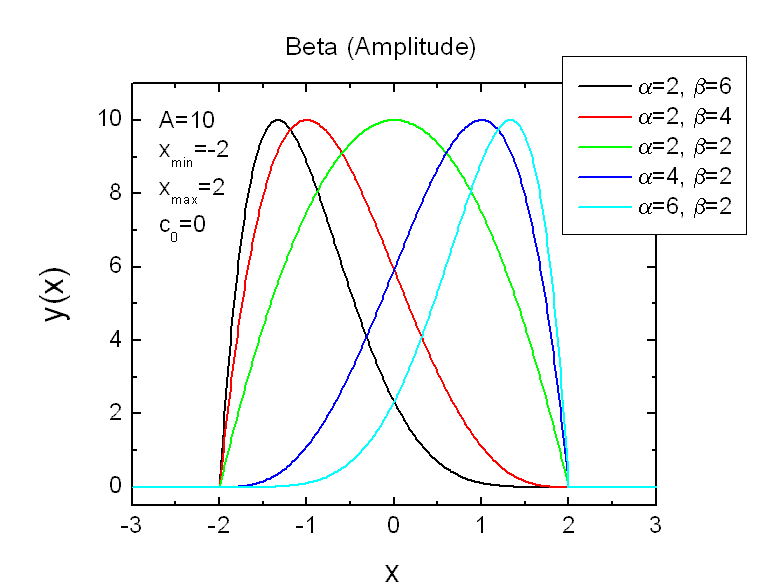
\includegraphics[width=0.768\textwidth]{BetaAmplitude.png}
\end{center}
\caption{Plot of \texttt{Beta (Amplitude)} distribution.}
\label{fig:BetaAmplitude}
\end{figure}
\vspace{5mm}

\subsection{Beta (Area)}\hspace{1pt}
\label{sec:BetaArea}

\begin{equation}
y_\mathrm{Beta (area)}\left(x;A,x_\mathrm{min},x_\mathrm{max},\alpha,\beta,c_0\right)
= A\, \frac{p_\mathrm{Beta}\left(\frac{x-x_\mathrm{min}}{x_\mathrm{max}-x_\mathrm{min}};\alpha,\beta\right)}{x_\mathrm{max}-x_\mathrm{min}}
+c_0
\end{equation}

\underline{Required parameters:}
\begin{description}
    \item[area] area $A$ of the beta distribution
    \item[xmin] continuous lower boundary parameters $x_\mathrm{min}$
    \item[xmax] continuous upper boundary parameters $x_\mathrm{max}$
    \item[alpha] first shape parameter $\alpha>0$
    \item[beta]  second shape parameter $\beta>0$
    \item[backgr] offset $c_0$
\end{description}

\underline{Note}
\begin{itemize}
  \item Both shape parameter needs to be larger than zero $(\alpha,\beta>0)$
  \item where the Beta distribution is not defined the offset value is returned: \\
  $\forall x\notin (x_\mathrm{min},x_\mathrm{max})\quad y_\mathrm{Beta (area)}(x) = c_0$
  \item Default (size) distribution: Monodisperse
\end{itemize}


%%%%%%%%%%%%%%%%%%%%%%%%%%%%%%%%%%%%%%%%%%%%%%%%%%%%%%%%%%%%%%%%%%%%%%%%%%%%%%%%%%%%%%%%
\clearpage
\section{Chi-Squared} \hspace{1pt} \\
\label{sec:ChiSquared}
\footnote{\href{http://en.wikipedia.org/wiki/Chi-square_distribution}{Description
taken partly from Wikipedia, the free encyclopedia}}In probability
theory and statistics, the chi-square distribution (also chi-squared
or $\xi^2$  distribution) is one of the most widely used theoretical
probability distributions in inferential statistics, e.g., in
statistical significance tests. It is useful because, under
reasonable assumptions, easily calculated quantities can be proven
to have distributions that approximate to the chi-square
distribution if the null hypothesis is true.

The best-known situations in which the chi-square distribution are
used are the common chi-square tests for goodness of fit of an observed
distribution to a theoretical one, and of the independence of two criteria
of classification of qualitative data. Many other statistical tests also
lead to a use of this distribution, like Friedman's analysis of variance by ranks.


A probability density function of the chi-square distribution is
\begin{equation}
    f(x;k)= \begin{cases}\displaystyle \frac{1}{2^{k/2}\Gamma(k/2)}\,x^{(k/2) - 1} e^{-x/2}&\text{for }x>0\\
                            0&\text{for }x\le 0
            \end{cases}
\end{equation}
where $\Gamma$ denotes the Gamma function, which has closed-form values at the half-integers.
The mode of the distribution is
\begin{equation}
\mathrm{mode} = k-2\, \mbox{ if }\, k\geq 2.
\end{equation}
The $\chi^2$ distribution is a special case of the gamma distribution \ref{sec:GammaDistr}
where $\theta = 2$ in the equation \ref{eq:GammaDistr}.

\subsection{Chi-Squared (Amplitude)} \hspace{1pt} \\
\label{sec:ChiSquaredAmplitude}
\begin{equation}
\chi^2(x;A,x_c,\sigma,k,c_0) =
\begin{cases}
c_0+A_0 \left(z+u\right)^{v} \exp\left(-\frac{z+u}{2}\right) & \mbox{ for } z+u \geq 0 \\
c_0 & \mbox{ otherwise}
\end{cases}
\end{equation}
with
\begin{align}
z &= \frac{x-x_x}{\sigma} \\
u &= k-2 \\
v &= \frac{k}{2}-1 \\
A_0 &= \frac{A\exp(v)}{u^v}
\end{align}
The standard statistical form has been reparameterized. The parameter $x_c$ has been added
to enable variable $x$ positioning, and $\sigma$ to enable scaling. The mode is $x_c$.
The function returns 0 for those x where it is undefined $(z+u<0)$.

\vspace{5mm}

\underline{Required parameters:}
\begin{description}
    \item[amplitude] amplitude $a$ of the Gamma peak
    \item[center] location parameter (mode) $x_c$
    \item[width] scaling parameter $\sigma>0$
    \item[shape] shape parameter $k>2$
    \item[backgr] offset $c_0$
\end{description}

\underline{Note}
\begin{itemize}
  \item The width parameter needs to be larger than zero $(\sigma>0)$.
  \item The shape parameter needs to be larger than two $(k>2)$
  \item Default (size) distribution: Monodisperse
\end{itemize}

\begin{figure}[htb]
\begin{center}
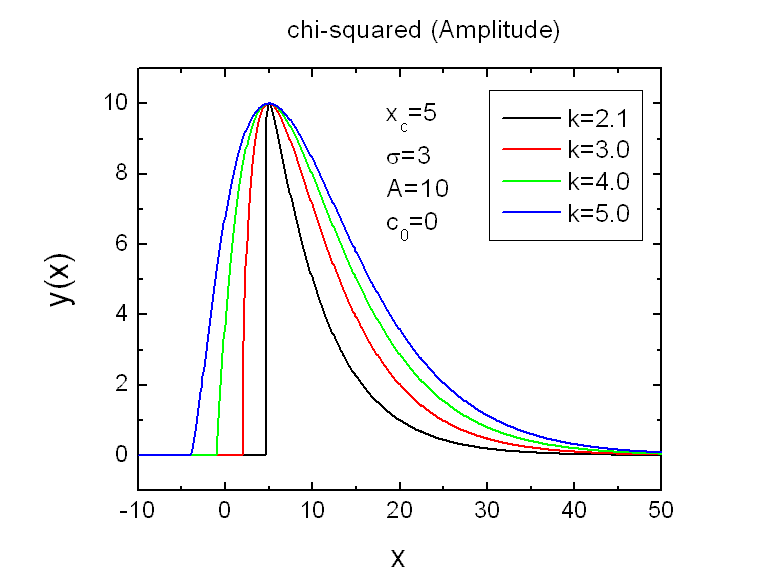
\includegraphics[width=0.768\textwidth]{ChiSquaredAmplitude.png}
\end{center}
\caption{Plot of \texttt{Chi-Squared (Amplitude)} distribution.}
\label{fig:ChiSquaredAmplitude}
\end{figure}
%%%%%%%%%%%%%%%%%%%%%%%%%%%%%%%%%%%%%%%%%%%%%%%%%%%%%%%%%%%%%%%%%%%%%%%%%%%%%%%%
%\clearpage
\subsection{Chi-Squared (Area)} ~\\
\label{sec:ChiSquaredArea}
\begin{equation}
\chi^2(x;A,x_c,\sigma,k,c_0) =
\begin{cases}
c_0+A_0 \left(z+u\right)^{v} \exp\left(-\frac{z+u}{2}\right) & \mbox{ for } z+u \geq 0 \\
c_0 & \mbox{ otherwise}
\end{cases}
\end{equation}
with
\begin{align}
z &= \frac{x-x_x}{\sigma} \\
u &= k-2 \\
v &= \frac{k}{2}-1 \\
A_0 &= \frac{A}{ 2^{\frac{k}{2}} \sigma\Gamma\left(\frac{k}{2}\right)}
\end{align}
The standard statistical form has been reparameterized. The parameter $x_c$ has been added
to enable variable $x$ positioning, and $\sigma$ to enable scaling. The mode is $x_c$.
The function returns 0 for those x where it is undefined $(z+u<0)$.

\vspace{5mm}

\underline{Required parameters:}
\begin{description}
    \item[area] area $a$ of the Gamma peak
    \item[center] location parameter (mode) $x_c$
    \item[width] scaling parameter $\sigma>0$
    \item[shape] shape parameter $k>2$
    \item[backgr] offset $c_0$
\end{description}

\underline{Note}
\begin{itemize}
  \item The width parameter needs to be larger than zero $(\sigma>0)$.
  \item The shape parameter needs to be larger than two $(k>2)$
  \item Default (size) distribution: Monodisperse
\end{itemize}
\begin{figure}[htb]
\begin{center}
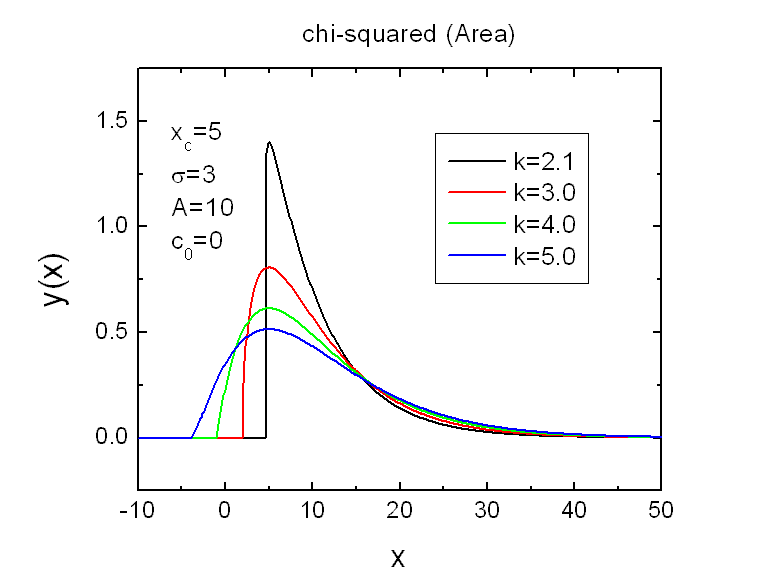
\includegraphics[width=0.768\textwidth]{ChiSquaredArea.png}
\end{center}
\caption{Plot of \texttt{Chi-Squared (Area)} distribution.}
\label{fig:ChiSquaredArea}
\end{figure}

\clearpage
\section{Erfc peak}
\label{sec:ErfcPeak}
\subsection{Erfc (Amplitude)} \hspace{1pt} \\
\label{sec:ErfcPeakAmplitude}
\begin{equation}
y(x;a,x_c,\sigma,c_0) = a \, \textrm{erfc}\left(\left(\frac{x-x_c}{\sigma}\right)^2\right)+c_0
\end{equation}
\vspace{5mm}

\underline{Required parameters:}
\begin{description}
    \item[ampl.] amplitude $a$ of the erfc peak
    \item[center] location parameter (mode) $x_c$
    \item[width] scaling parameter $\sigma>0$
    \item[backgr] offset $c_0$
\end{description}

\underline{Note}
\begin{itemize}
  \item The width parameter needs to be non-zero $(\sigma\neq 0)$.
  \item Default (size) distribution: Monodisperse
\end{itemize}
\begin{figure}[htb]
\begin{center}
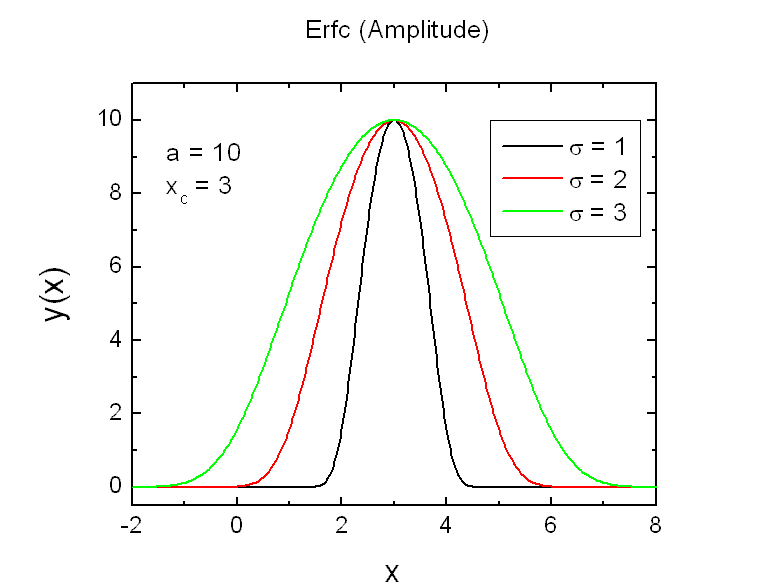
\includegraphics[width=0.768\textwidth]{ErfcAmplitude.png}
\end{center}
\caption{Plot of \texttt{Erfc (Amplitude)} distribution.}
\label{fig:ErfcAmplitude}
\end{figure}

%%%%%%%%%%%%%%%%%%%%%%%%%%%%%%%%%%%%%%%%%%%%%%%%%%%%%%%%%%%%%%%%%%%%%%%%%%%%%%%%
\clearpage
\subsection{Erfc (Area)} ~\\
\label{sec:ErfcPeakArea}
\begin{equation}
y(x;a,x_c,\sigma,c_0) = a\, \frac{\textrm{erfc}\left(\left(\frac{x-x_c}{\sigma}\right)^2\right)}{
\int_{-\infty}^{\infty}\textrm{erfc}\left(\left(\frac{x-x_c}{\sigma}\right)^2\right) \, dx}
+c_0
\end{equation}
\vspace{5mm}

\underline{Required parameters:}
\begin{description}
    \item[area] area $a$ below the erfc peak
    \item[center] location parameter (mode) $x_c$
    \item[width] scaling parameter $\sigma>0$
    \item[backgr] offset $c_0$
\end{description}

\underline{Note}
\begin{itemize}
  \item The width parameter needs to be non-zero $(\sigma\neq 0)$.
  \item Default (size) distribution: Monodisperse
\end{itemize}
\begin{figure}[htb]
\begin{center}
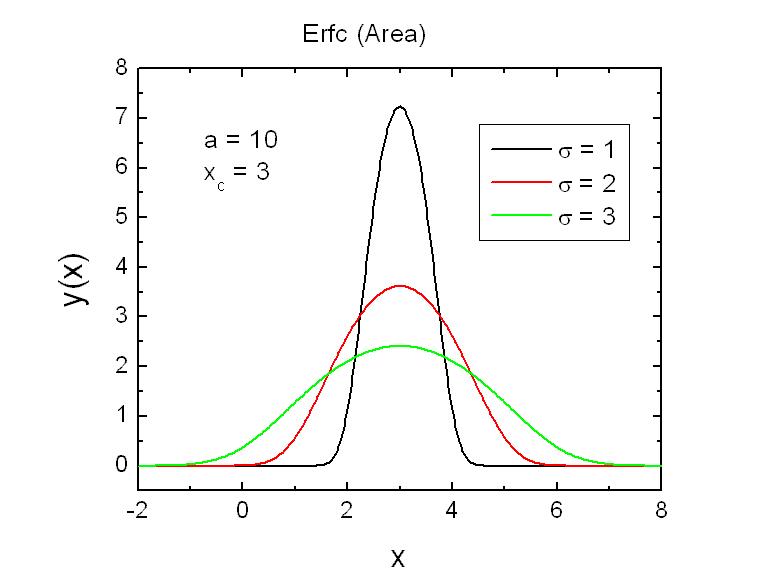
\includegraphics[width=0.768\textwidth]{ErfcArea.png}
\end{center}
\caption{Plot of \texttt{Erfc (Area)} distribution.}
\label{fig:ErfcArea}
\end{figure}

%%%%%%%%%%%%%%%%%%%%%%%%%%%%%%%%%%%%%%%%%%%%%%%%%%%%%%%%%%%%%%%%%%%%%%%%%%%%%%%%
\clearpage
\section{Error peak}
\label{sec:ErrorPeak}
\subsection{Error (Amplitude)} \hspace{1pt} \\
\label{sec:ErrorPeakAmplitude}
\begin{equation}
y(x;a,x_c,\sigma,k,c_0) = a \, \exp\left(-\frac{1}{2}\frac{\left|x-x_c\right|^{\frac{2}{k}}}{\left|\sigma\right|}\right)+c_0
\end{equation}
\vspace{5mm}

\underline{Required parameters:}
\begin{description}
    \item[ampl.] amplitude $a$ of the error distribution
    \item[center] location parameter (mode) $x_c$
    \item[width] scaling parameter $\sigma\neq 0$
    \item[shape] shape parameter $k>0$
    \item[backgr] offset $c_0$
\end{description}

\underline{Note}
\begin{itemize}
  \item The width parameter needs to be non-zero $(\sigma\neq 0)$.
  \item The shape parameter needs to be larger than zero $(k>0)$.
  \item Default (size) distribution: Monodisperse
\end{itemize}
\begin{figure}[htb]
\begin{center}
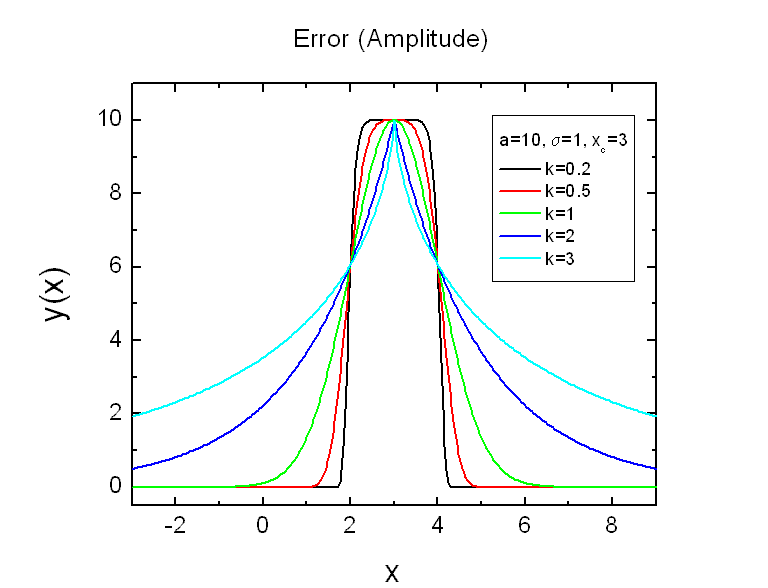
\includegraphics[width=0.768\textwidth]{ErrorAmplitude.png}
\end{center}
\caption{Plot of \texttt{Error (Amplitude)} distribution.}
\label{fig:ErrorAmplitude}
\end{figure}

%%%%%%%%%%%%%%%%%%%%%%%%%%%%%%%%%%%%%%%%%%%%%%%%%%%%%%%%%%%%%%%%%%%%%%%%%%%%%%%%
\clearpage
\subsection{Error (Area)} ~\\
\label{sec:ErrorPeakArea}
\begin{equation}
y(x;a,x_c,\sigma,k,c_0) = \frac{a}{\left|\sigma\right|^{\frac{k}{2}}2^{\frac{k}{2}+1}\Gamma\left(\frac{k}{2}+1\right)}
\, \exp\left(-\frac{1}{2}\frac{\left|x-x_c\right|^{\frac{2}{k}}}{\left|\sigma\right|}\right)+c_0
\end{equation}
\vspace{5mm}
\vspace{5mm}

\underline{Required parameters:}
\begin{description}
    \item[area] area $a$ below the error distribution
    \item[center] location parameter (mode) $x_c$
    \item[width] scaling parameter $\sigma\neq 0$
    \item[shape] shape parameter $k>0$
    \item[backgr] offset $c_0$
\end{description}

\underline{Note}
\begin{itemize}
  \item The width parameter needs to be non-zero $(\sigma\neq 0)$.
  \item The shape parameter needs to be larger than zero $(k>0)$.
  \item Default (size) distribution: Monodisperse
\end{itemize}
\begin{figure}[htb]
\begin{center}
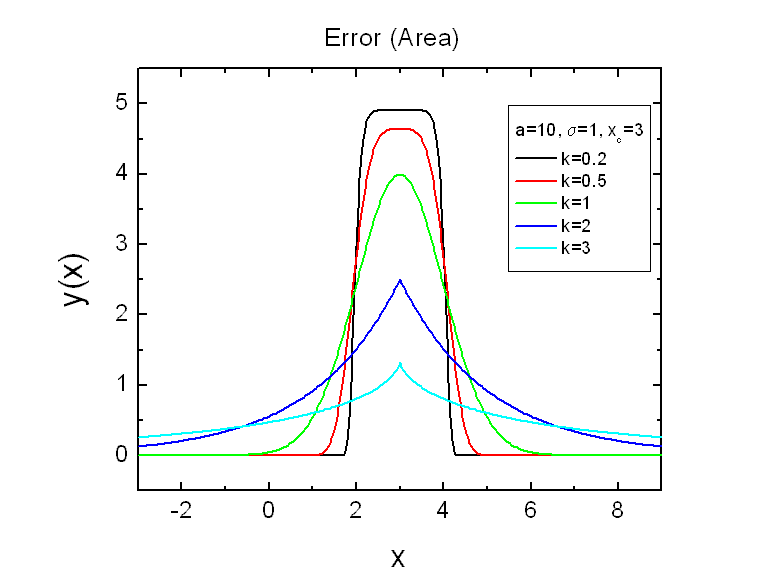
\includegraphics[width=0.768\textwidth]{ErrorArea.png}
\end{center}
\caption{Plot of \texttt{Error (Area)} distribution.}
\label{fig:ErrorArea}
\end{figure}

%%%%%%%%%%%%%%%%%%%%%%%%%%%%%%%%%%%%%%%%%%%%%%%%%%%%%%%%%%%%%%%%%%%%%%%%%%%%%%%%
\clearpage
\section{Exponentially Modified Gaussian} ~\\
\label{sec:ExponentiallyModifiedGaussian}
\subsection{Exponentially Modified Gaussian (Amplitude)} \hspace{1pt} \\
\label{sec:ExponentiallyModifiedGaussianAmplitude}
\begin{eqnarray}
y(x;a,x_c,\sigma,\gamma,c_0) & = &
\frac{a}{\mathrm{const}}
\exp\left(\frac{\sigma^2}{2\gamma^2}+\frac{x_c-x}{\gamma}\right) \nonumber \\
& & \left[\mathrm{erf}\left(\frac{x-x_c}{\sqrt{2}\sigma}-\frac{\sigma}{\sqrt{2}\gamma}\right)+\frac{\gamma}{| \gamma |}\right]
+c_0
\end{eqnarray}
$\mbox{const}$ is calculated numerically so that "$a$" represents the amplitude of the distribution.
\vspace{5mm}

\underline{Required parameters:}
\begin{description}
    \item[ampl.] amplitude $a$ of the distribution
    \item[center] location parameter $x_c$
    \item[width] scaling parameter $\sigma> 0$
    \item[distortion] distortion parameter $\gamma\neq 0$
    \item[backgr] offset $c_0$
\end{description}

\underline{Note}
\begin{itemize}
  \item The width parameter needs to be non-zero $(\sigma\neq 0)$.
  \item The distortion parameter needs to be non-zero $(\gamma \neq 0)$.
  \item Default (size) distribution: Monodisperse
\end{itemize}
\begin{figure}[htb]
\begin{center}
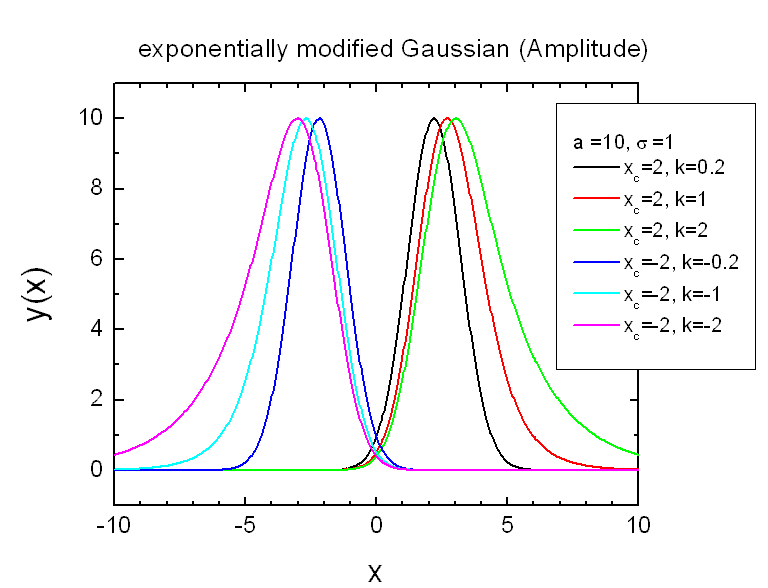
\includegraphics[width=0.768\textwidth]{EMGAmplitude.png}
\end{center}
\caption{Plot of \texttt{Exponentially Modified Gaussian (Amplitude)} distribution.}
\label{fig:EMGAmplitude}
\end{figure}

%%%%%%%%%%%%%%%%%%%%%%%%%%%%%%%%%%%%%%%%%%%%%%%%%%%%%%%%%%%%%%%%%%%%%%%%%%%%%%%%
\clearpage
\subsection{Exponentially Modified Gaussian (Area)} ~\\
\label{sec:ExponentiallyModifiedGaussianArea}
\begin{eqnarray}
y(x;a,x_c,\sigma,\gamma,c_0) & = &
\frac{a}{2\gamma}
\exp\left(\frac{\sigma^2}{2\gamma^2}+\frac{x_c-x}{\gamma}\right) \nonumber \\
& & \left[\mathrm{erf}\left(\frac{x-x_c}{\sqrt{2}\sigma}-\frac{\sigma}{\sqrt{2}\gamma}\right)+\frac{\gamma}{| \gamma |}\right]
+c_0
\end{eqnarray}

\vspace{5mm}

\underline{Required parameters:}
\begin{description}
    \item[area] area $a$ below the distribution
    \item[center] location parameter $x_c$
    \item[width] scaling parameter $\sigma> 0$
    \item[distortion] distortion parameter $\gamma\neq 0$
    \item[backgr] offset $c_0$
\end{description}

\underline{Note}
\begin{itemize}
  \item The width parameter needs to be non-zero $(\sigma> 0)$.
  \item The distortion parameter needs to be non-zero $(\gamma \neq 0)$.
  \item Default (size) distribution: Monodisperse
\end{itemize}
\begin{figure}[htb]
\begin{center}
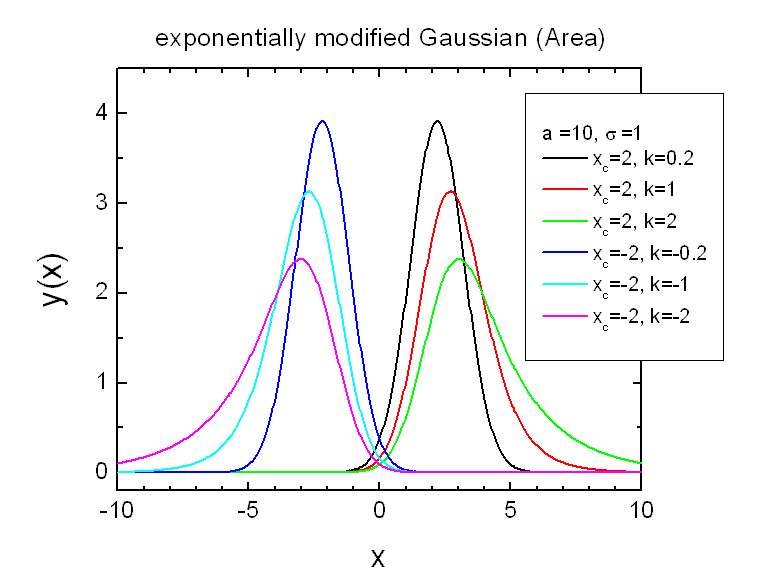
\includegraphics[width=0.768\textwidth]{EMGArea.png}
\end{center}
\caption{Plot of \texttt{Exponentially Modified Gaussian (Area)} distribution.}
\label{fig:EMGArea}
\end{figure}

%%%%%%%%%%%%%%%%%%%%%%%%%%%%%%%%%%%%%%%%%%%%%%%%%%%%%%%%%%%%%%%%%%%%%%%%%%%%%%%%
\clearpage

\section{Extreme Value} ~\\
\label{sec:ExtremeValue}
\subsection{Extreme Value (Amplitude)} \hspace{1pt} \\
\label{sec:ExtremeValueAmplitude}
\begin{equation}
y(x;a,x_c,\sigma,c_0) = a \,
\exp\left[-\exp\left(-\frac{x-x_c}{|\sigma|}\right)-\frac{x-x_c}{|\sigma|}+1\right]
+c_0
\end{equation}
\vspace{5mm}

\underline{Required parameters:}
\begin{description}
    \item[ampl.] amplitude $a$ of the peak
    \item[center] location parameter (mode) $x_c$
    \item[width] scaling parameter $\sigma\neq 0$
    \item[backgr] offset $c_0$
\end{description}

\underline{Note}
\begin{itemize}
  \item The width parameter needs to be non-zero $(\sigma\neq 0)$.
  \item Default (size) distribution: Monodisperse
\end{itemize}
\begin{figure}[htb]
\begin{center}
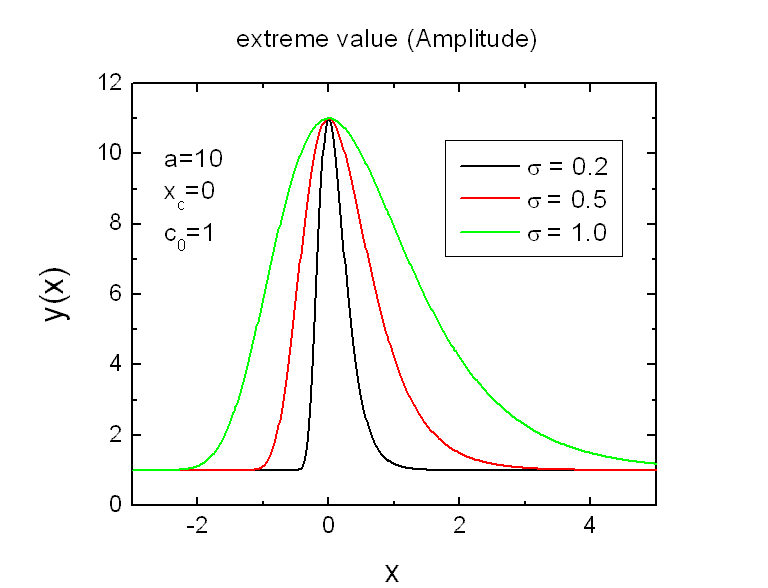
\includegraphics[width=0.768\textwidth]{ExtremeValueAmplitude.png}
\end{center}
\caption{Plot of \texttt{extreme value (Amplitude)} distribution.}
\label{fig:ExtremeValueAmplitude}
\end{figure}

%%%%%%%%%%%%%%%%%%%%%%%%%%%%%%%%%%%%%%%%%%%%%%%%%%%%%%%%%%%%%%%%%%%%%%%%%%%%%%%%
\clearpage
\subsection{Extreme Value (Area)} ~\\
\label{sec:ExtremeValueArea}
\begin{equation}
y(x;a,x_c,\sigma,c_0) = \frac{a}{|\sigma|} \,
\exp\left[-\exp\left(-\frac{x-x_c}{|\sigma|}\right)-\frac{x-x_c}{|\sigma|}\right]
+c_0
\end{equation}
\vspace{5mm}

\underline{Required parameters:}
\begin{description}
    \item[area] area $a$ below the peak
    \item[center] location parameter (mode) $x_c$
    \item[width] scaling parameter $\sigma \neq 0$
    \item[backgr] offset $c_0$
\end{description}

\underline{Note}
\begin{itemize}
  \item The width parameter needs to be non-zero $(\sigma\neq 0)$.
  \item Default (size) distribution: Monodisperse
\end{itemize}
\begin{figure}[htb]
\begin{center}
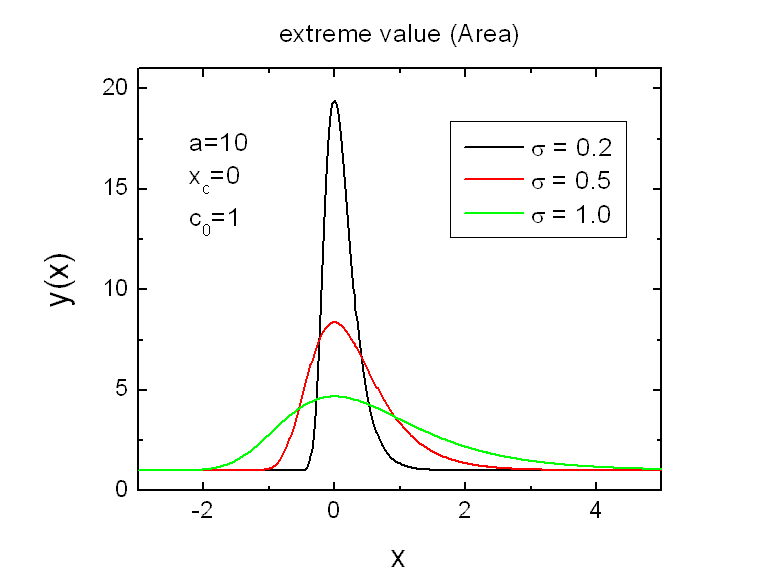
\includegraphics[width=0.768\textwidth]{ExtremeValueArea.png}
\end{center}
\caption{Plot of \texttt{extreme value (Area)} distribution.}
\label{fig:ExtremeValueArea}
\end{figure}

%%%%%%%%%%%%%%%%%%%%%%%%%%%%%%%%%%%%%%%%%%%%%%%%%%%%%%%%%%%%%%%%%%%%%%%%%%%%%%%%
\clearpage

\section{F-Variance} ~\\
\label{sec:FVariance}

In probability theory and statistics, the
F-distribution is a continuous probability distribution. It is also
known as Snedecor's F distribution or the Fisher-Snedecor
distribution. The probability density is given by
\begin{equation}
p_\mathrm{F-var}(x,\nu_1,\nu_2) =
\frac{\DS \sqrt{\frac{\left(\nu_1 x\right)^{\nu_1} \nu_2^{\nu_2}}{\left(\nu_1 x+\nu_2\right)^{\nu_1+\nu_2}}}}{x\,\mathrm{B}\left(\frac{\nu_1}{2},\frac{\nu_2}{2}\right)}
%   \frac{ \Gamma\left(\frac{\nu_1 + \nu_2}{2}\right)
%        }{ \Gamma\left(\frac{\nu_1}{2}\right) \Gamma\left(\frac{\nu_2}{2}\right) }
%   \nu_1^\frac{\nu_1}{2} \nu_2^\frac{\nu_2}{2}
%   x^{\frac{\nu_1}{2} - 1} (\nu_2 + \nu_1 x)^{-\frac{\nu_1}{2}-\frac{\nu_2}{2}}
\end{equation}
for real $x\geq 0$, where $\nu>1$ and $\nu_2$ are positive,
and $\mathrm{B}()$  is the beta function.
For $\nu_1>2$ the mode of the distribution is defined by
\begin{equation}
\mathrm{mode}_F(\nu_1,\nu_2)=\frac{\nu_1-2}{\nu_1}\frac{\nu_2}{\nu_2+2}
\end{equation}
\vspace{5mm}

\subsection{F-Variance (Amplitude)} ~\\
\label{sec:FVarianceAmplitude}
The amplitude version represents a re-parametrization of the standard statistical form.
\begin{align}
y(x;a,x_c,\sigma,\nu_1,\nu_2)
&=
\begin{cases}
c_0+a\,\frac{p_\mathrm{F-var}(z,\nu_1,\nu_2)}{p_\mathrm{F-var}(\mathrm{mode}_F(\nu_1,\nu_2),\nu_1,\nu_2)}  & \mbox{ for } z>0\\
c_0 & \mbox{ otherwise}
\end{cases} \nonumber\\
&=
\begin{cases}
c_0+a\,\frac{z^{\frac{\nu_1}{2}-1}\left(1+\frac{\nu_1-2}{\nu_2+2}\right)^{\frac{\nu_1+\nu2}{2}}}{\left(1+\frac{\nu1}{\nu2}z\right)^{\frac{\nu_1+\nu_2}{2}}\left(\frac{\nu_2}{\nu_1}\frac{\nu_1-2}{\nu_2+2}\right)^{\frac{\nu_1}{2}-1}}   & \mbox{ for } z>0\\
c_0 & \mbox{ otherwise}
\end{cases}
\end{align}
with
\begin{equation}
z = \frac{x-x_c}{\sigma}+\frac{\nu_1-2}{\nu_1}\frac{\nu_2}{\nu_2+2}
\end{equation}
The location parameter $x_c$ has been added to enable variable $x$ positioning, and $\sigma$
to enable scaling. The mode of the distribution function is $x_c$ due to the additional term
$\frac{\nu_1-2}{\nu_1}\frac{\nu_2}{\nu_2+2}$ in the definition of $z$. The distribution
function returns the offset $c_0$ for values $z\leq 0$.

\vspace{5mm}

\underline{Required parameters:}
\begin{description}
    \item[ampl.] amplitude $a$ of the F-distribution
    \item[center] location parameter (mode) $x_c$
    \item[width] scaling parameter $\sigma>0$
    \item[shape1] shape parameter $\nu_1>2$
    \item[shape2] shape parameter $\nu_2>2$
    \item[backgr] offset $c_0$
\end{description}

\underline{Note}
\begin{itemize}
  \item The scale parameter needs to be larger than zero $\sigma>0$
  \item The first shape parameter needs to be larger than zero $\nu_1>2$
  \item The second shape parameter needs to be larger than zero $\nu_2>2$
  \item Default (Size) distribution: Monodisperse
\end{itemize}

\begin{figure}[htb]
\begin{center}
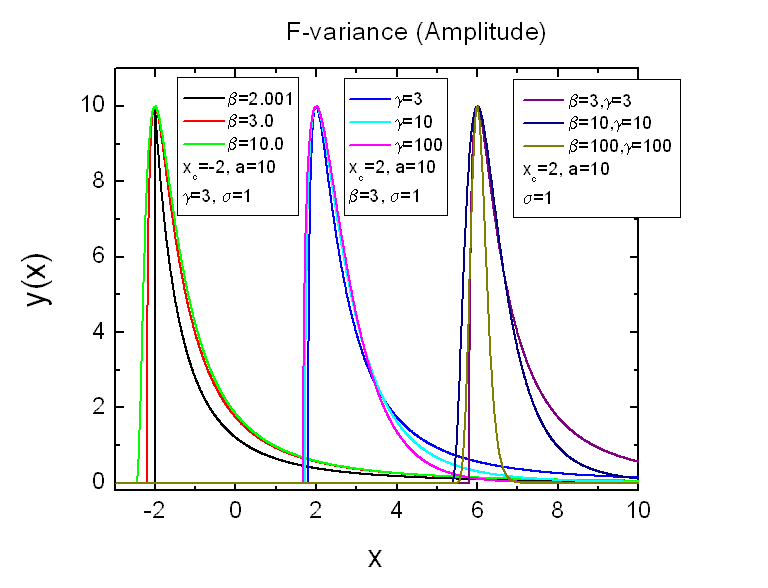
\includegraphics[width=0.768\textwidth]{FvarianceAmplitude.png}
\end{center}
\caption{Plot of \texttt{F-variance (Amplitude)} distribution.}
\label{fig:FvarianceAmplitude}
\end{figure}

\vspace{5mm}
\subsection{F-Variance (Area)} ~\\
\label{sec:FVarianceArea}
The area version represents a re-parametrization of the standard statistical form.
\begin{align}
y(x;a,x_c,\sigma,\nu_1,\nu_2)
&=
\begin{cases}
c_0+\frac{a}{\sigma}\,p_\mathrm{F-var}(z,\nu_1,\nu_2) & \mbox{ for } z>0\\
c_0 & \mbox{ otherwise}
\end{cases}
\end{align}
with
\begin{equation}
z = \frac{x-x_c}{\sigma}+\frac{\nu_1-2}{\nu_1}\frac{\nu_2}{\nu_2+2}
\end{equation}
The location parameter $x_c$ has been added to enable variable $x$ positioning, and $\sigma$
to enable scaling. The mode of the distribution function is $x_c$ due to the additional term
$\frac{\nu_1-2}{\nu_1}\frac{\nu_2}{\nu_2+2}$ in the definition of $z$. The distribution
function returns the offset $c_0$ for values $z\leq 0$.

\vspace{5mm}
\underline{Required parameters:}
\begin{description}
    \item[area] area $a$ of the F-distribution
    \item[center] location parameter (mode) $x_c$
    \item[width] scaling parameter $\sigma>0$
    \item[shape1] shape parameter $\nu_1>2$
    \item[shape2] shape parameter $\nu_2>2$
    \item[backgr] offset $c_0$
\end{description}

\underline{Note}
\begin{itemize}
  \item The scale parameter needs to be larger than zero $\sigma>0$
  \item The first shape parameter needs to be larger than zero $\nu_1>2$
  \item The second shape parameter needs to be larger than zero $\nu_2>2$
  \item Default (Size) distribution: Monodisperse
\end{itemize}

\begin{figure}[htb]
\begin{center}
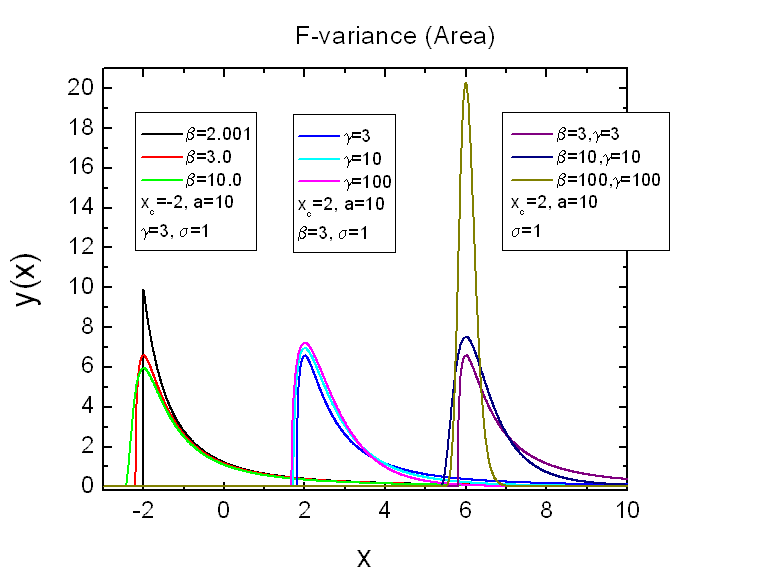
\includegraphics[width=0.768\textwidth]{FvarianceArea.png}
\end{center}
\caption{Plot of \texttt{F-variance (Area)} distribution.}
\label{fig:FVarianceArea}
\end{figure}

%%%%%%%%%%%%%%%%%%%%%%%%%%%%%%%%%%%%%%%%%%%%%%%%%%%%%%%%%%%%%%%%%%%%%%%%%%%%%%%%
\clearpage
\section{Gamma}
\label{sec:GammaDistr}
The gamma distribution models sums of exponentially distributed random variables.

The gamma distribution family is based on two parameters. The
chi-square and exponential distributions, which are children of the
gamma distribution, are one-parameter distributions that fix one of
the two gamma parameters. The standard form is given by
\begin{equation}
\label{eq:GammaDistr}
p(x;k,\theta) = x^{k-1} \frac{e^{-x/\theta}}{\theta^k
\, \Gamma(k)} \ \mathrm{ for }\ x > 0\,\, \mathrm{ and }\,\, k,
\theta > 0.
\end{equation}
When $k$ is large, the gamma distribution closely approximates a
normal distribution with the advantage that the gamma distribution
has density only for positive real numbers.
In probability theory and statistics, the gamma distribution is a
two-parameter family of continuous probability distributions.
It has a scale parameter $\theta$ and a shape parameter $k$. If $k$
is an integer then the distribution represents the sum of $k$ independent
exponentially distributed random variables, each of which has a mean of
$\theta$ (which is equivalent to a rate parameter of $\theta^{-1}$).


Alternatively, the gamma distribution can be parameterized
in terms of a shape parameter $\alpha = k$ and an inverse scale
parameter $\beta = 1/\theta$, called a rate parameter:
\begin{equation}
p(x;\alpha,\beta) = x^{\alpha-1} \frac{\beta^{\alpha} \,
e^{-\beta\,x} }{\Gamma(\alpha)} \ \mathrm{for}\ x > 0 \,\!.
\end{equation}

\vspace{5mm}

\subsection{Gamma (Amplitude)} ~\\
\label{sec:GammaDistrAmplitude}
  The parameter $x_c$ has been added to enable variable $x$ positioning,
  whereas the $+\theta(k-1)$ adjusts $x_c$ so that it represents the mode.
  $c_0$ is the offset value.
  The function returns the offset $c_0$ for those $x$ where it is undefined

  \begin{equation}
   y(x) = \Bigg\{
   \begin{array}{ll}
       c_0 + a \exp(-z) \left(\frac{z+k-1}{k-1}\right)^{k-1} & \mbox{for } (z+k-1) > 0 \\
       c_0 &  \mbox{otherwise}
   \end{array}
  \end{equation}
  with $ z=\frac{x-x_c}{\theta} $

~\\

\underline{Required parameters:}
\begin{description}
    \item[ampl.] amplitude $a$ of the Gamma peak
    \item[center] location parameter (mode) $x_c$
    \item[width] scaling parameter $\theta>0$
    \item[backgr] offset $c_0$
\end{description}

\underline{Note}
\begin{itemize}
  \item The shape parameter needs to be larger than one $k>1$.
  \item The scale parameter needs to be larger than zero $\theta>0$
  \item Default (Size) distribution: Monodisperse
\end{itemize}

\begin{figure}[htb]
\begin{center}
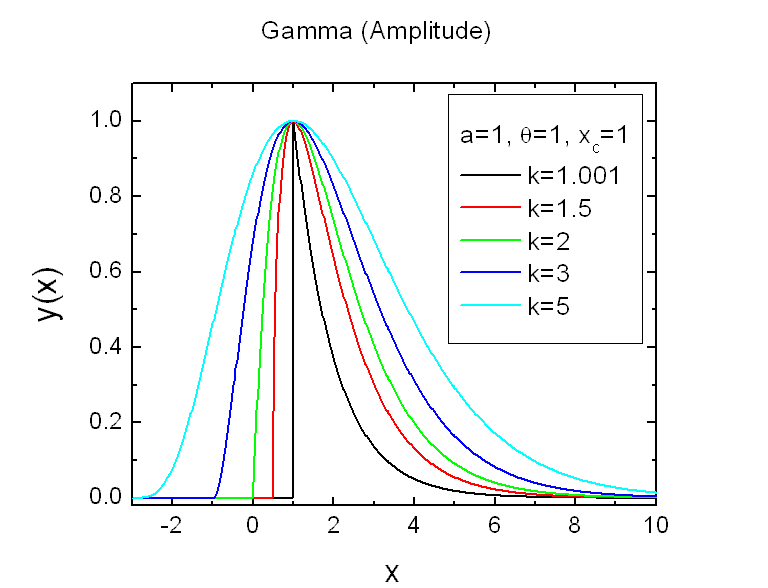
\includegraphics[width=0.768\textwidth]{GammaAmplitude.png}
\end{center}
\caption{Plot of \texttt{Gamma (Amplitude)} distribution.}
\label{fig:GammaAmplitude}
\end{figure}

\vspace{5mm}

\subsection{Gamma (Area)} ~\\
\label{sec:GammaDistrArea}

  The parameter $x_c$ has been added to enable variable $x$ positioning,
  whereas the $+\theta(k-1)$ adjusts $x_c$ so that it represents the mode.
  $c_0$ is the offset value.
  The function returns the offset $c_0$ for those $x$ where it is undefined

\begin{equation}
       y(x) = \Bigg\{
       \begin{array}{ll}
           c_0 + \frac{a}{\theta\Gamma(k)} \exp(-z) z^{k-1} & \mbox{for } z > 0 \\
           c_0 &  \mbox{otherwise}
       \end{array}
\end{equation}
with $z=\frac{x-x_c}{\theta} +k-1$

~\\

\underline{Required parameters:}
\begin{description}
    \item[area] area $a$ of the Gamma peak
    \item[center] location parameter (mode) $x_c$
    \item[width] scaling parameter $\theta>0$
    \item[backgr] offset $c_0$
\end{description}

\underline{Note}
\begin{itemize}
  \item The shape parameter needs to be larger than one $k>1$.
  \item The scale parameter needs to be larger than zero $\theta>0$
  \item Default (Size) distribution: Monodisperse
\end{itemize}


\begin{figure}[htb]
\begin{center}
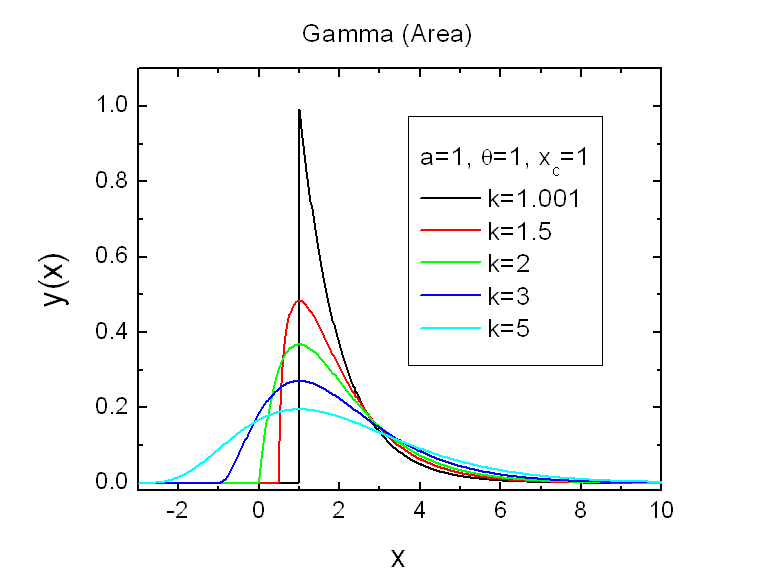
\includegraphics[width=0.768\textwidth]{GammaArea.png}
\end{center}
\caption{Plot of \texttt{Gamma (Area)} distribution.}
\label{fig:GammaArea}
\end{figure}


%%%%%%%%%%%%%%%%%%%%%%%%%%%%%%%%%%%%%%%%%%%%%%%%%%%%%%%%%%%%%%%%%%%%%%%%%%%%%%%%
\clearpage

\section{Gaussian or Normal distribution} ~\\
\label{sec:GaussianNormal}
\subsection{Gaussian (Amplitude)} \hspace{1pt} \\
\label{sec:GaussianNormalAmplitude}
\begin{equation}
y(x;a,x_c,\sigma,c_0) = a \,
\exp\left[-\frac{1}{2}\left(\frac{x-x_c}{|\sigma|}\right)^2\right]
+c_0
\end{equation}
\vspace{5mm}

\underline{Required parameters:}
\begin{description}
    \item[ampl.] amplitude $a$ of the peak
    \item[center] location parameter (mode) $x_c$
    \item[width] scaling parameter $\sigma\neq 0$
    \item[backgr] offset $c_0$
\end{description}

\underline{Note}
\begin{itemize}
  \item The width parameter needs to be non-zero $(\sigma\neq 0)$.
  \item Default (size) distribution: Monodisperse
\end{itemize}
\begin{figure}[htb]
\begin{center}
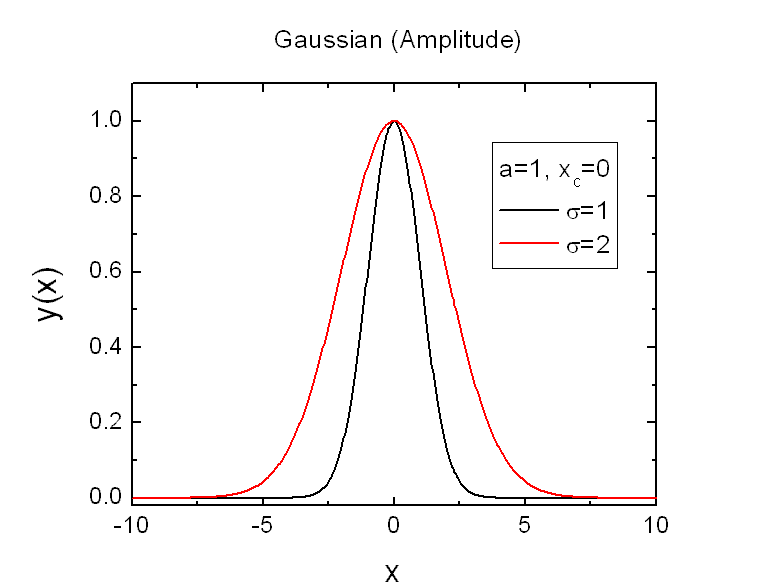
\includegraphics[width=0.768\textwidth]{GaussianAmplitude.png}
\end{center}
\caption{Plot of \texttt{Gaussian (Amplitude)} distribution.}
\label{fig:GaussianAmplitude}
\end{figure}

%%%%%%%%%%%%%%%%%%%%%%%%%%%%%%%%%%%%%%%%%%%%%%%%%%%%%%%%%%%%%%%%%%%%%%%%%%%%%%%%
\clearpage
\subsection{Gaussian (Area)} ~\\
\label{sec:GaussianNormalArea}
\begin{equation}
y(x;a,x_c,\sigma,c_0) = \frac{a}{|\sigma|\sqrt{2\pi}} \,
\exp\left[-\frac{1}{2}\left(\frac{x-x_c}{|\sigma|}\right)^2\right]
+c_0
\end{equation}
\vspace{5mm}

\underline{Required parameters:}
\begin{description}
    \item[area] area $a$ below the peak
    \item[center] location parameter (mode) $x_c$
    \item[width] scaling parameter $\sigma \neq 0$
    \item[backgr] offset $c_0$
\end{description}

\underline{Note}
\begin{itemize}
  \item The width parameter needs to be non-zero $(\sigma\neq 0)$.
  \item Default (size) distribution: Monodisperse
\end{itemize}
\begin{figure}[htb]
\begin{center}
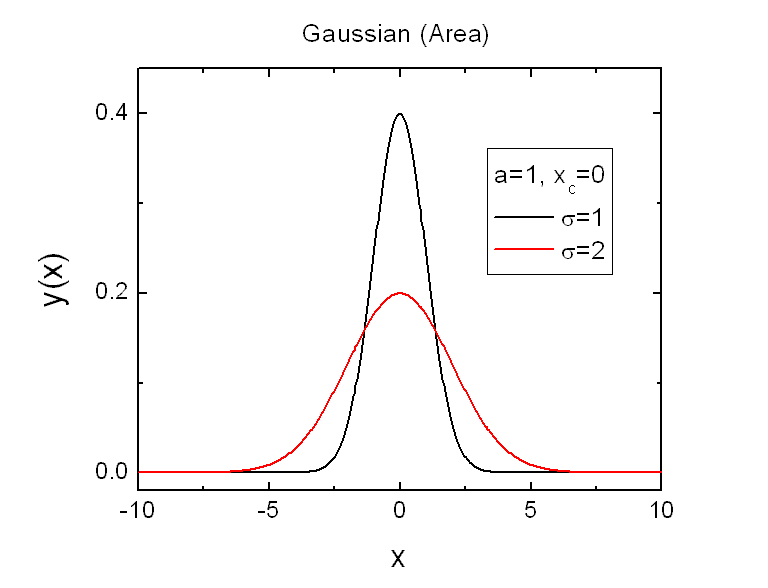
\includegraphics[width=0.768\textwidth]{GaussianArea.png}
\end{center}
\caption{Plot of \texttt{Gaussian (Area)} distribution.}
\label{fig:GaussianArea}
\end{figure}


%%%%%%%%%%%%%%%%%%%%%%%%%%%%%%%%%%%%%%%%%%%%%%%%%%%%%%%%%%%%%%%%%%%%%%%%%%%%%%%%
\clearpage
\section{Gaussian-Lorentzian cross product} ~\\
\label{sec:GaussianLorentzianCrossProduct}
This distribution function is a Voigt approximation. It combines a Gaussian and Lorentzian
in a multiplicative form. The shape parameter $\nu$ varies from 0 to 1. The pure
Lorentzian occurs with $\nu=1$ and the pure Gaussian with $\nu=0$ but the transition from
Lorentzian to Gaussian shape in not a linear function of $\nu$

\vspace{5mm} \clearpage

\subsection{Gaussian-Lorentzian cross product (Amplitude)} ~\\
\label{sec:GaussianLorentzianCrossProductAmplitude}
\begin{equation}
y(x,a,x_c,\sigma,\nu,c_0) = a\,
\frac{\exp\left(-\frac{1-\nu}{2}\left(\frac{x-x_c}{|\sigma|}\right)^2\right)}{1+\nu\left(\frac{x-x_c}{|\sigma|}\right)^2}+c_0
\end{equation}
\vspace{5mm}

\underline{Required parameters:}
\begin{description}
    \item[amplitude] amplitude $a$ of the peak
    \item[center] location parameter (mode) $x_c$
    \item[shape] shape parameter $\nu\in [0,1]$
    \item[width] scaling parameter $\sigma \neq 0$
    \item[backgr] offset $c_0$
\end{description}

\underline{Note}
\begin{itemize}
  \item The width parameter needs to be non-zero $(\sigma\neq 0)$.
  \item The shape parameter need to be between 0 and 1 ($\nu\in [0,1]$)
  \item Default (size) distribution: Monodisperse
\end{itemize}
\begin{figure}[htb]
\begin{center}
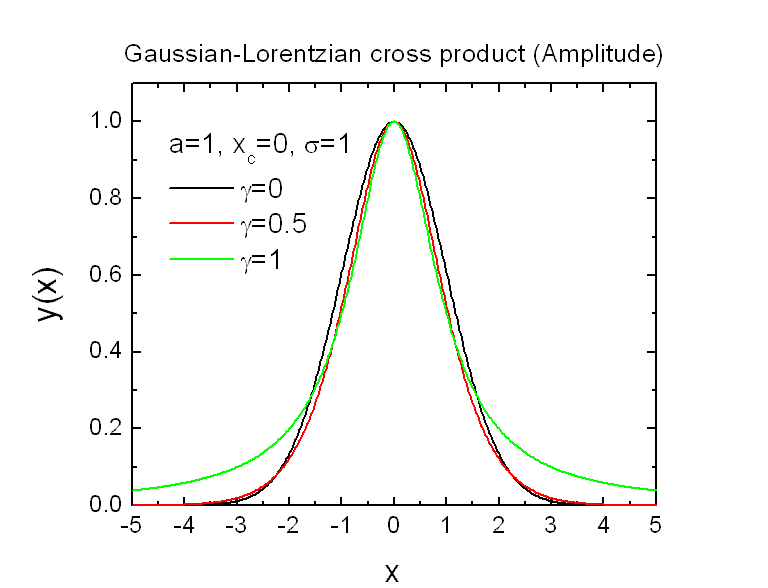
\includegraphics[width=0.768\textwidth]{GaussianLorentzianCrossProductAmplitude.png}
\end{center}
\caption{Plot of \texttt{Gaussian-Lorentzian cross product} \texttt{(Amplitude)} distribution.}
\label{fig:GaussianLorentzianCrossProductAmplitude}
\end{figure}

\clearpage

\subsection{Gaussian-Lorentzian cross product (Area)} ~\\
\label{sec:GaussianLorentzianCrossProductArea}
\begin{equation}
y(x,a,x_c,\sigma,\nu,c_0) = a\,
\frac{\sqrt{\nu}}{|\sigma|\pi}\frac{\exp\left(-\frac{1-\nu}{2\nu}\right)}{\mbox{erfc}\left(\sqrt{\frac{1-\nu}{2\nu}}\right)}
\frac{\exp\left(-\frac{1-\nu}{2}\left(\frac{x-x_c}{|\sigma|}\right)^2\right)}{1+\nu\left(\frac{x-x_c}{|\sigma|}\right)^2}
+c_0
\end{equation}

\vspace{5mm}

\underline{Required parameters:}
\begin{description}
    \item[area] area $a$ below the peak
    \item[center] location parameter (mode) $x_c$
    \item[shape] shape parameter $\nu\in [0,1]$
    \item[width] scaling parameter $\sigma \neq 0$
    \item[backgr] offset $c_0$
\end{description}

\underline{Note}
\begin{itemize}
  \item The width parameter needs to be non-zero $(\sigma\neq 0)$.
  \item The shape parameter need to be between 0 and 1 ($\nu\in [0,1]$)
  \item Default (size) distribution: Monodisperse
\end{itemize}
\begin{figure}[htb]
\begin{center}
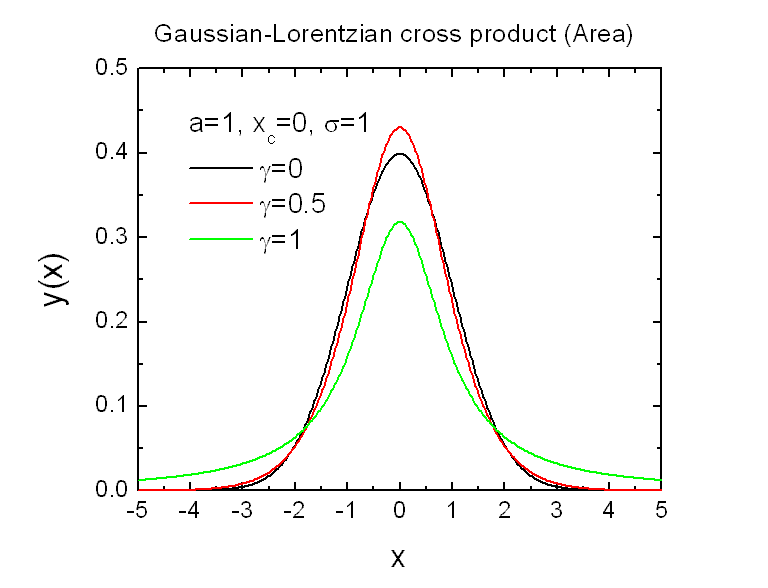
\includegraphics[width=0.768\textwidth]{GaussianLorentzianCrossProductArea.png}
\end{center}
\caption{Plot of \texttt{Gaussian-Lorentzian cross product (Area)} distribution.}
\label{fig:GaussianLorentzianCrossProductArea}
\end{figure}
%%%%%%%%%%%%%%%%%%%%%%%%%%%%%%%%%%%%%%%%%%%%%%%%%%%%%%%%%%%%%%%%%%%%%%%%%%%%%%%%
\clearpage

\section{Gaussian-Lorentzian sum} ~\\
\label{sec:GaussianLorentzianSum}
This distribution function is another Voigt approximation, which is simply a sum of
Lorentzian and Gaussian with equal FWHM. The shape parameter $\nu$ varies from 0 to 1. The pure
Lorentzian occurs with $\nu=1$ and the pure Gaussian with $\nu=0$. The width parameter $\sigma$
directly computes the full-width at half-maximum (FWHM).

\vspace{5mm} \clearpage

\subsection{Gaussian-Lorentzian sum (Amplitude)} ~\\
\label{sec:GaussianLorentzianSumAmplitude}
\begin{multline}
y(x,a,x_c,\sigma,\nu,c_0) = \\
a\,\frac{\frac{\nu}{|\sigma|}\sqrt{\frac{\ln 2}{\pi}}\exp\left(-4\ln
2\left(\frac{x-x_c}{|\sigma|}\right)^2\right)+\frac{1-\nu}{\pi|\sigma|\left[1+4\left(\frac{x-x_c}{|\sigma|}\right)^2\right]}}{\frac{\nu}{|\sigma|}\sqrt{\frac{\ln
2}{\pi}}+\frac{1-\nu}{\pi|\sigma|}} + c_0
\end{multline}

\vspace{5mm}

\underline{Required parameters:}
\begin{description}
    \item[amplitude] amplitude $a$ of the peak
    \item[center] location parameter (mode) $x_c$
    \item[shape] shape parameter $\nu\in [0,1]$
    \item[width] scaling parameter $\sigma \neq 0$
    \item[backgr] offset $c_0$
\end{description}

\underline{Note}
\begin{itemize}
  \item The width parameter needs to be non-zero $(\sigma\neq 0)$.
  \item The shape parameter need to be between 0 and 1 ($\nu\in [0,1]$)
  \item Default (size) distribution: Monodisperse
\end{itemize}
\begin{figure}[htb]
\begin{center}
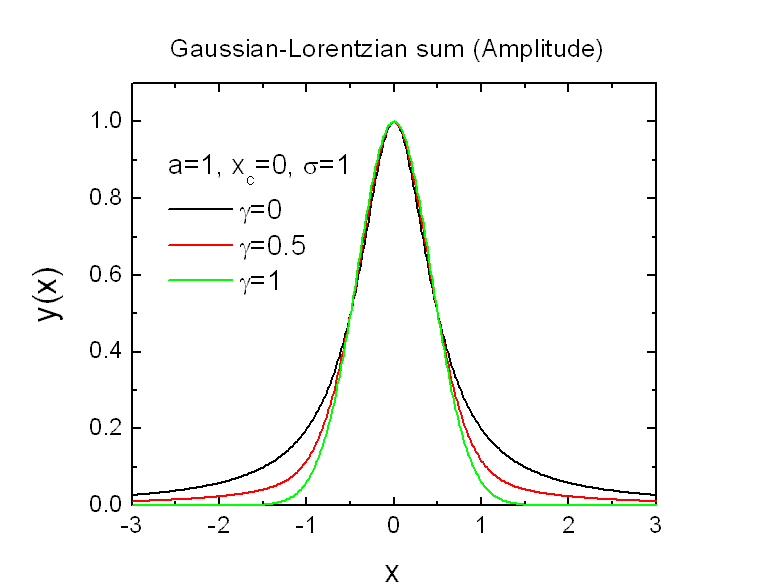
\includegraphics[width=0.768\textwidth]{GaussianLorentzianSumAmplitude.png}
\end{center}
\caption{Plot of \texttt{Gaussian-Lorentzian sum} \texttt{(Amplitude)} distribution.}
\label{fig:GaussianLorentzianSumAmplitude}
\end{figure}

\clearpage

\subsection{Gaussian-Lorentzian sum (Area)} ~\\
\label{sec:GaussianLorentzianSumArea}
\begin{multline}
y(x,a,x_c,\sigma,\nu,c_0) = \\
2a\,\left[\frac{\nu}{|\sigma|}\sqrt{\frac{\ln 2}{\pi}}\exp\left({
-4\ln
2\left(\frac{x-x_c}{|\sigma|}\right)^2}\right)+\frac{1-\nu}{\pi|\sigma|\left[1+4\left(\frac{x-x_c}{|\sigma|}\right)^2\right]}\right]+c_0
\end{multline}
\vspace{5mm}

\underline{Required parameters:}
\begin{description}
    \item[area] area $a$ below the peak
    \item[center] location parameter (mode) $x_c$
    \item[shape] shape parameter $\nu\in [0,1]$
    \item[width] scaling parameter $\sigma \neq 0$
    \item[backgr] offset $c_0$
\end{description}

\underline{Note}
\begin{itemize}
  \item The width parameter needs to be non-zero $(\sigma\neq 0)$.
  \item The shape parameter need to be between 0 and 1 ($\nu\in [0,1]$)
  \item Default (size) distribution: Monodisperse
\end{itemize}
\begin{figure}[htb]
\begin{center}
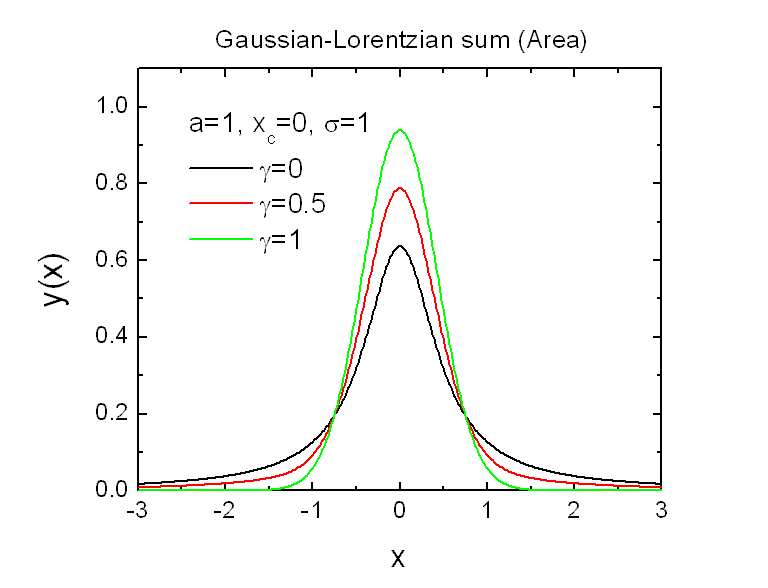
\includegraphics[width=0.768\textwidth]{GaussianLorentzianSumArea.png}
\end{center}
\caption{Plot of \texttt{Gaussian-Lorentzian sum (Area)} distribution.}
\label{fig:GaussianLorentzianSumArea}
\end{figure}

%%%%%%%%%%%%%%%%%%%%%%%%%%%%%%%%%%%%%%%%%%%%%%%%%%%%%%%%%%%%%%%%%%%%%%%%%%%%%%%%
\clearpage
\section{generalized Gaussian 1} ~\\
\label{sec:generalizedGaussian1}

The generalized Gaussian distribution is one of two families of
continuous probability distributions, which has an additional shape
parameter to the normal distribution. Known also as the exponential
power distribution, or the generalized error distribution, this is a
parametric family of symmetric distributions. It includes all normal
and Laplace distributions, and as limiting cases it includes all
continuous uniform distributions on bounded intervals of the real
line.

This family includes the normal distribution when $\beta=2$ (with
mean $\mu$ and variance $\frac{\alpha^2}{2}$) and it includes the
Laplace distribution when $\beta=1$. As $\beta\rightarrow\infty$,
the density converges pointwise to a uniform density on $
(\mu-\alpha,\mu+\alpha)$.

\clearpage
\subsection{generalized Gaussian 1 (Amplitude)} ~\\
\label{sec:generalizedGaussian1Amplitude}

\begin{align}
y(x,a,\mu,\alpha,\beta) = a e^{-\abs{\frac{x-\mu}{\alpha}}^\beta}
\end{align}

\underline{Required parameters:}
\begin{description}
    \item[amplitude] amplitude $a$ of the peak
    \item[center] location parameter (mode) $\mu$
    \item[width] scaling parameter $\alpha \neq 0$
    \item[shape] shape parameter $\beta$
    \item[backgr] offset $c_0$
\end{description}

\underline{Note}
\begin{itemize}
  \item The width parameter needs to be non-zero $(\alpha\neq 0)$.
  \item The area parameter needs to be positive $(\beta> 0)$.
  \item Default (size) distribution: Monodisperse
\end{itemize}

\begin{figure}[htb]
\begin{center}
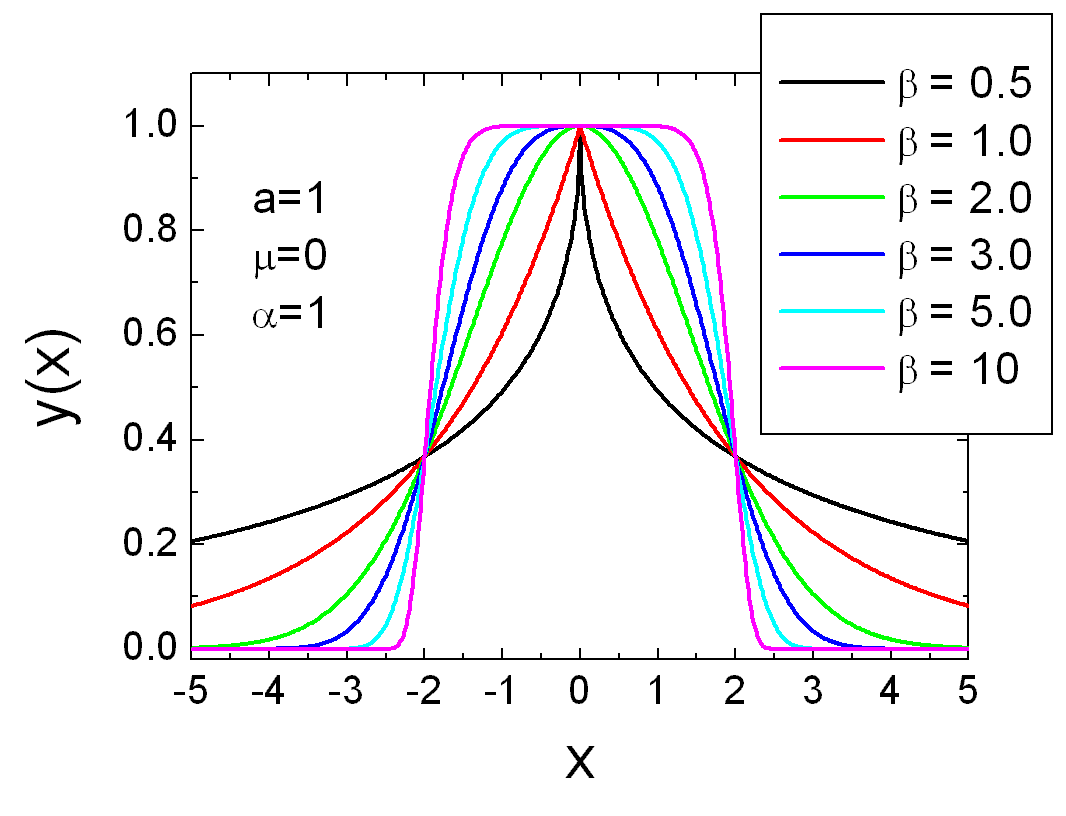
\includegraphics[width=0.768\textwidth]{generalizedGaussian1Amplitude.png}
\end{center}
\caption{Plot of \texttt{generalized Gaussian 1 (Amplitude)}
distribution.} \label{fig:generalizedGaussian1Amplitude}
\end{figure}

\clearpage
\subsection{generalized Gaussian 1 (Area)} ~\\
\label{sec:generalizedGaussian1Area}

\begin{align}
y(x,a,\mu,\alpha,\beta) = a\,
\frac{\beta}{2\alpha\Gamma\left(1/\beta\right)} \,
e^{-\abs{\frac{x-\mu}{\alpha}}^\beta}
\end{align}

\underline{Required parameters:}
\begin{description}
    \item[area] area $a$ below the peak
    \item[center] location parameter (mode) $\mu$
    \item[width] scaling parameter $\alpha \neq 0$
    \item[shape] shape parameter $\beta$
    \item[backgr] offset $c_0$
\end{description}

\underline{Note}
\begin{itemize}
  \item The scaling parameter needs to be positive $(\alpha > 0)$.
  \item Default (size) distribution: Monodisperse
\end{itemize}

\begin{figure}[htb]
\begin{center}
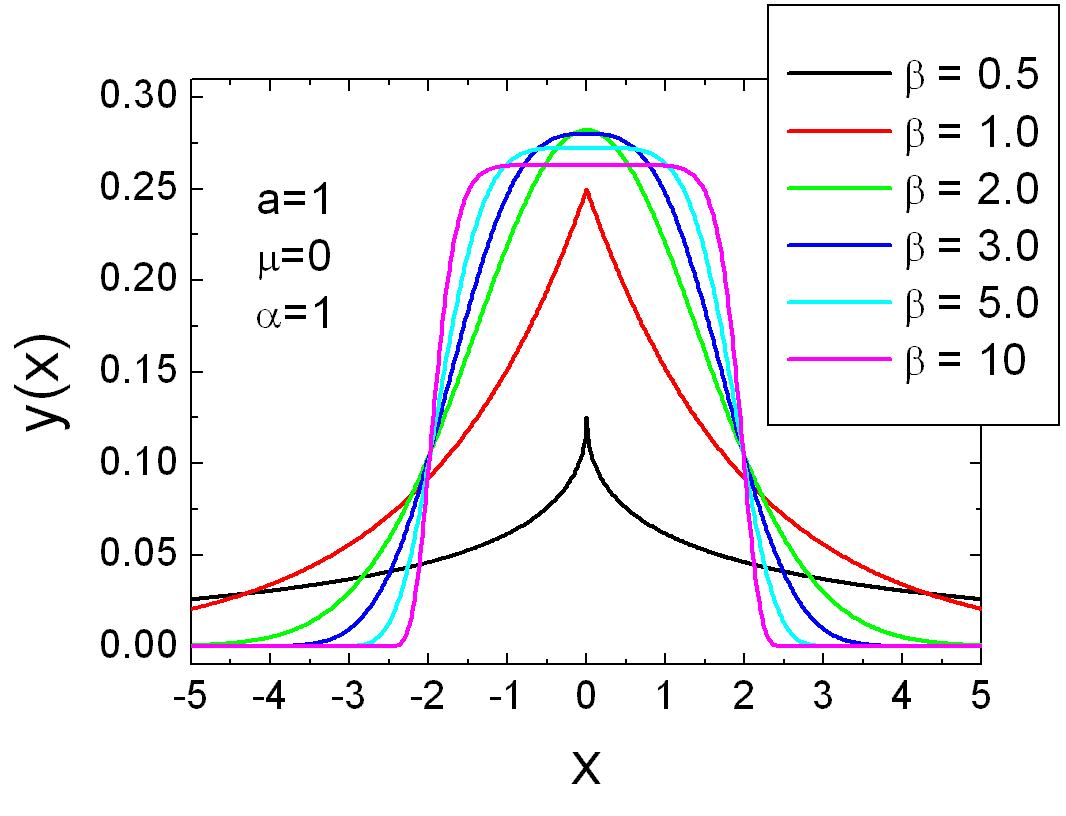
\includegraphics[width=0.768\textwidth]{generalizedGaussian1Area.png}
\end{center}
\caption{Plot of \texttt{generalized Gaussian 1 (Area)}
distribution.} \label{fig:generalizedGaussian1Area}
\end{figure}

%%%%%%%%%%%%%%%%%%%%%%%%%%%%%%%%%%%%%%%%%%%%%%%%%%%%%%%%%%%%%%%%%%%%%%%%%%%%%%%%
\clearpage
\section{generalized Gaussian 2} ~\\
\label{sec:generalizedGaussian2}
\begin{align}
x_\text{mode} & =
\begin{cases} \frac{\alpha}{\kappa} - \frac{\alpha}{\kappa}
e^{-\kappa^2/2} + \xi & \text{ if } \kappa \neq 0 \\
\xi & \text{ if } \kappa = 0 \\
\end{cases}
\end{align}

\clearpage
\subsection{generalized Gaussian 2 (Amplitude)} ~\\
\label{sec:generalizedGaussian2Amplitude}

\begin{align}
y(x) &= A\, \alpha\sqrt{2\pi}\exp\left(-\frac{\kappa^2}{2}\right)
\frac{\phi(u)}{\alpha-\kappa(x-\xi)} + c_0\\
\text{where} & \nonumber \\
u &=
\begin{cases}
- \frac{1}{\kappa} \log \left[ 1-
\frac{\kappa(x-\xi)}{\alpha} \right] & \text{if } \kappa \neq 0 \\
\frac{x-\xi}{\alpha} & \text{if } \kappa=0
\end{cases} \\
\text{where} & \nonumber \\
\phi(x) &= \frac{1}{\sqrt{2\pi}} \exp\left(-\frac{x^2}{2}\right)
\end{align}

\underline{Required parameters:}
\begin{description}
    \item[amplitude] amplitude $A$ of the peak
    \item[location] location parameter $\xi$
    \item[width] scaling parameter $\alpha > 0$
    \item[shape] shape parameter $\kappa$
    \item[backgr] offset $c_0$
\end{description}


\underline{Note}
\begin{itemize}
  \item The scaling parameter needs to be positive $(\alpha > 0)$.
  \item Default (size) distribution: Monodisperse
\end{itemize}

\begin{figure}[htb]
\begin{center}
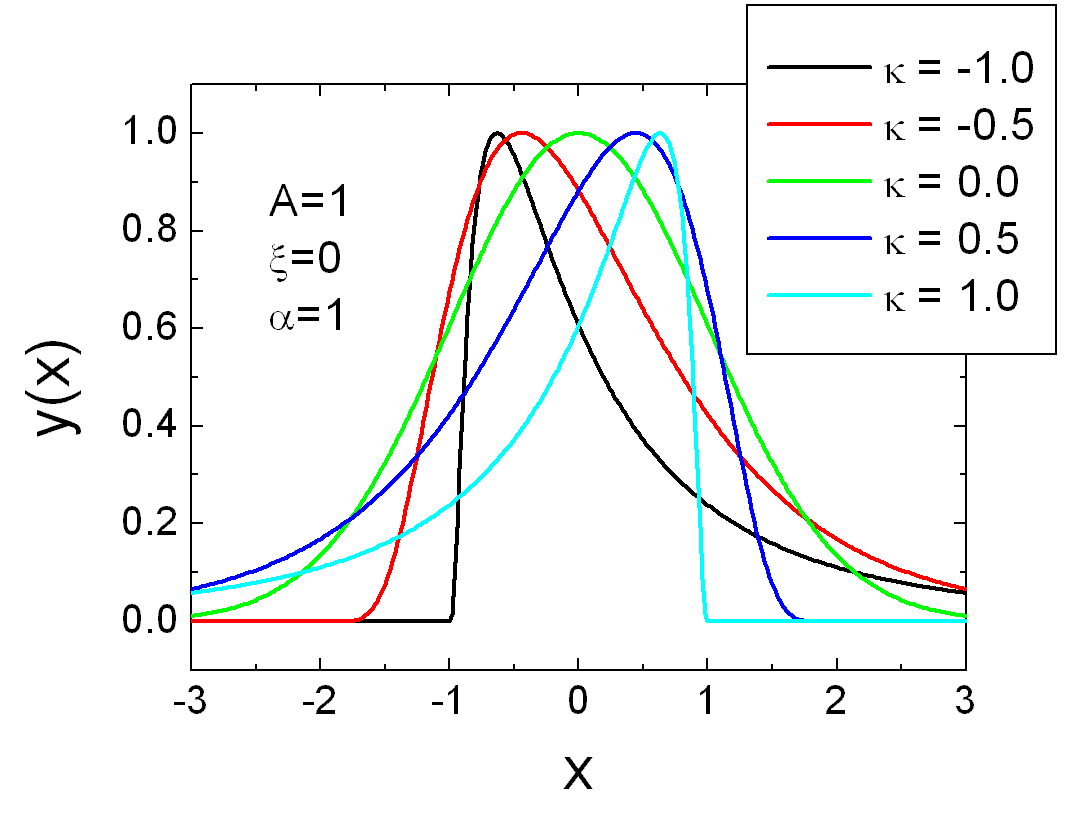
\includegraphics[width=0.768\textwidth]{generalizedGaussian2Amplitude.png}
\end{center}
\caption{Plot of \texttt{generalized Gaussian 2(Amplitude)}
distribution.} \label{fig:generalizedGaussian2Amplitude}
\end{figure}

\clearpage
\subsection{generalized Gaussian 2 (Area)} ~\\
\label{sec:generalizedGaussian2Area}

\begin{subequations}
\begin{align}
y(x) &= A\, \frac{\phi(u)}{\alpha-\kappa(x-\xi)} + c_0\\
\text{where} & \nonumber \\
u &=
\begin{cases}
- \frac{1}{\kappa} \log \left[ 1-
\frac{\kappa(x-\xi)}{\alpha} \right] & \text{if } \kappa \neq 0 \\
\frac{x-\xi}{\alpha} & \text{if } \kappa=0
\end{cases} \\
\text{and} &  \nonumber \\
\phi(u) &= \frac{1}{\sqrt{2\pi}} \exp\left(-\frac{u^2}{2}\right)
\end{align}
\end{subequations}

\underline{Required parameters:}
\begin{description}
    \item[area] area $A$ below the peak
    \item[location] location parameter $\xi$
    \item[width] scaling parameter $\alpha > 0$
    \item[shape] shape parameter $\kappa$
    \item[backgr] offset $c_0$
\end{description}

\underline{Note}
\begin{itemize}
  \item The scaling parameter needs to be positive $(\alpha > 0)$.
  \item Default (size) distribution: Monodisperse
\end{itemize}

\begin{figure}[htb]
\begin{center}
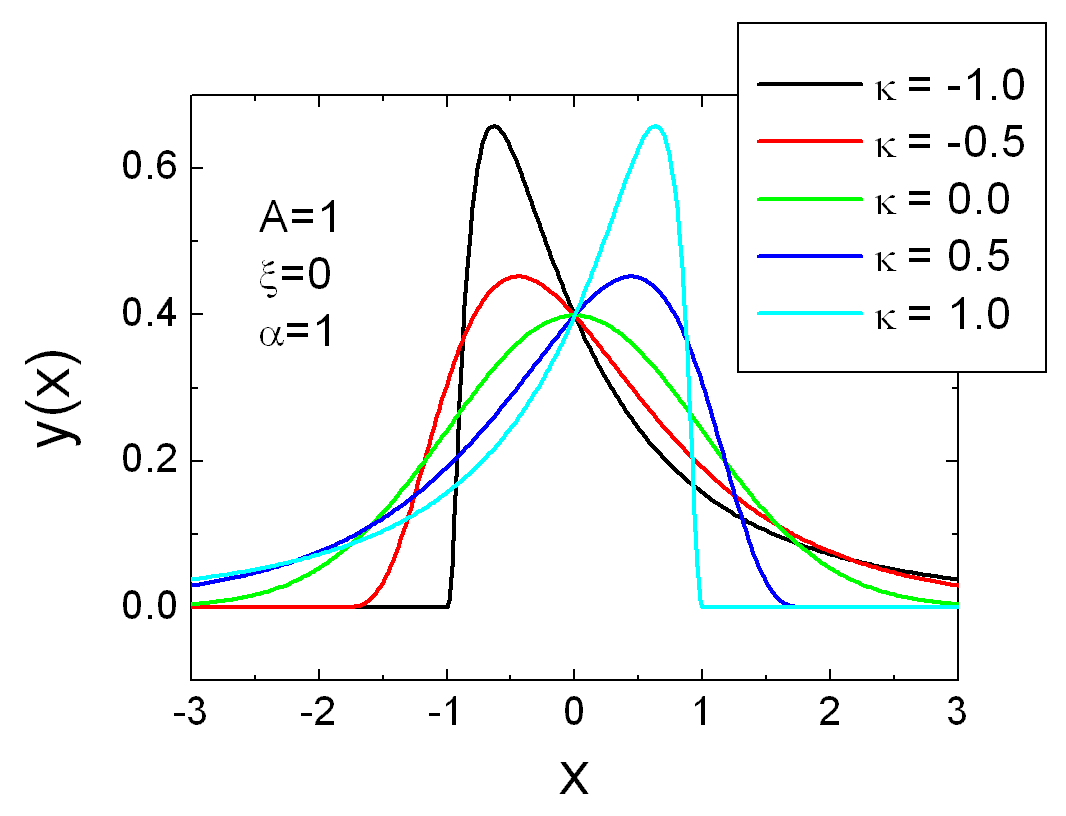
\includegraphics[width=0.768\textwidth]{generalizedGaussian2Area.png}
\end{center}
\caption{Plot of \texttt{generalized Gaussian 2 (Area)}
distribution.} \label{fig:generalizedGaussian2Area}
\end{figure}

%%%%%%%%%%%%%%%%%%%%%%%%%%%%%%%%%%%%%%%%%%%%%%%%%%%%%%%%%%%%%%%%%%%%%%%%%%%%%%%%
\clearpage
\section{Giddings} ~\\
\label{sec:Giddings} The Giddings equation was derived by J. C.
Giddings (Dynamics of Chromatography, Part I, Marcel Decker, New
York, 1965). The equation provides a theoretical description for
chromatographic peaks. The used formulae have been taken from the
Manual of the Peakfit Software package (SeaSolve Software Inc.),
which contains an expression for the for the \texttt{Giddings
(Area)}. As the mode $x_\text{mode}$ of the peak can not be
calculated analytical the amplitude version of this peaks
\texttt{Giddings (Amplitude)} calculates first numerically the mode
of the peak and than normalizes the value at $x_\text{mode}$ to be
$y(x_\text{mode})=A$.

\clearpage
\subsection{Giddings (Amplitude)} ~\\
\label{sec:GiddingsAmplitude} As the mode $x_\text{mode}$ of this
peak can not be calculated analytical this version of the Giddings
peak calculates first numerically the mode of the peak and than
normalizes the value at $x_\text{mode}$ to be $y(x_\text{mode})=A$.

\begin{subequations}
\begin{align}
y(x) & = \frac{A}{c} \sqrt{\frac{\beta}{x}} \,
\mathrm{I}_1\left(\frac{2\sqrt{\beta x}}{\sigma}\right)
\exp\left(-\frac{x+\beta}{\sigma}\right) \\
\text{with } & \nonumber \\
c & = \sqrt{\frac{\beta}{x_\text{mode}}} \,
\mathrm{I}_1\left(\frac{2\sqrt{\beta x_\text{mode}}}{\sigma}\right)
\exp\left(-\frac{x_\text{mode}+\beta}{\sigma}\right)
\end{align}
\end{subequations}

\underline{Required parameters:}
\begin{description}
    \item[amplitude] amplitude $A$ of the peak
    \item[location] location parameter $\beta$
    \item[width] scaling parameter $\sigma > 0$
    \item[backgr] offset $c_0$
\end{description}

\underline{Note}
\begin{itemize}
  \item The scaling parameter needs to be positive $(\sigma > 0)$.
  \item Default (size) distribution: Monodisperse
\end{itemize}

\begin{figure}[htb]
\begin{center}
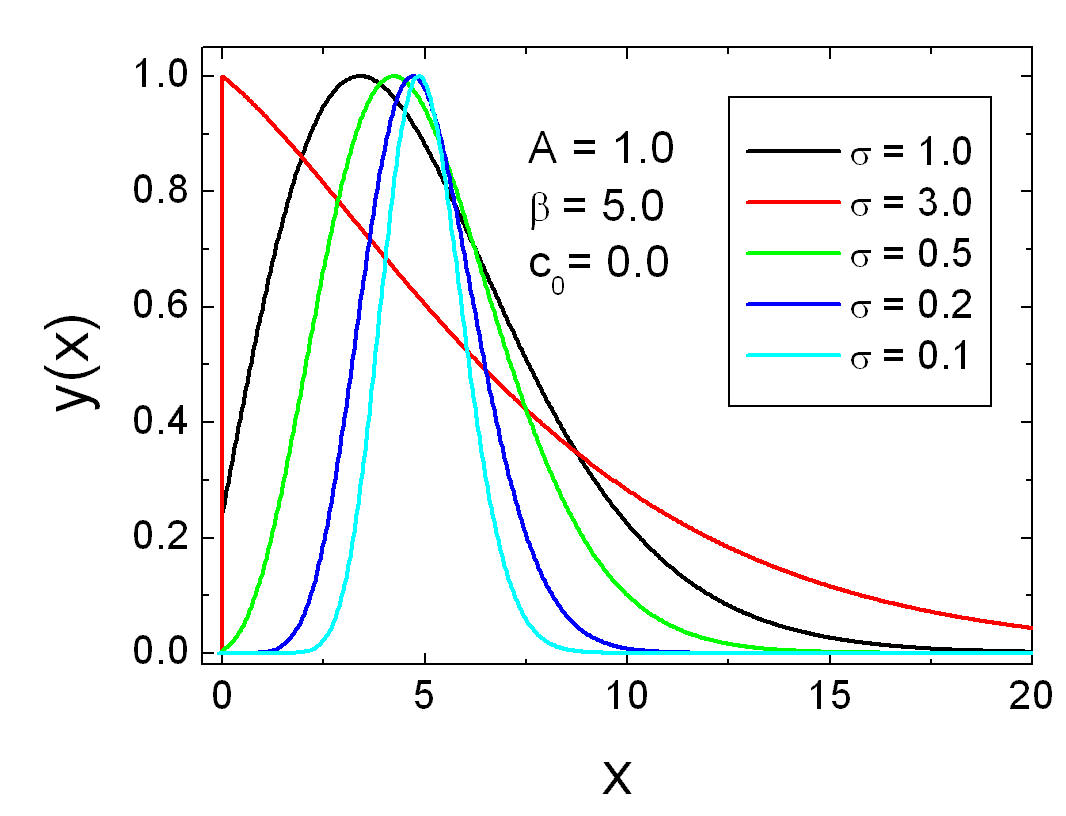
\includegraphics[width=0.768\textwidth]{GiddingsAmplitude.png}
\end{center}
\caption{Plot of \texttt{Giddings (Amplitude)} distribution.}
\label{fig:GiddingsAmplitude}
\end{figure}


\clearpage
\subsection{Giddings (Area)} ~\\
\label{sec:GiddingsArea}
\begin{align}
y(x) & =  \frac{A}{1-\exp\left(-\frac{\beta}{\sigma}\right)} \,
\frac{1}{\sigma} \sqrt{\frac{\beta}{x}} \,
\mathrm{I}_1\left(\frac{2\sqrt{\beta x}}{\sigma}\right)
\exp\left(-\frac{x+\beta}{\sigma}\right)
\end{align}

\underline{Required parameters:}
\begin{description}
    \item[area] area $A$ below the peak
    \item[location] location parameter $\beta$
    \item[width] scaling parameter $\sigma > 0$
    \item[backgr] offset $c_0$
\end{description}

\underline{Note}
\begin{itemize}
  \item The scaling parameter needs to be positive $(\sigma > 0)$.
  \item Default (size) distribution: Monodisperse
\end{itemize}

\begin{figure}[htb]
\begin{center}
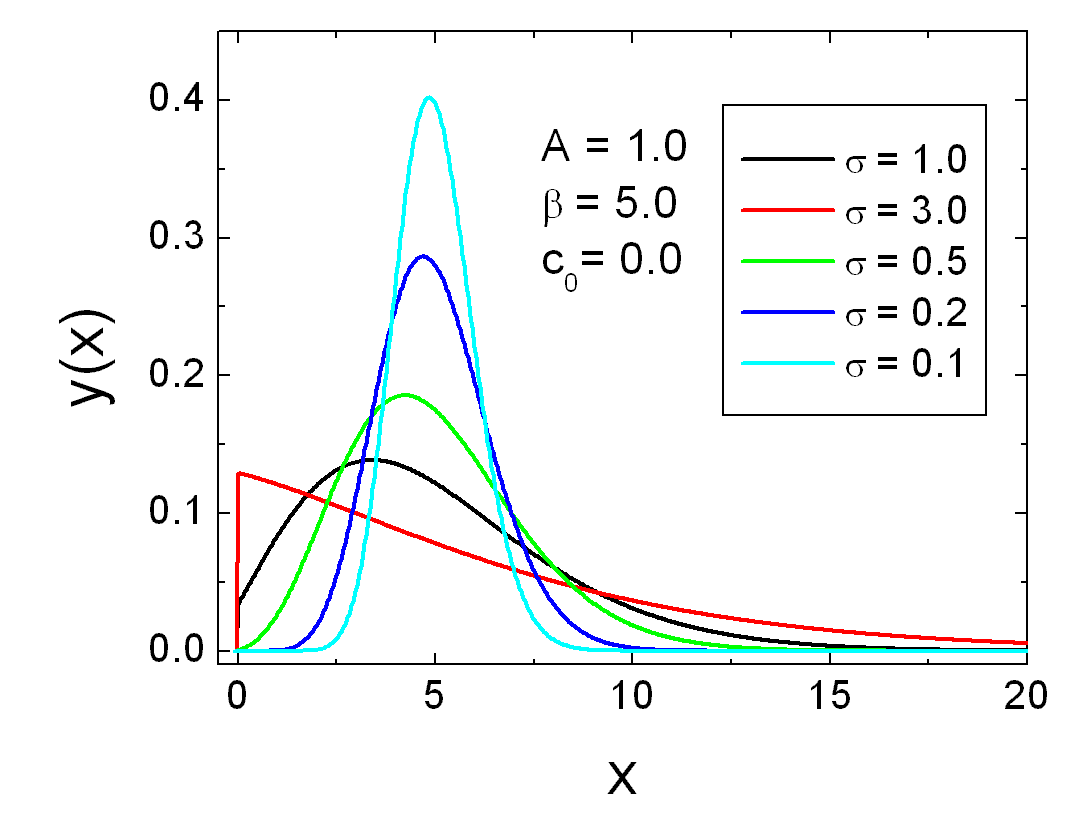
\includegraphics[width=0.768\textwidth]{GiddingsArea.png}
\end{center}
\caption{Plot of \texttt{Giddings (Area)} distribution.}
\label{fig:GiddingsArea}
\end{figure}

%%%%%%%%%%%%%%%%%%%%%%%%%%%%%%%%%%%%%%%%%%%%%%%%%%%%%%%%%%%%%%%%%%%%%%%%%%%%%%%%
\clearpage
\section{Haarhoff - Van der Linde (Area)} ~\\
\label{sec:HaarhoffVanderLindeArea}

\begin{align}
\textrm{HVL}(x) & =
\frac{
       \frac{A\sigma}{\mu\delta\sqrt{2\pi}}
       \exp\left[-\frac{1}{2}\left(\frac{x-\mu}{\sigma}\right)^2\right]
     }{
       \left(\exp\left(\frac{\mu\delta}{\sigma^2}\right)-1\right)^{-1}
       + \frac{1}{2}\left[1+\mathrm{erf}\left(\frac{x-\mu}{\sqrt{2}\sigma}\right)\right]
     }
\end{align}
for $\delta\rightarrow 0$ one get the Gaussian distribution as a limiting case
\begin{align}
\lim_{\delta \rightarrow 0} \textrm{HVL}(x) & =
       \frac{A}{\sigma\sqrt{2\pi}}
       \exp\left[-\frac{1}{2}\left(\frac{x-\mu}{\sigma}\right)^2\right]
\end{align}
as well as for $\mu\rightarrow 0$
\begin{align}
\lim_{\mu \rightarrow 0} \textrm{HVL}(x) & =
       \frac{A}{\sigma\sqrt{2\pi}}
       \exp\left[-\frac{1}{2}\left(\frac{x}{\sigma}\right)^2\right]
\end{align}
\underline{Required parameters:}
\begin{description}
    \item[area] area $A$ below the peak
    \item[width] scaling parameter $\sigma > 0$
    \item[backgr] offset $c_0$
\end{description}

\underline{Note}
\begin{itemize}
  \item The location parameter needs to be positive $(\mu > 0)$.
  \item The scaling parameter needs to be positive $(\sigma > 0)$.
  \item The distortion parameter needs to be nonzero $(\delta \neq 0)$.
  \item Default (size) distribution: Monodisperse
\end{itemize}

\begin{figure}[htb]
\begin{center}
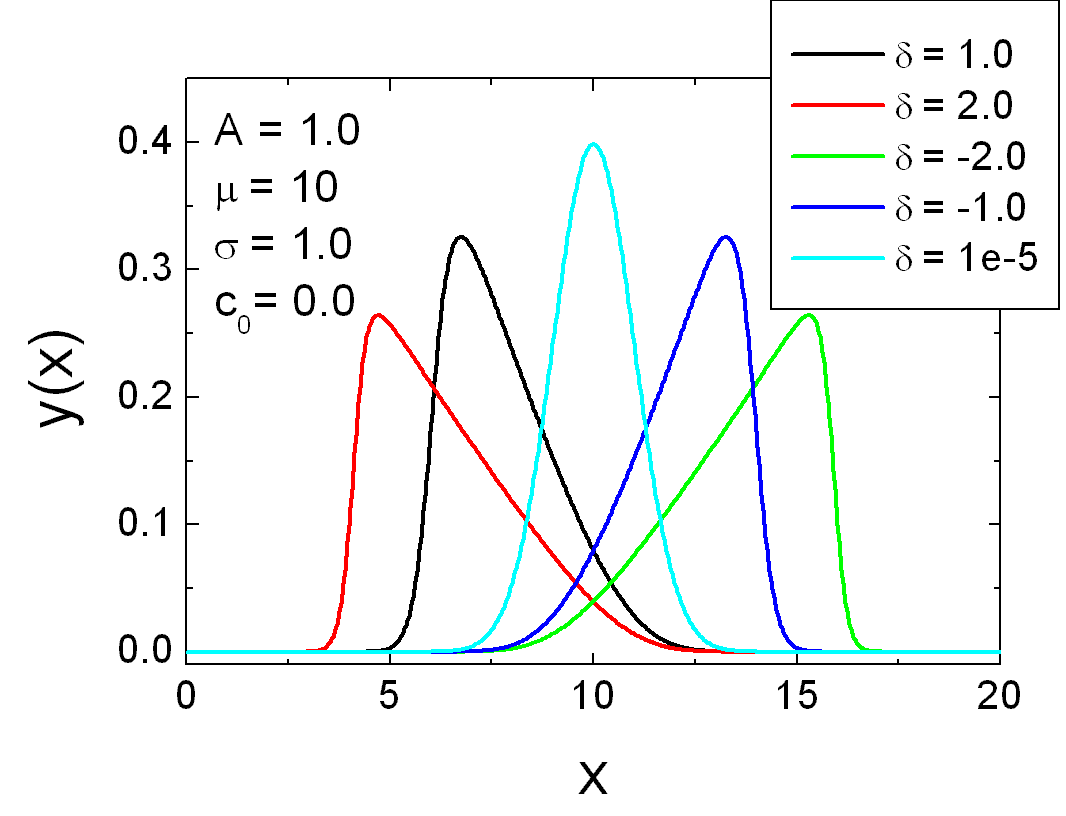
\includegraphics[width=0.768\textwidth]{HaarhoffVanderLindeArea.png}
\end{center}
\caption{Plot of \texttt{HaarhoffVanderLinde (Area)} distribution.}
\label{fig:HaarhoffVanderLindeArea}
\end{figure}


%%%%%%%%%%%%%%%%%%%%%%%%%%%%%%%%%%%%%%%%%%%%%%%%%%%%%%%%%%%%%%%%%%%%%%%%%%%%%%%%
\clearpage
\section{Half Gaussian Modified Gaussian (Area)} ~\\
\label{sec:HalfGaussianModifiedGaussianArea}

The \texttt{Half Gaussian Modified Gaussian (Area)} is the mathematical
convolution of a Gaussian with a half-Gaussian response function. There are only two
components to this model, a primary Gaussian, and a response function
which convolves or smears the Gaussian as in the profiles above. As the
width of the half-Gaussian response increases, peaks become more
asymmetric or tailed. This function directly fit both tailed and fronted peaks. The transition from
tailed to smooth is continuous and occurs at $\delta=0$. The formula has been taken from the
Manual of the Peakfit Software package (SeaSolve Software Inc.).
\begin{align}
y(x) &= A \frac{
            \exp\left(-\frac{1}{2} \frac{\left(x-\mu\right)^2}{\sigma^2+\delta^2}\right)
            \left[1+\mathrm{erf}\left(\frac{\delta \left(x-\mu\right)}{\sqrt{2}\sigma\sqrt{\sigma^2+\delta^2}}\right)\right]
        }{
            \sqrt{2\pi}\sqrt{\sigma^2+\delta^2}}
\end{align}

\underline{Required parameters:}
\begin{description}
    \item[area] area $A$ below the peak
    \item[location] location parameter $\mu$
    \item[width] scaling parameter $\sigma > 0$
    \item[distortion] distortion parameter $\delta \neq 0$
    \item[backgr] offset $c_0$
\end{description}

\underline{Note}
\begin{itemize}
  \item The scaling parameter needs to be positive $(\sigma > 0)$.
  \item The distortion parameter needs to be nonzero $(\delta \neq 0)$.
  \item Default (size) distribution: Monodisperse
\end{itemize}

\begin{figure}[htb]
\begin{center}
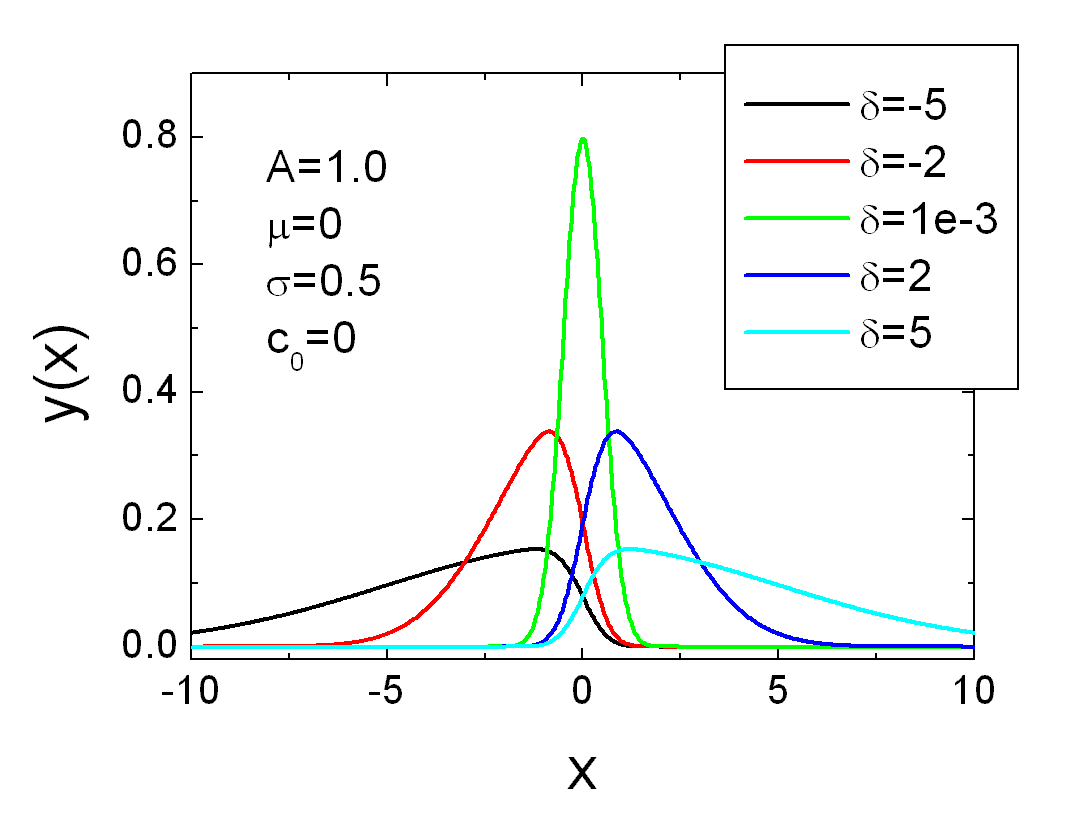
\includegraphics[width=0.768\textwidth]{halfGaussianModifiedGaussianArea.png}
\end{center}
\caption{Plot of \texttt{Half Gaussian Modified Gaussian (Area)} distribution.}
\label{fig:GMGArea}
\end{figure}


%%%%%%%%%%%%%%%%%%%%%%%%%%%%%%%%%%%%%%%%%%%%%%%%%%%%%%%%%%%%%%%%%%%%%%%%%%%%%%%%
\clearpage
\section{Inverted Gamma}
\label{sec:InvertedGamma}

The inverse gamma distribution is a two-parameter family of
continuous probability distributions on the positive real line,
which is the distribution of the reciprocal of a variable
distributed according to the gamma distribution. The inverse gamma
distribution's probability density function is defined over the
support $x > 0$. The probability density function is given by
\begin{align}
p(x) &= \frac{\beta^\alpha}{\Gamma(\alpha)} x^{-\alpha - 1} \exp
\left(\frac{-\beta}{x}\right)
\end{align}
the mode $x_\text{mode}$ of the probabilty function is given by
$x_\text{mode} = \frac{\beta}{\alpha+1}$. The shape parameter
$\alpha$ needs to be positive and non-zero as well as the scale
parameter $\beta$ ($\alpha>0$, $\beta>0$).
The \SASfit version represents a reparametrization of the standard statistical
form. The parameter $\mu$ has been added to enable variable $x$ positioning.
Adjustment terms have been added so that $\mu$ is the mode $x_\text{mode}$.
The function returns $c_0$ for those $x$ where it is undefined.
Note that the amplitude form is much faster.

\clearpage
\subsection{Inverted Gamma (Amplitude)} ~\\
\label{sec:InvertedGammaAmplitude}

\begin{align}
y(x) &= A\frac{\beta\exp\left(\frac{(x-\mu)(\alpha+1)^2}{x(\alpha+1)+\beta-\mu(\alpha+1)}\right)\left(\frac{x(\alpha+1)-\mu(\alpha+1)}{\beta}+1\right)^{-\alpha}}{x(\alpha+1)+\beta-\mu(\alpha+1)}
+c_0
\end{align}

\underline{Required parameters:}
\begin{description}
    \item[amplitude] amplitude $A$ of the peak
    \item[location] location parameter $\mu$
    \item[width] scaling parameter $\beta > 0$
    \item[shape] shape parameter $\alpha > 0$
    \item[backgr] offset $c_0$
\end{description}

\underline{Note}
\begin{itemize}
  \item The scaling parameter needs to be positive $(\beta > 0)$.
  \item The shape parameter needs to be positive $(\alpha > 0)$.
  \item Default (size) distribution: Monodisperse
\end{itemize}

\begin{figure}[htb]
\begin{center}
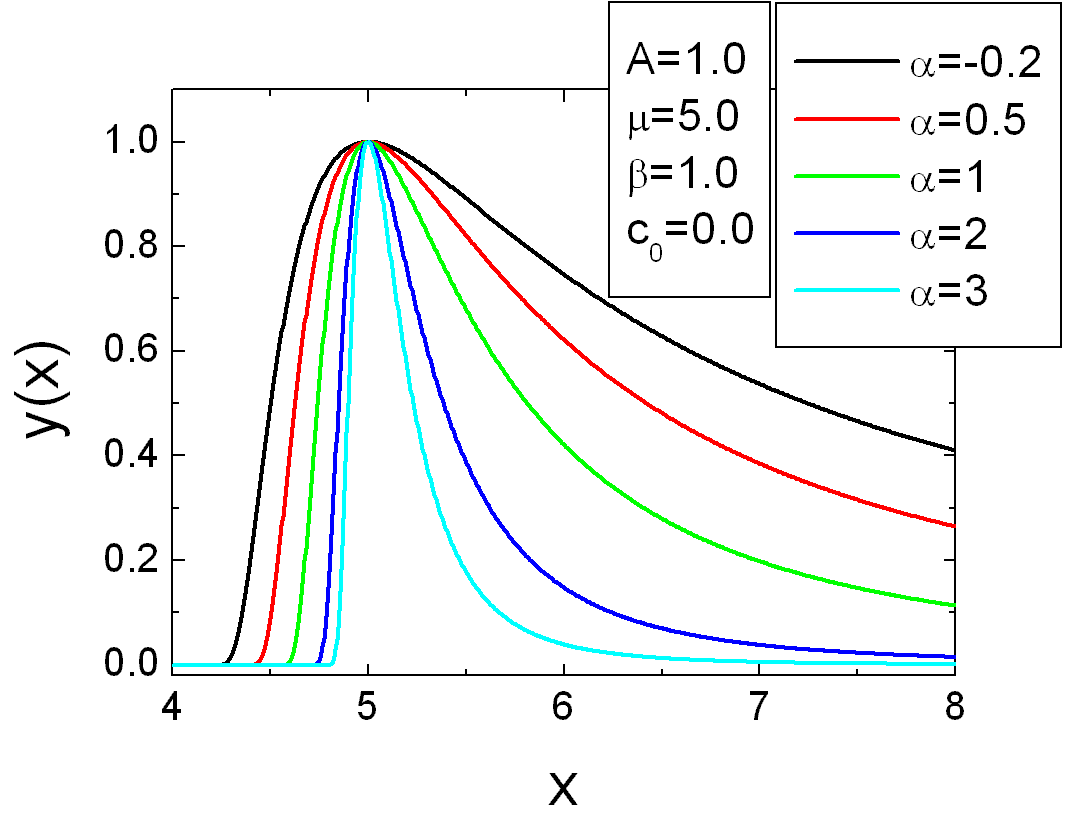
\includegraphics[width=0.768\textwidth]{invertedGammaAmplitude.png}
\end{center}
\caption{Plot of \texttt{inverted Gamma (Amplitude)} distribution.}
\label{fig:invertedGammaAmplitude}
\end{figure}

%%%%%%%%%%%%%%%%%%%%%%%%%%%%%%%%%%%%%%%%%%%%%%%%%%%%%%%%%%%%%%%%%%%%%%%%%%%%%%%%
\clearpage
\subsection{Inverted Gamma (Area)} ~\\
\label{sec:InvertedGammaArea}

\begin{align}
y(x) &= A\frac{(\alpha+1)\exp\left(\frac{\beta(\alpha+1)}{x(\alpha+1)+\beta-\mu(\alpha+1)}\right)\left(\frac{\beta(\alpha+1)}{x(\alpha+1)+\beta-\mu(\alpha+1)}\right)^{\alpha}}{\left(x(\alpha+1)+\beta-\mu(\alpha+1)\right)\Gamma\left(\alpha\right)}
+c_0
\end{align}

\underline{Required parameters:}
\begin{description}
    \item[area] area $A$ below the peak
    \item[location] location parameter $\mu$
    \item[width] scaling parameter $\beta > 0$
    \item[shape] shape parameter $\alpha > 0$
    \item[backgr] offset $c_0$
\end{description}

\underline{Note}
\begin{itemize}
  \item The scaling parameter needs to be positive $(\beta > 0)$.
  \item The shape parameter needs to be positive $(\alpha > 0)$.
  \item Default (size) distribution: Monodisperse
\end{itemize}

\begin{figure}[htb]
\begin{center}
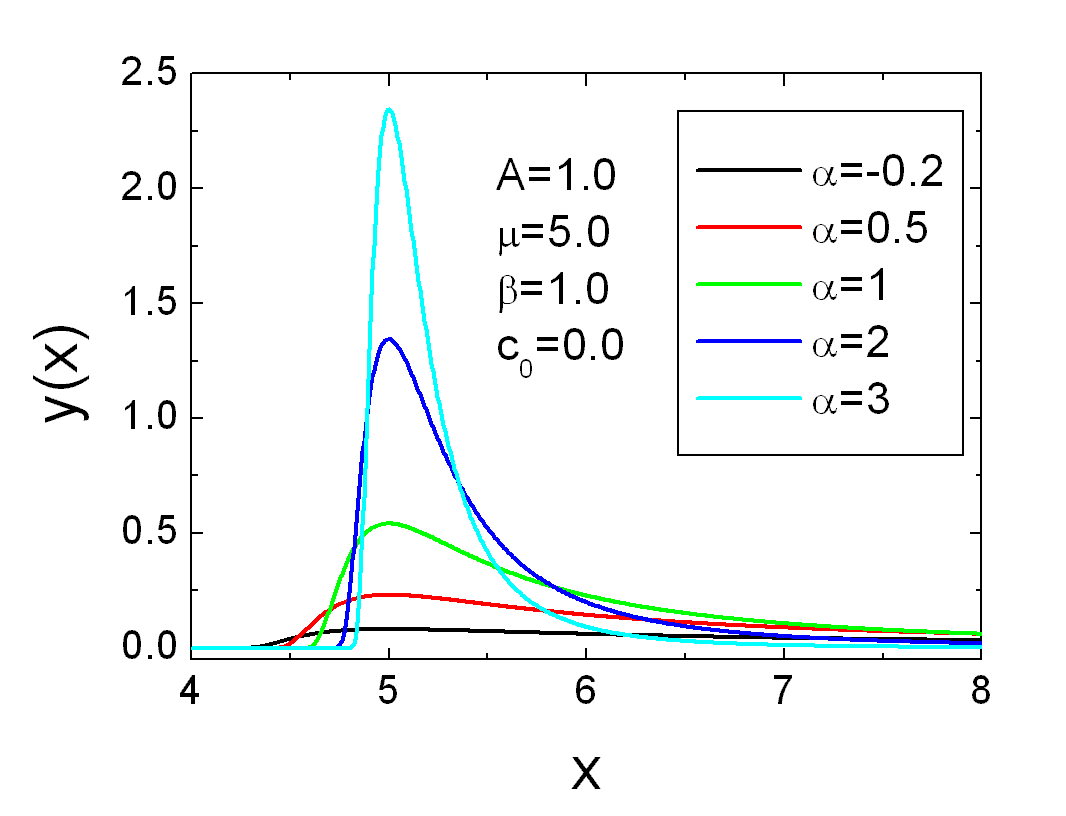
\includegraphics[width=0.768\textwidth]{invertedGammaArea.png}
\end{center}
\caption{Plot of \texttt{inverted Gamma (Area)} distribution.}
\label{fig:invertedGammaArea}
\end{figure}

%%%%%%%%%%%%%%%%%%%%%%%%%%%%%%%%%%%%%%%%%%%%%%%%%%%%%%%%%%%%%%%%%%%%%%%%%%%%%%%%
\clearpage
\section{Kumaraswamy} ~\\
\label{sec:Kumaraswamy}
The Kumaraswamy's double bounded
distribution is a family of continuous probability distributions
defined on the interval $[0,1]$ differing in the values of their two
non-negative shape parameters, $a$ and $b$.
It is similar to the Beta distribution, but much simpler to use
especially in simulation studies due to the simple closed form of
both its probability density function and cumulative distribution
function. The probability density function of the Kumaraswamy distribution is
\begin{align}
p(x; \alpha,\beta) &= \alpha \beta x^{\alpha-1}{ (1-x^\alpha)}^{\beta-1}.
\end{align}
For $\alpha>1$ and $\beta>1$ the mode of the distribution reads as
\begin{align}
x_\text{mode} &= \left(\frac{\alpha-1}{\alpha\beta-1}\right)^{1/\alpha}
\end{align}

\vspace{5mm}
\subsection{Kumaraswamy (Amplitude)} ~\\
\label{sec:KumaraswamyAmplitude}
\begin{align}
y(x) & =
\begin{cases}
\frac{A\alpha \beta \left(\frac{x+x_\text{min}}{x_\text{max}-x_\text{min}}\right)^{\alpha-1}{ \left(1-\left(\frac{x+x_\text{min}}{x_\text{max}-x_\text{min}}\right)^\alpha\right)}^{\beta-1}}{\alpha \beta x_\text{mode}^{\alpha-1}{ (1-x_\text{mode}^\alpha)}^{\beta-1}}
+c_0 & \mbox{for } x \in [x_\text{min},x_\text{max}] \\
c_0 & \mbox{for } x \notin [x_\text{min},x_\text{max}]
\end{cases}
\end{align}

\underline{Required parameters:}
\begin{description}
    \item[ampl.] amplitude $A$ of the Kumaraswamy peak
    \item[xmin] continuous lower boundary parameters $x_\mathrm{min}$
    \item[xmax] continuous upper boundary parameters $x_\mathrm{max}$
    \item[alpha] first shape parameter $\alpha>1$
    \item[beta]  second shape parameter $\beta>1$
    \item[backgr] offset $c_0$
\end{description}

\underline{Note}
\begin{itemize}
  \item Both shape parameter needs to be larger than one $(\alpha,\beta>1)$, as only than
  the distribution has a peak shape.
  \item where the Kumaraswamy distribution is not defined the offset value is returned: \\
  $\forall x\notin (x_\mathrm{min},x_\mathrm{max})\quad y_\mathrm{Beta (ampl)}(x) = c_0$
  \item Default (size) distribution: Monodisperse
\end{itemize}
\begin{figure}[htb]
\begin{center}
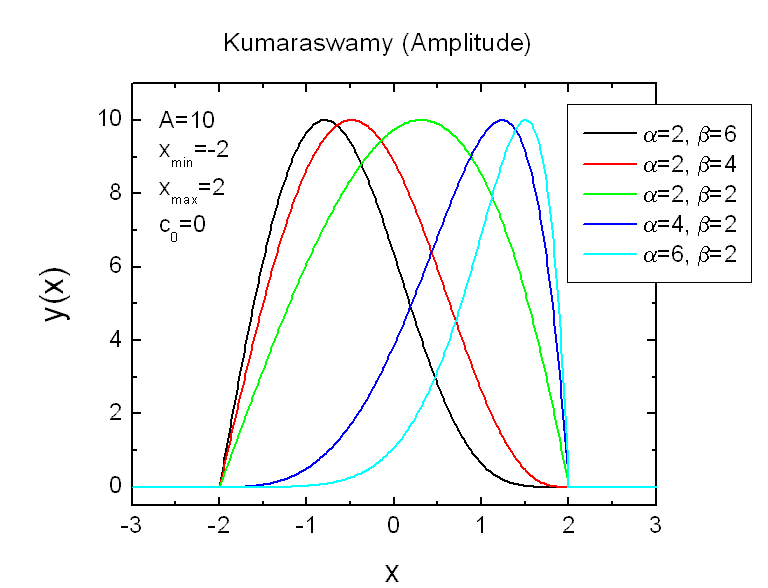
\includegraphics[width=0.768\textwidth]{KumaraswamyAmplitude.png}
\end{center}
\caption{Plot of \texttt{Kumaraswamy (Amplitude)} distribution.}
\label{fig:KumaraswamyAmplitude}
\end{figure}
%%%%%%%%%%%%%%%%%%%%%%%%%%%%%%%%%%%%%%%%%%%%%%%%%%%%%%%%%%%%%%%%%%%%%%%%%%%%%%%%
\clearpage
\section{Kumaraswamy (Area)} ~\\
\label{sec:KumaraswamyArea}
\begin{align}
y(x) & =
\begin{cases}
\frac{A\alpha \beta \left(\frac{x+x_\text{min}}{x_\text{max}-x_\text{min}}\right)^{\alpha-1}{ \left(1-\left(\frac{x+x_\text{min}}{x_\text{max}-x_\text{min}}\right)^\alpha\right)}^{\beta-1}} {x_\text{max}-x_\text{min}}
+c_0 & \mbox{for } x \in [x_\text{min},x_\text{max}] \\
c_0 & \mbox{for } x \notin [x_\text{min},x_\text{max}]
\end{cases}
\end{align}


\underline{Required parameters:}
\begin{description}
    \item[area] area $A$ of the Kumaraswamy distribution
    \item[xmin] continuous lower boundary parameters $x_\mathrm{min}$
    \item[xmax] continuous upper boundary parameters $x_\mathrm{max}$
    \item[alpha] first shape parameter $\alpha>0$
    \item[beta]  second shape parameter $\beta>0$
    \item[backgr] offset $c_0$
\end{description}

\underline{Note}
\begin{itemize}
  \item Both shape parameter needs to be larger than zero $(\alpha,\beta>0)$
  \item where the Kumaraswamy distribution is not defined the offset value is returned: \\
  $\forall x\notin (x_\mathrm{min},x_\mathrm{max})\quad y_\mathrm{Beta (area)}(x) = c_0$
  \item Default (size) distribution: Monodisperse
\end{itemize}

\begin{figure}[htb]
\begin{center}
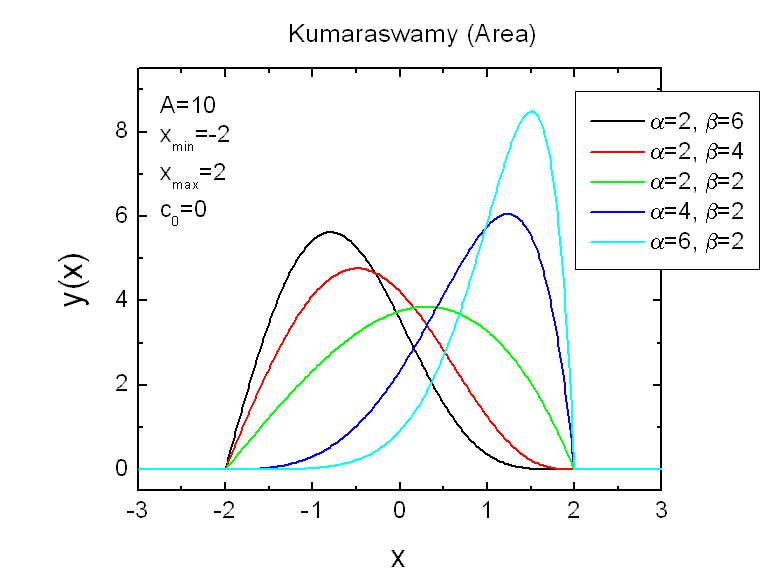
\includegraphics[width=0.768\textwidth]{KumaraswamyArea.png}
\end{center}
\caption{Plot of \texttt{Kumaraswamy (Area)} distribution.}
\label{fig:KumaraswamyArea}
\end{figure}

%%%%%%%%%%%%%%%%%%%%%%%%%%%%%%%%%%%%%%%%%%%%%%%%%%%%%%%%%%%%%%%%%%%%%%%%%%%%%%%%
\clearpage
\section{Laplace} ~\\
\label{sec:Laplace}

A random variable has a Laplace
distribution if its probability density function is
\begin{align}
p(x;x_0,\sigma) &= \frac{1}{2\sigma} \exp \left(
-\frac{\abs{x-x_0}}{\sigma}\right)
\end{align}
Here, $x_0$ is a location parameter and $\sigma > 0$ is a scale
parameter. The Laplace distribution is also sometimes called the
double exponential distribution, because it can be thought of as two
exponential distributions (with an additional location parameter)
spliced together back-to-back, but the term double exponential
distribution is also sometimes used to refer to the Gumbel
distribution.

\vspace{1cm}
\subsection{Laplace (Amplitude)} ~\\
\label{sec:LaplaceAmplitude}
\begin{align}
y(x;x_0,\sigma) &= A \exp \left(
-\frac{\abs{x-x_0}}{\sigma}\right) + c_0
\end{align}


\underline{Required parameters:}
\begin{description}
    \item[amplitude] amplitude $A$ of the Laplace distribution
    \item[center] peak center (mode) $x_0$ of the Laplace distribution
    \item[width] width parameter $\sigma>0$
    \item[backgr] offset $c_0$
\end{description}

\underline{Note}
\begin{itemize}
  \item Width parameter needs to be larger than zero $(\sigma>0)$
  \item Default (size) distribution: Monodisperse
\end{itemize}

\begin{figure}[htb]
\begin{center}
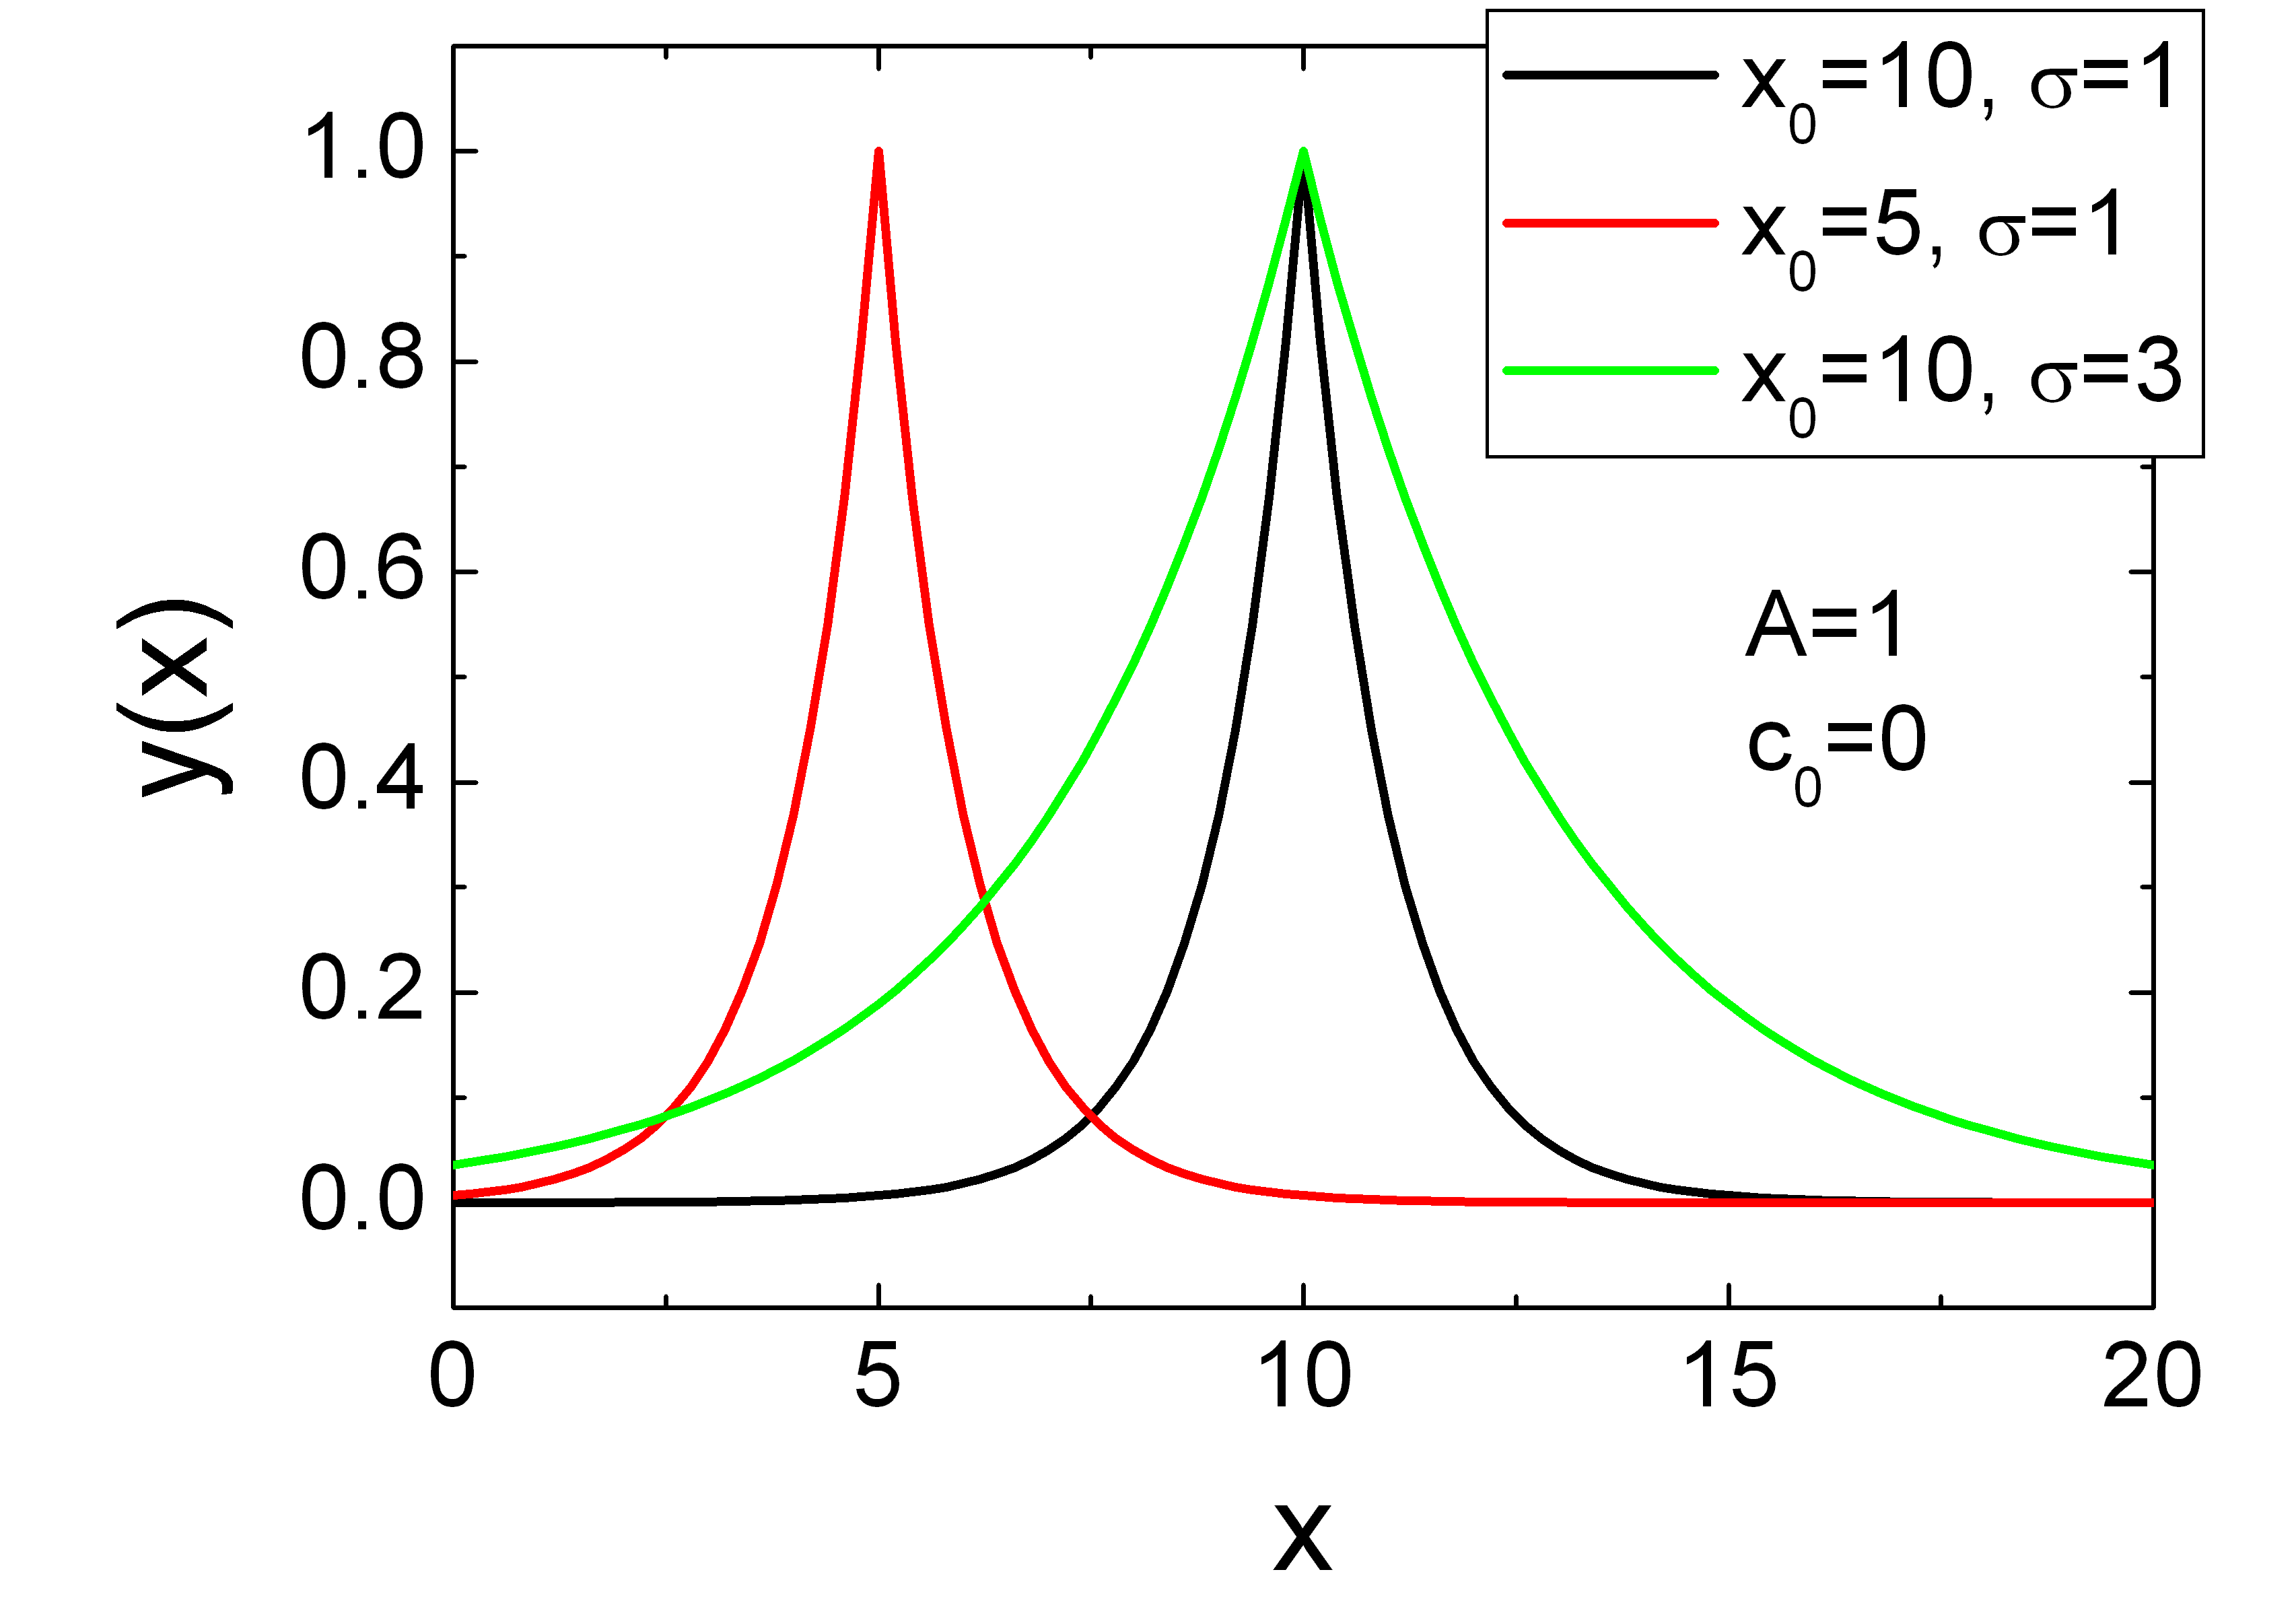
\includegraphics[width=0.6824\textwidth]{LaplaceAmplitude.png}
\end{center}
\caption{Plot of \texttt{Laplace (Amplitude)} distribution.}
\label{fig:LaplaceAmplitude}
\end{figure}

%%%%%%%%%%%%%%%%%%%%%%%%%%%%%%%%%%%%%%%%%%%%%%%%%%%%%%%%%%%%%%%%%%%%%%%%%%%%%%%%
\clearpage
\subsection{Laplace (Area)} ~\\
\label{sec:LaplaceArea}
\begin{align}
y(x;x_0,\sigma) &= \frac{A}{2\sigma} \exp \left(
-\frac{\abs{x-x_0}}{\sigma}\right) + c_0
\end{align}

\underline{Required parameters:}
\begin{description}
    \item[area] area $A$ of the Laplace distribution
    \item[center] peak center (mode) $x_0$ of the Laplace distribution
    \item[width] width parameter $\sigma>0$
    \item[backgr] offset $c_0$
\end{description}

\underline{Note}
\begin{itemize}
  \item Width parameter needs to be larger than zero $(\sigma>0)$
  \item Default (size) distribution: Monodisperse
\end{itemize}


\begin{figure}[htb]
\begin{center}
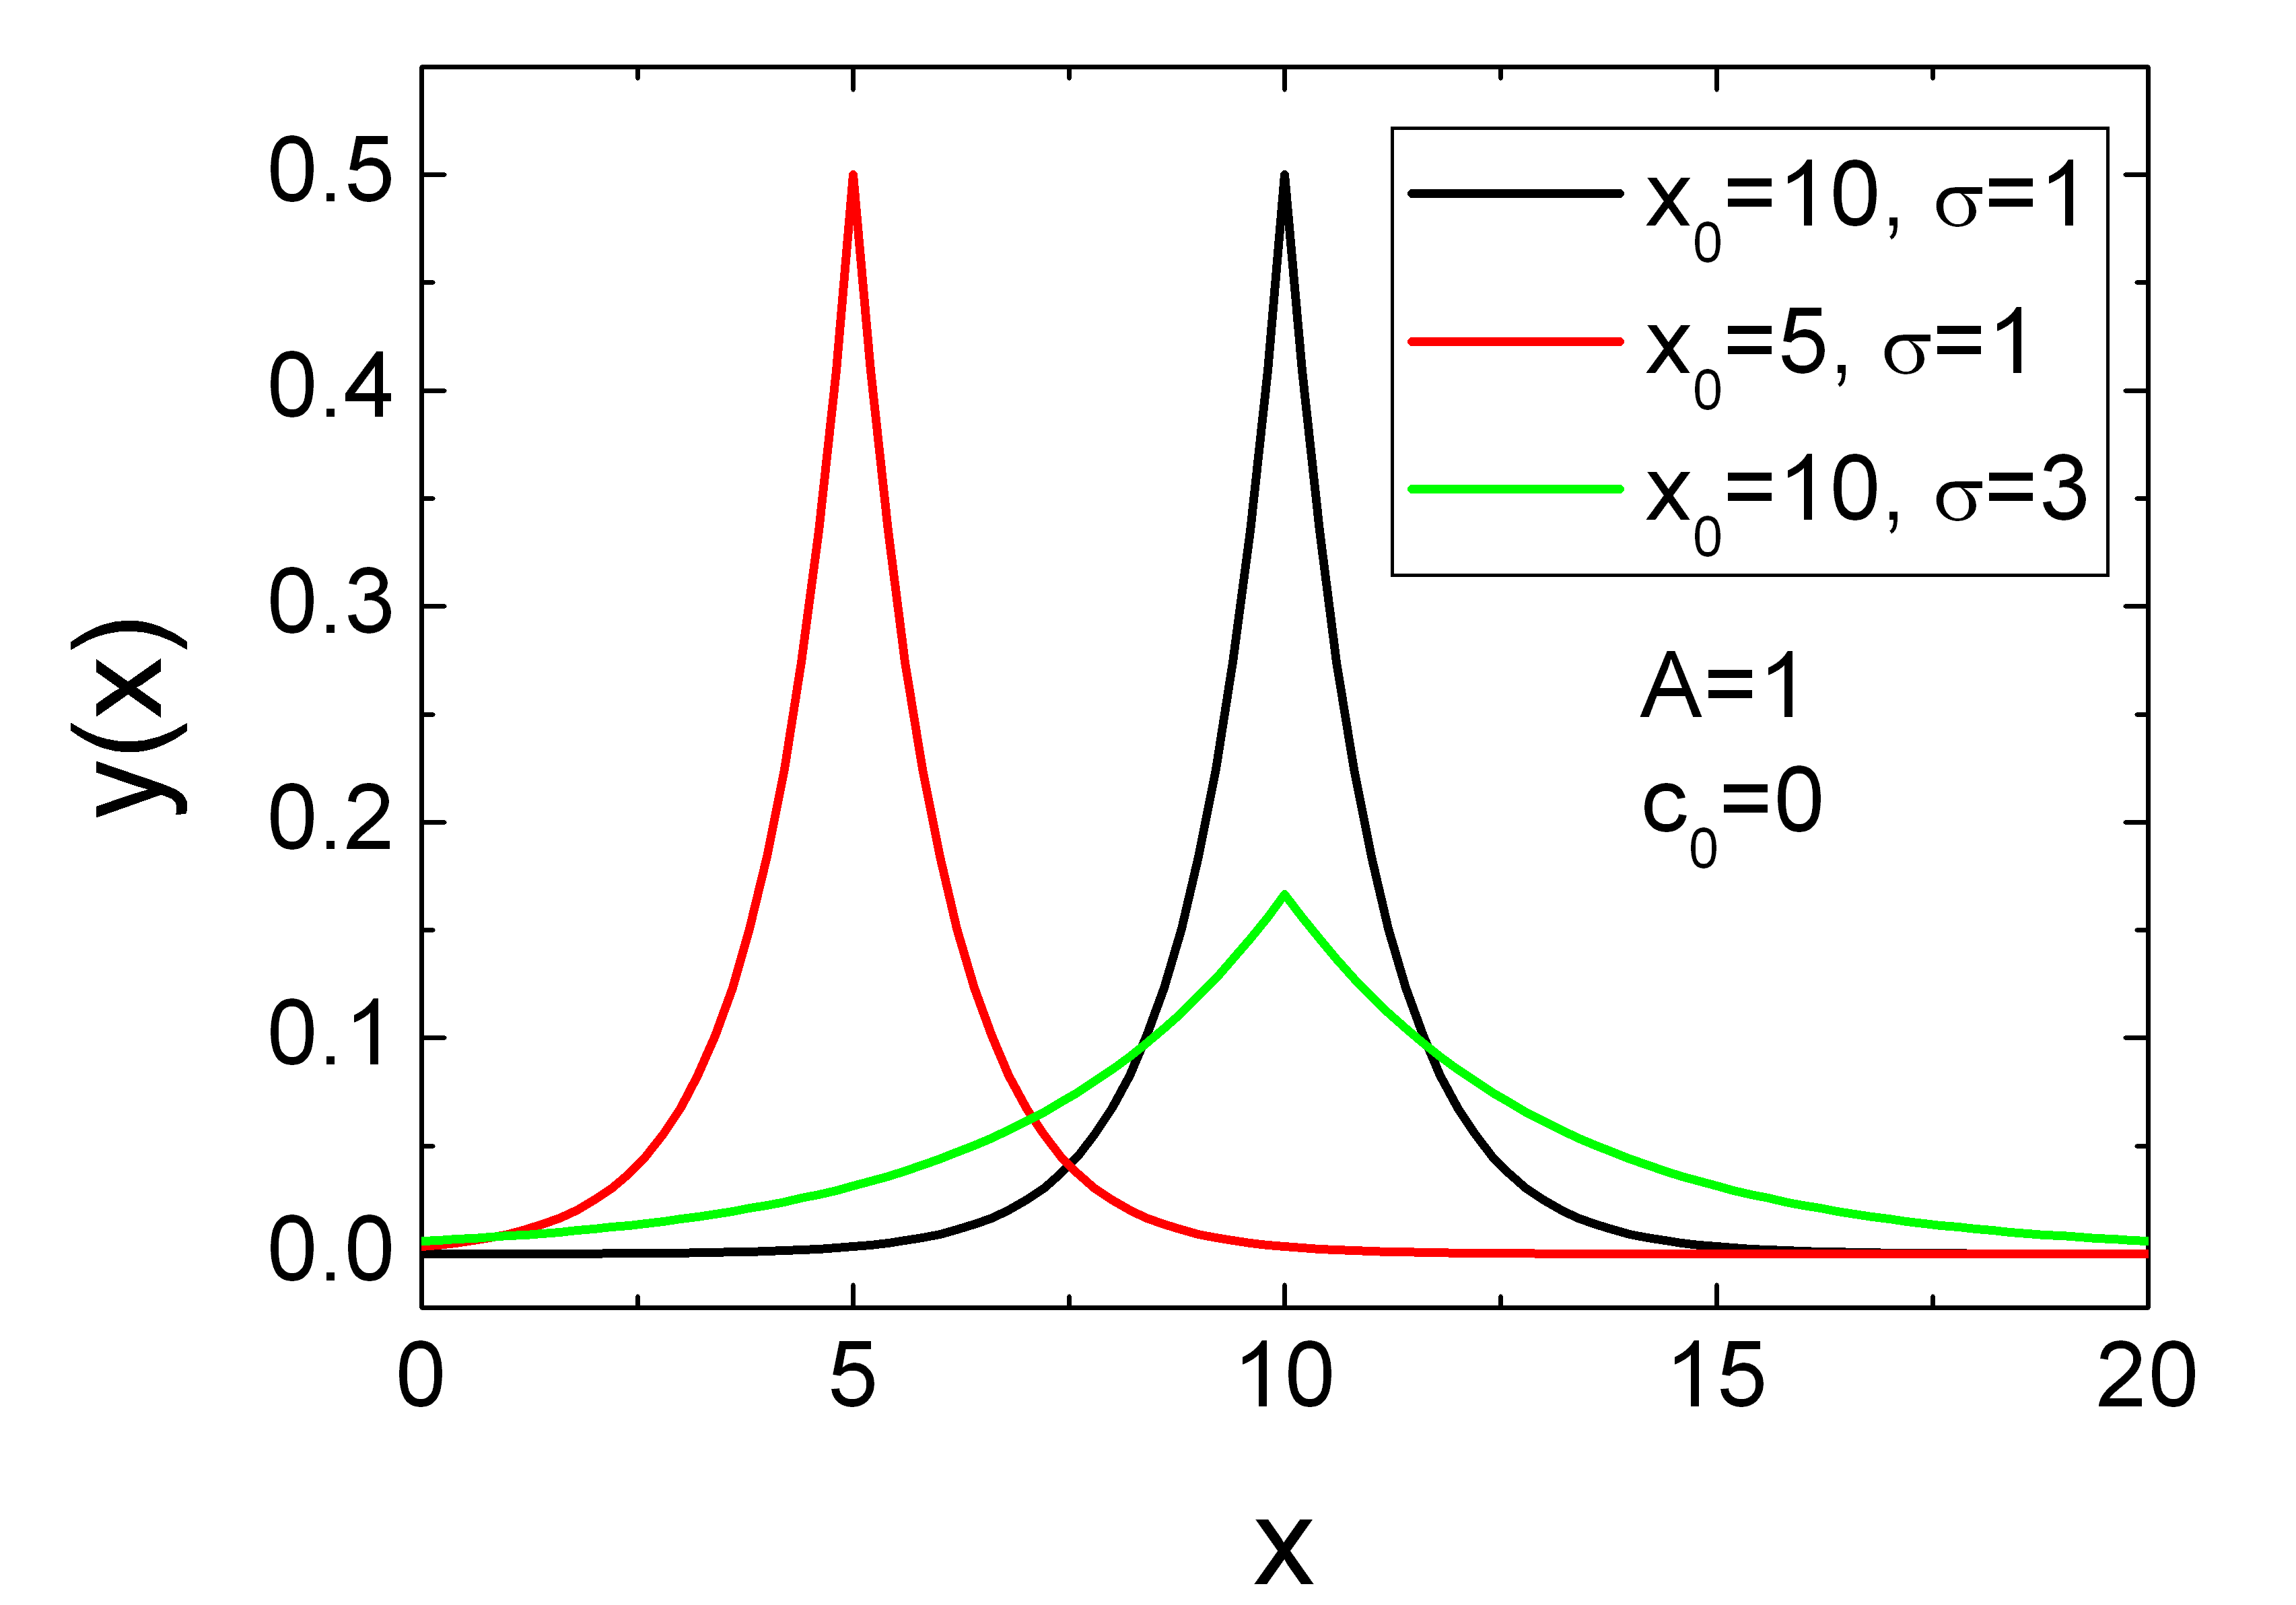
\includegraphics[width=0.6824\textwidth]{LaplaceArea.png}
\end{center}
\caption{Plot of \texttt{Laplace (Area)} distribution.}
\label{fig:LaplaceArea}
\end{figure}

%%%%%%%%%%%%%%%%%%%%%%%%%%%%%%%%%%%%%%%%%%%%%%%%%%%%%%%%%%%%%%%%%%%%%%%%%%%%%%%%
\clearpage
\section{Logistic} ~\\
\label{sec:Logistic}
The logistic distribution is a continuous
probability distribution. It resembles the normal distribution in
shape but has heavier tails (higher kurtosis). The probability
density function (pdf) of the logistic  distribution is given by:
\begin{align}
p(x; x_0,\sigma) &= \frac{\exp\left(-\frac{x-x_0}{\sigma}\right)} {\sigma\left(1+\exp\left(-\frac{x-x_0}{\sigma}\right)\right)^2}
            =\frac{1}{4\,\sigma} \;\operatorname{sech}^2\!\left(\frac{x-x_0}{2\,\sigma}\right).
\end{align}
Because the pdf can be expressed in terms of the square of the
hyperbolic secant function $\operatorname{sech}$, it is sometimes referred to as
the sech-squared distribution. The mode, mean and median values are $x_0$.
\vspace{1cm}
\subsection{Logistic (Amplitude)} ~\\
\label{sec:LogisticAmplitude}
\begin{align}
y(x; x_0,\sigma) &= 4A\frac{\exp\left(-\frac{x-x_0}{\sigma}\right)} {\left(1+\exp\left(-\frac{x-x_0}{\sigma}\right)\right)^2}
\end{align}

\underline{Required parameters:}
\begin{description}
    \item[amplitude] amplitude $A$ of the Logistic distribution
    \item[x0] location parameter (mode) $x_0$
    \item[sigma] width parameters $\sigma$
    \item[backgr] offset $c_0$
\end{description}

\underline{Note}
\begin{itemize}
  \item the width parameter needs to be larger than zero $\sigma > 0$
  \item Default (size) distribution: Monodisperse
\end{itemize}

\begin{figure}[htb]
\begin{center}
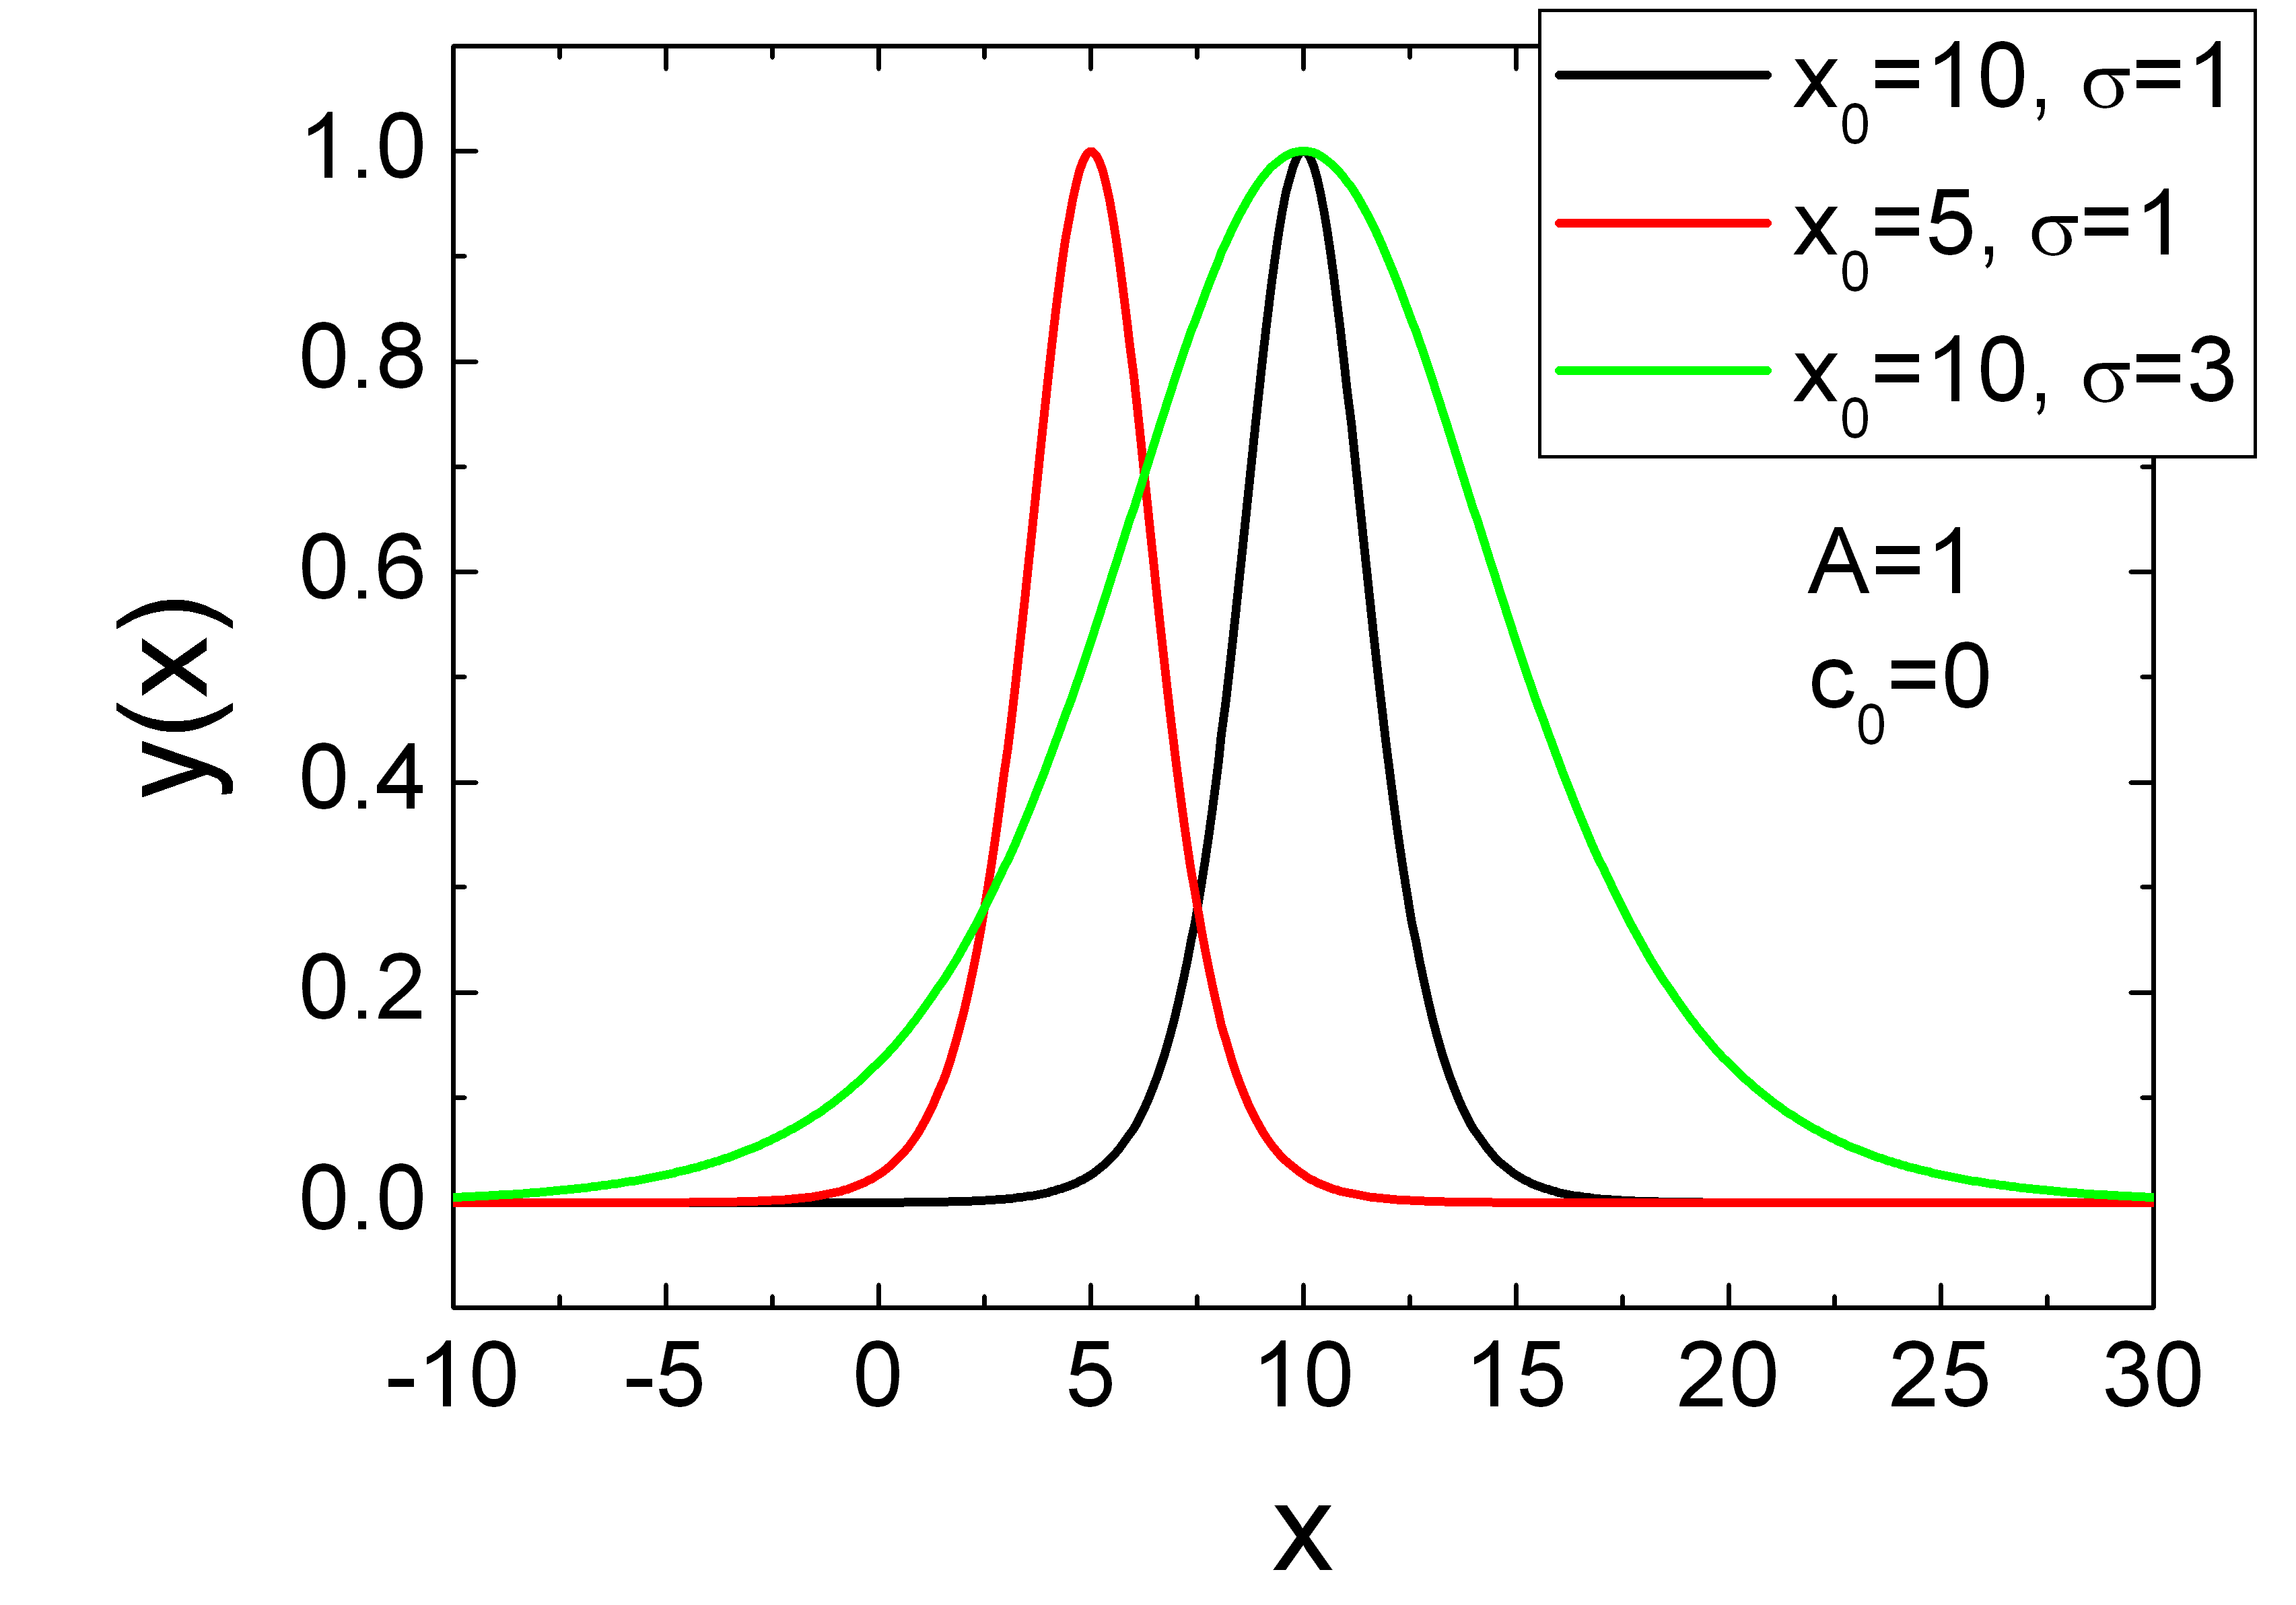
\includegraphics[width=0.6824\textwidth]{LogisticAmplitude.png}
\end{center}
\caption{Plot of \texttt{Logistic (Amplitude)} distribution.}
\label{fig:LogisticAmplitude}
\end{figure}

%%%%%%%%%%%%%%%%%%%%%%%%%%%%%%%%%%%%%%%%%%%%%%%%%%%%%%%%%%%%%%%%%%%%%%%%%%%%%%%%
\clearpage
\subsection{Logistic (Area)} ~\\
\label{sec:LogisticArea}
\begin{align}
y(x; x_0,\sigma) &= A\; \frac{\exp\left(-\frac{x-x_0}{\sigma}\right)} {\sigma\left(1+\exp\left(-\frac{x-x_0}{\sigma}\right)\right)^2}
\end{align}

\underline{Required parameters:}
\begin{description}
    \item[area] area $A$ of the Logistic distribution
    \item[x0] location parameter (mode) $x_0$
    \item[sigma] width parameters $\sigma$
    \item[backgr] offset $c_0$
\end{description}

\underline{Note}
\begin{itemize}
  \item the width parameter needs to be larger than zero $\sigma > 0$
  \item Default (size) distribution: Monodisperse
\end{itemize}

\begin{figure}[htb]
\begin{center}
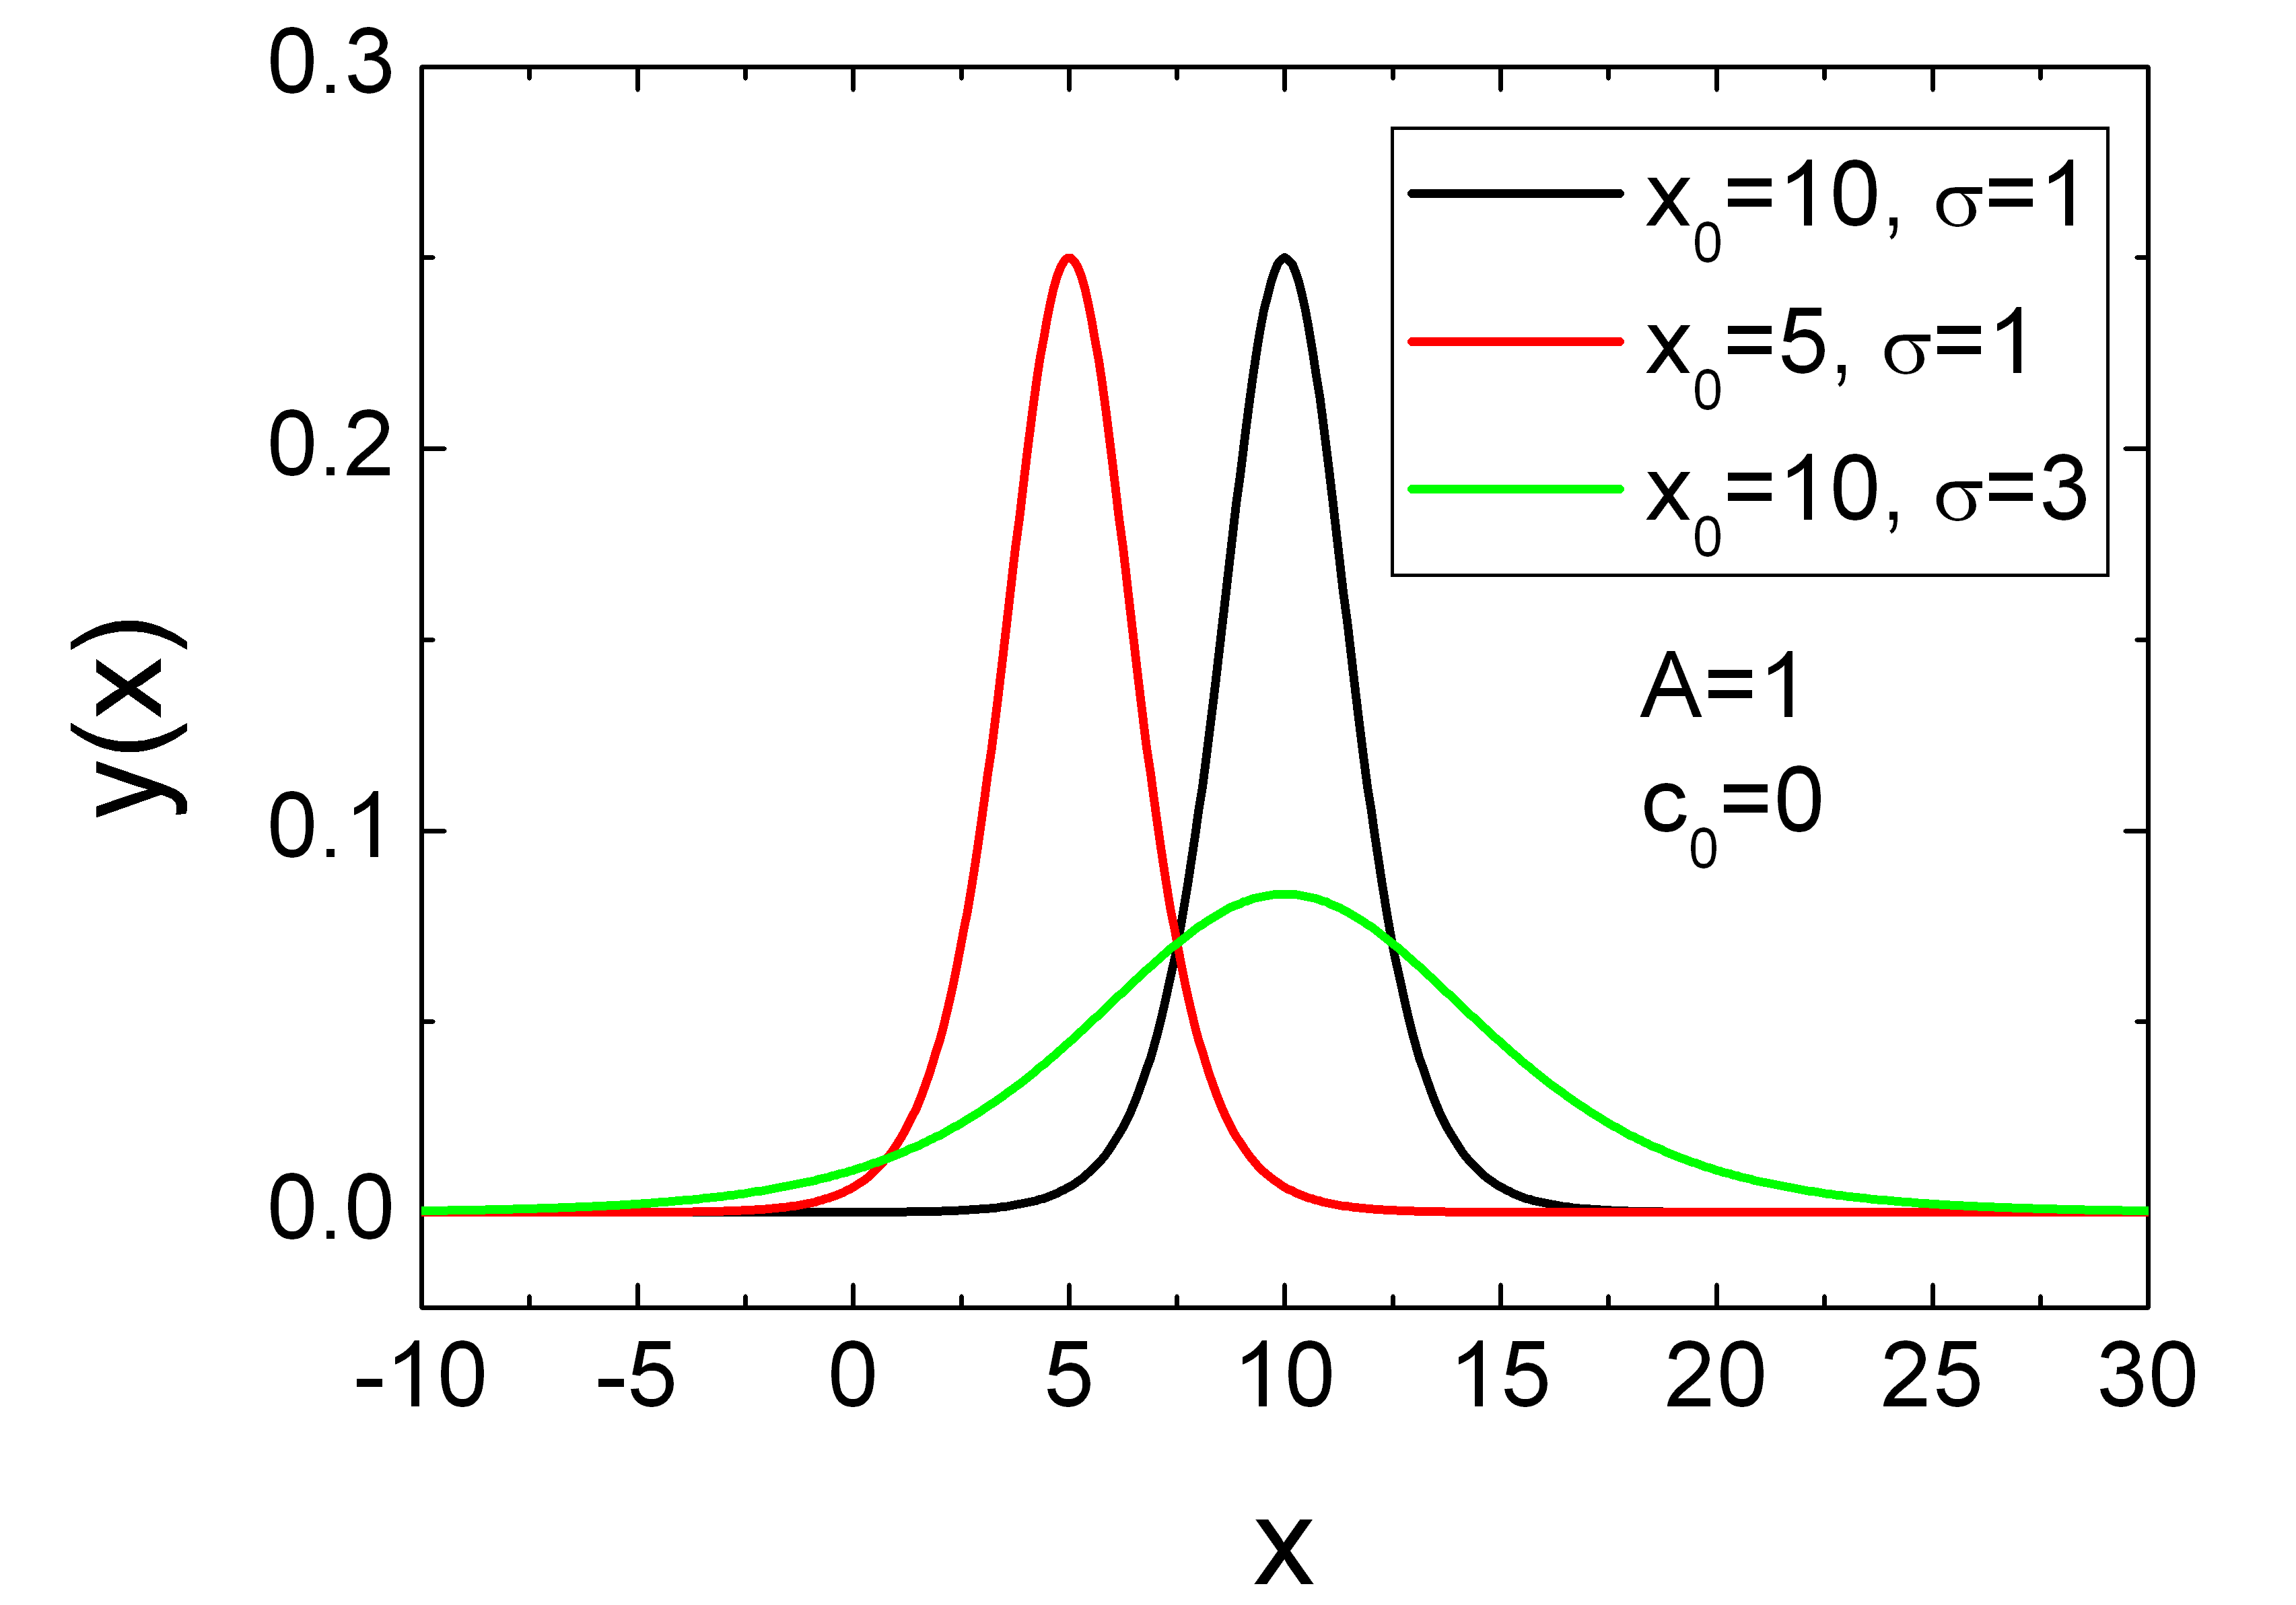
\includegraphics[width=0.6824\textwidth]{LogisticArea.png}
\end{center}
\caption{Plot of \texttt{Logistic (Area)} distribution}.
\label{fig:LogisticArea}
\end{figure}

%%%%%%%%%%%%%%%%%%%%%%%%%%%%%%%%%%%%%%%%%%%%%%%%%%%%%%%%%%%%%%%%%%%%%%%%%%%%%%%%
\clearpage
\section{LogLogistic} ~\\
\label{sec:LogLogistic}
As may be indicated by the name, the loglogistic (known as the Fisk distribution in economics)
distribution has certain similarities to the logistic distribution. A random variable
is loglogistically distributed if the logarithm of the random variable is logistically distributed.
The \texttt{LogLogistic} distribution is a two-parameter distribution with parameters
$\sigma$ and $x_0$. It is similar in shape to the log-normal distribution but has heavier tails.

The pdf for this distribution is given by:
\begin{align}
p(x;\mu,\sigma) &=\frac{\exp\left(-\frac{\log\left(x\right)-\log(\mu)}{\sigma}\right)}{\sigma \left(x\right)\left(1+\exp\left(-\frac{\log(x)-\log(\mu)}{\sigma}\right)\right)^2}
= \frac{ \left(\frac{x}{\mu}\right)^{-1/\sigma} } { x\sigma\left[ 1+\left(\frac{x}{\mu}\right)^{-1/\sigma} \right]^2 }.
\end{align}
where $0 < x < \infty$, $-\infty < x_0 < \infty$ and $0 < \sigma < \infty$.
The mode of the \texttt{LogLogistic} distribution, if $\sigma < 1$, is given by:
\begin{align}
\mathrm{mode} &= \mu\left(\frac{1-\sigma}{1+\sigma}\right)^{\sigma}
\end{align}

\vspace{1cm}

\subsection{LogLogistic (Amplitude)} ~\\
\label{sec:LogLogisticAmplitude}
\begin{align}
y(x) &=
\begin{cases}
A \frac{ \left(\frac{x-x_0}{\mu}\right)^{-1/\sigma} } { \left(x-x_0\right)\sigma\left[ 1+\left(\frac{x-x_0}{\mu}\right)^{-1/\sigma} \right]^2 } +c_0 & \mbox{for } x \geq x_0\\
c_0 & \mbox{for } x<x_0
\end{cases}
\end{align}

\underline{Required parameters:}
\begin{description}
    \item[amplitude] amplitude $A$ of the LogLogistic distribution
    \item[x0] location parameter $x_0$
    \item[mu] scale parameter $\mu$
    \item[sigma] shape parameters $\sigma$
    \item[backgr] offset $c_0$
\end{description}

\underline{Note}
\begin{itemize}
  \item the width parameter needs to be larger than zero $0<\sigma <1$
  \item Default (size) distribution: Monodisperse
\end{itemize}


\begin{figure}[htb]
\begin{center}
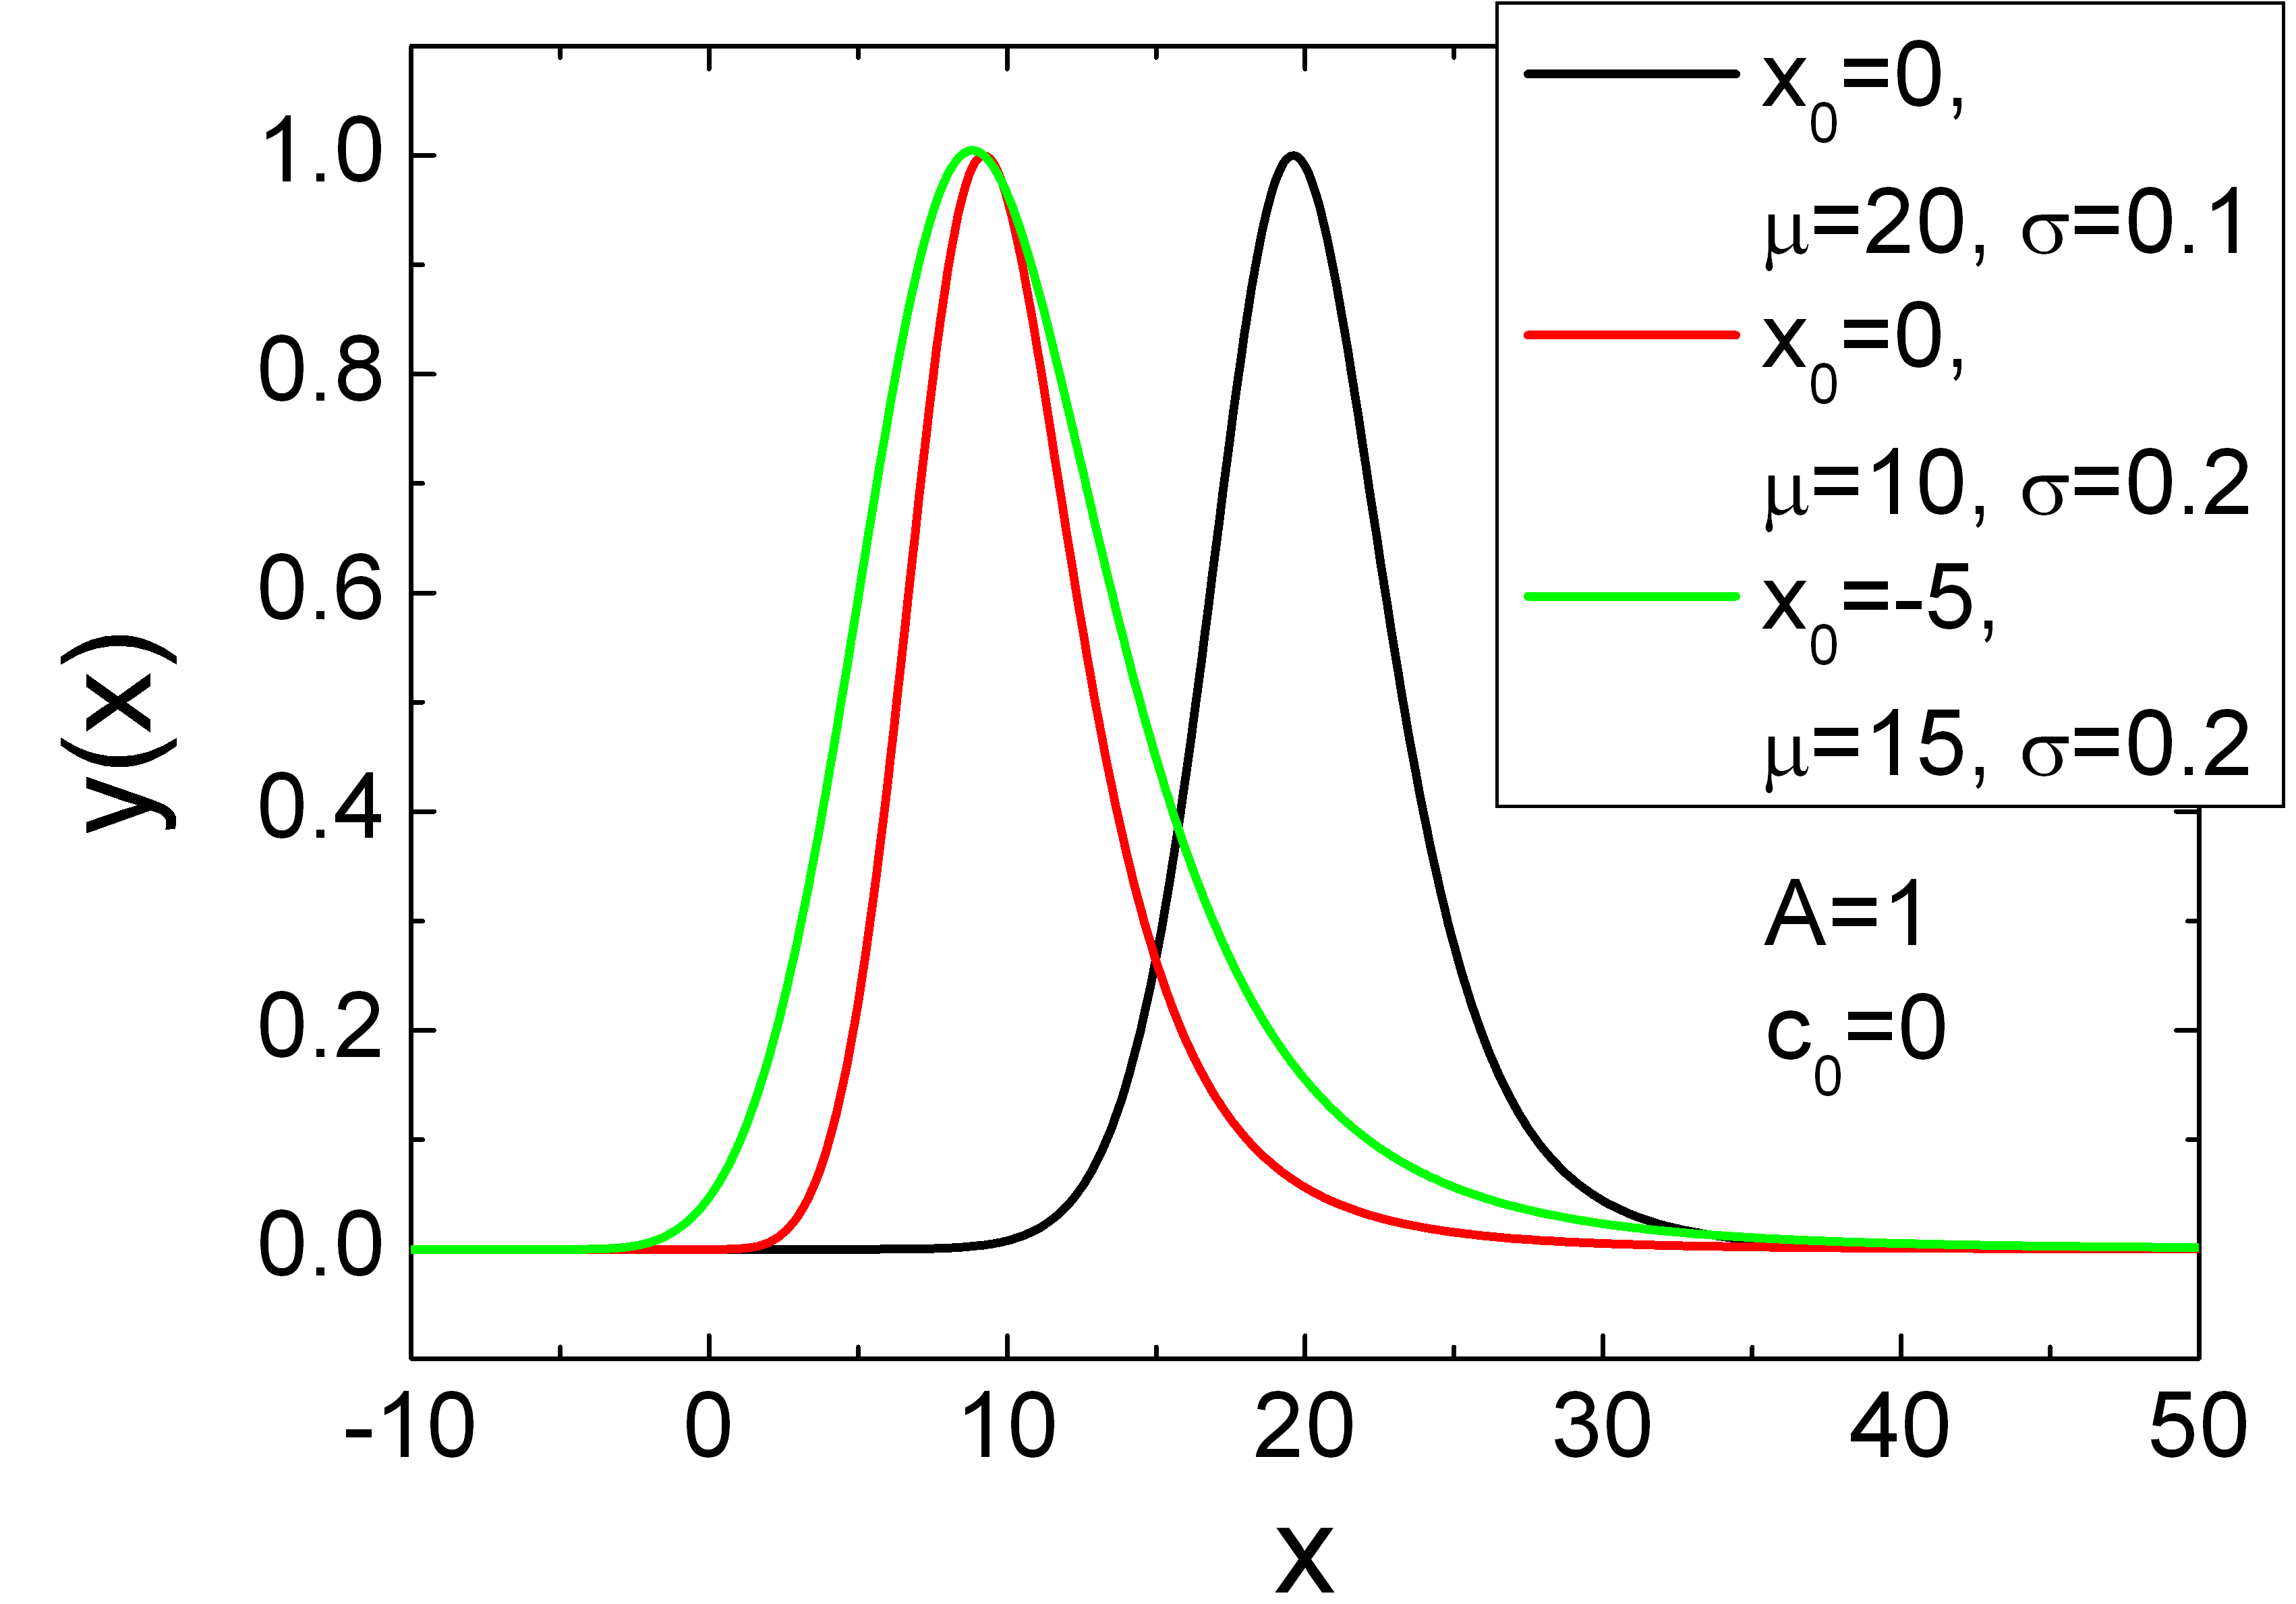
\includegraphics[width=0.6824\textwidth]{LogLogisticAmplitude.png}
\end{center}
\caption{Plot of \texttt{LogLogistic (Amplitude)} distribution.}
\label{fig:LogLogisticAmplitude}
\end{figure}

%%%%%%%%%%%%%%%%%%%%%%%%%%%%%%%%%%%%%%%%%%%%%%%%%%%%%%%%%%%%%%%%%%%%%%%%%%%%%%%%
\clearpage
\subsection{LogLogistic (Area)} ~\\
\label{sec:LogLogisticArea}
\begin{align}
y(x) &= A \frac{ \left(\frac{x}{x_0}\right)^{-1/\sigma} } { x\sigma\left[ 1+\left(\frac{x}{x_0}\right)^{-1/\sigma} \right]^2 }.
\end{align}

\underline{Required parameters:}
\begin{description}
    \item[area] area $A$ of the LogLogistic distribution
    \item[x0] location parameter $x_0$
    \item[mu] scale parameter $\mu$
    \item[sigma] shape parameters $0 < \sigma < 1$
    \item[backgr] offset $c_0$
\end{description}

\underline{Note}
\begin{itemize}
  \item the width parameter needs to be larger than zero $\sigma > 0$
  \item Default (size) distribution: Monodisperse
\end{itemize}


\begin{figure}[htb]
\begin{center}
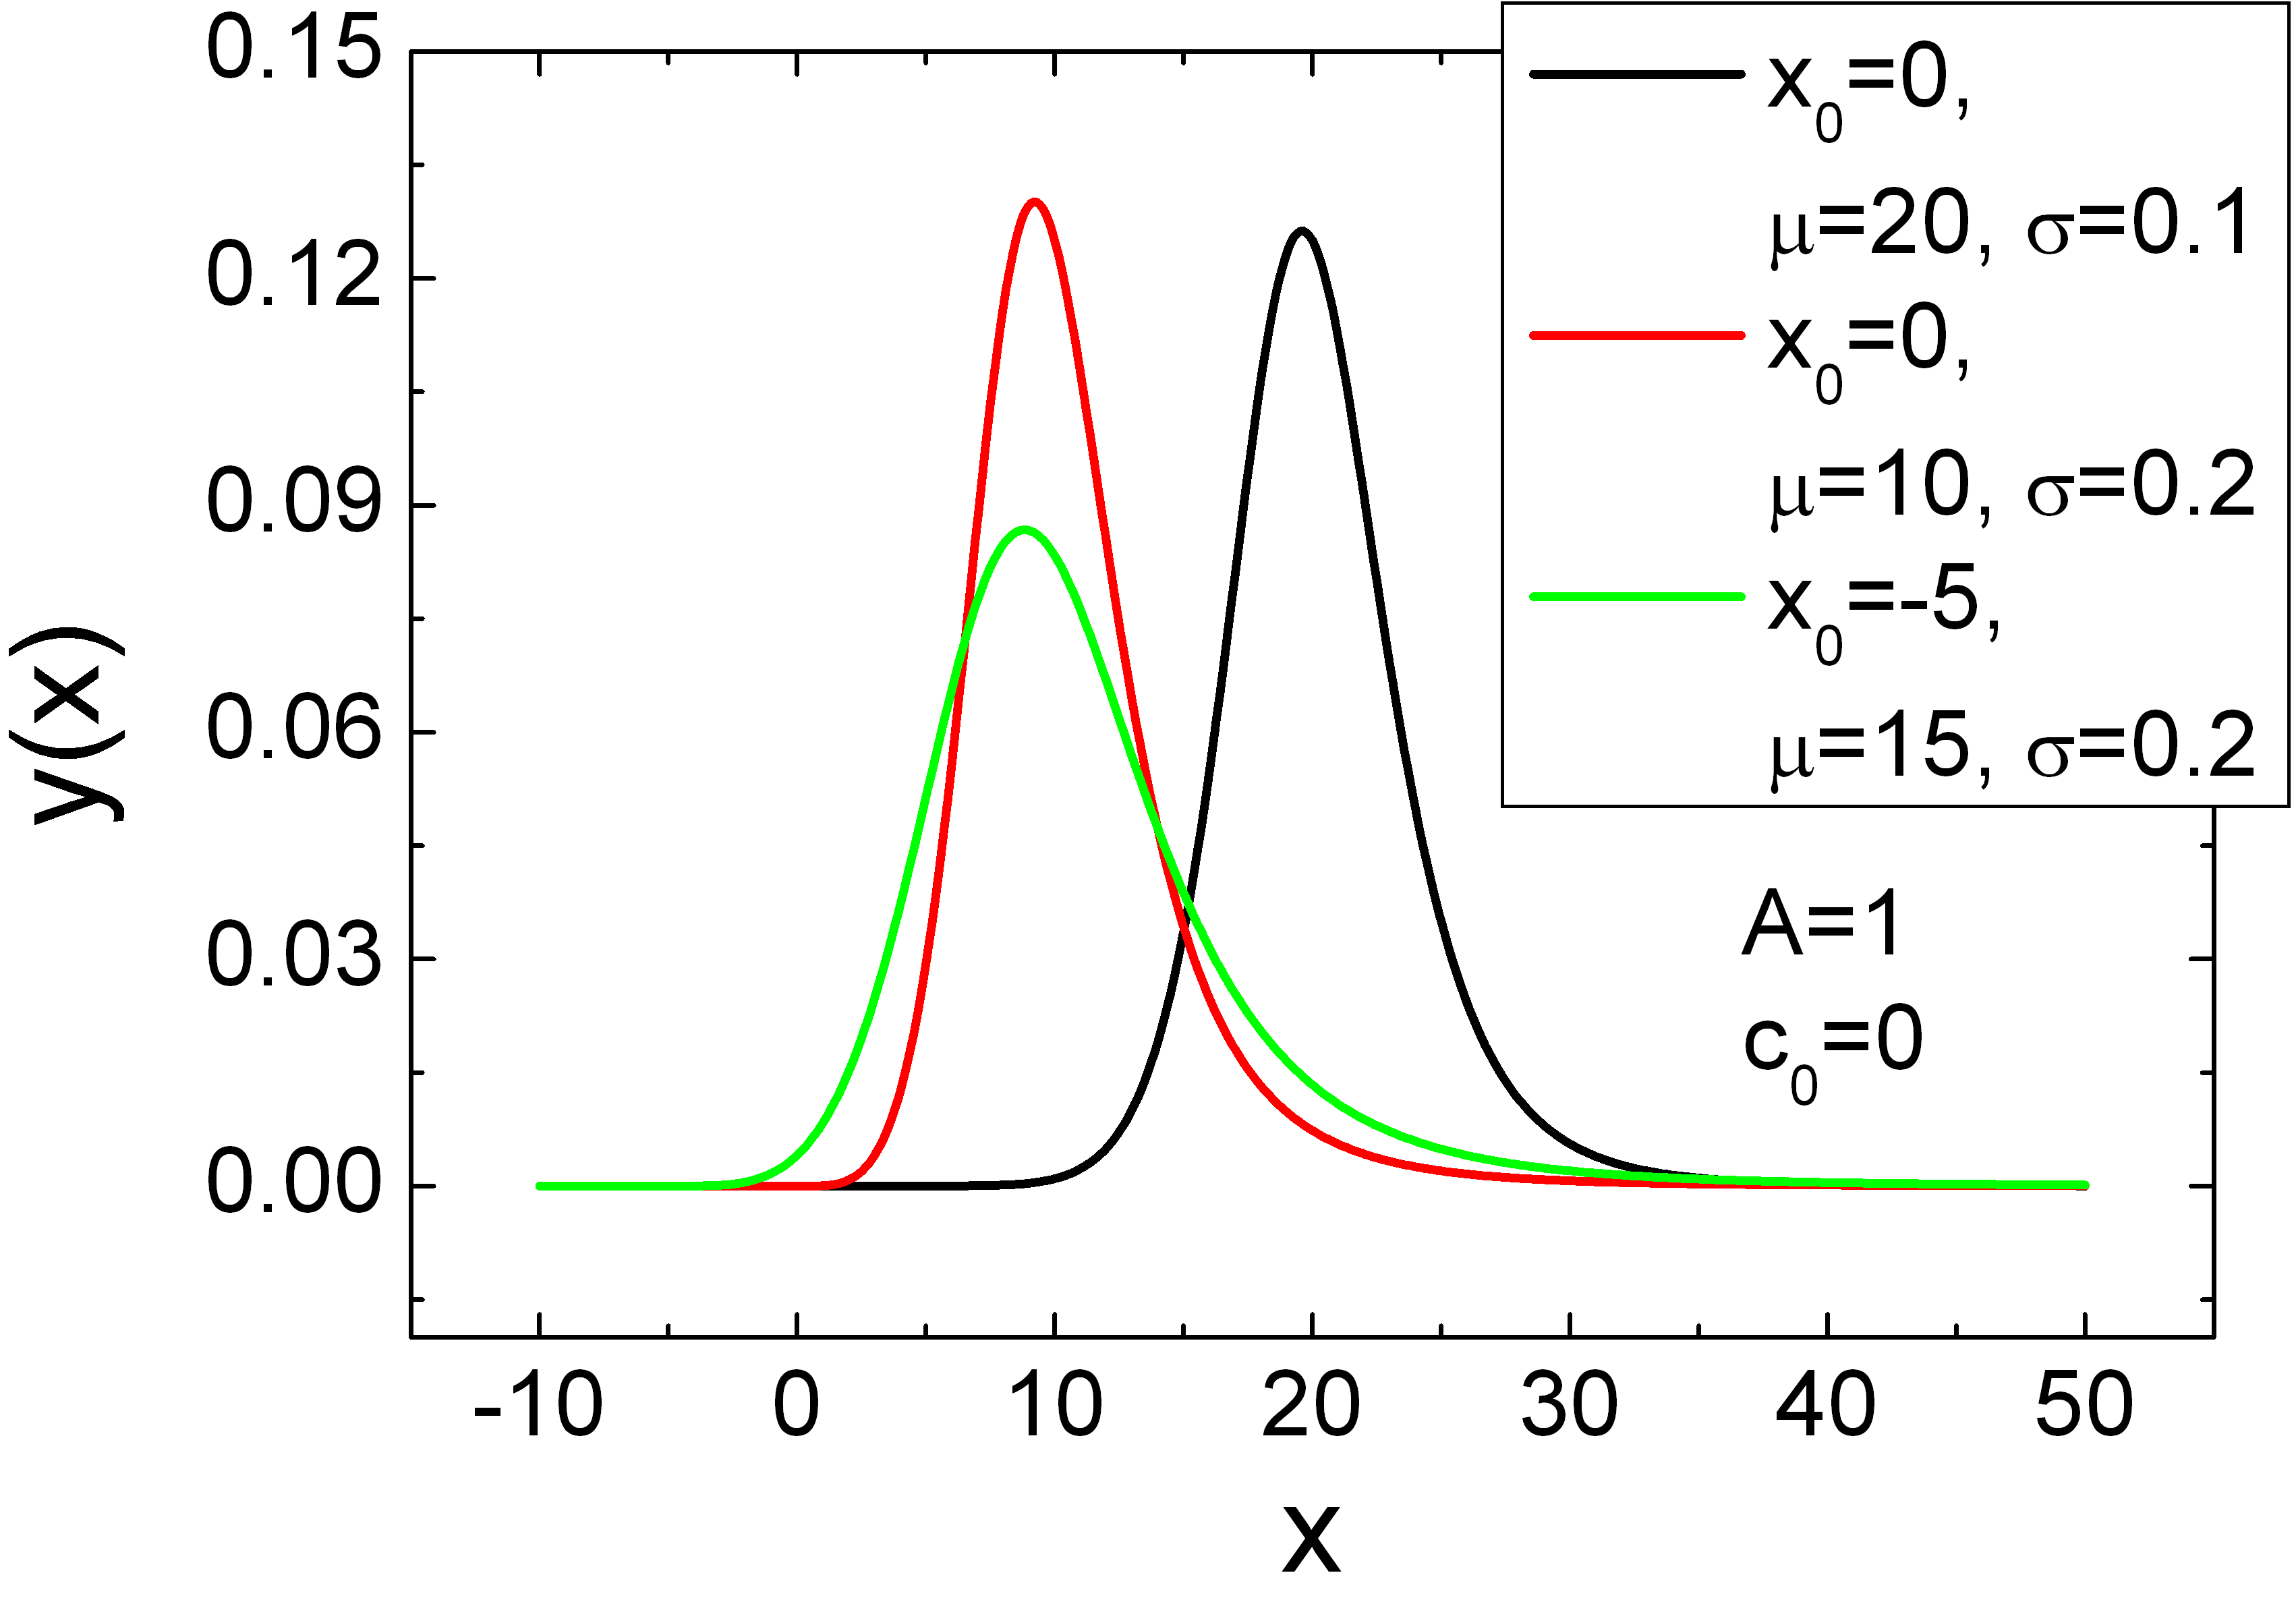
\includegraphics[width=0.6824\textwidth]{LogLogisticArea.png}
\end{center}
\caption{Plot of \texttt{LogLogistic (Area)} distribution.}
\label{fig:LogLogisticArea}
\end{figure}
%%%%%%%%%%%%%%%%%%%%%%%%%%%%%%%%%%%%%%%%%%%%%%%%%%%%%%%%%%%%%%%%%%%%%%%%%%%%%%%%
\clearpage

\section{Lognormal 4-Parameter} ~\\
\label{sec:LogNormal4Parameter}
\subsection{Lognormal 4-Parameter (Amplitude)} ~\\
\label{sec:LogNormal4ParameterAmplitude}

\begin{align}
y(x) & =
\begin{cases}
c_0+A \exp\left[ - \frac{\ln(2)\ln\left(\frac{(x-x_0)(\gamma^2-1)}{\sigma\gamma}+1\right)^2}{\ln(\gamma)}\right] & \mbox{for } \gamma \neq 1, \gamma > 0 \\
c_0+A 2^{-4\left(\frac{x-x_0}{\sigma}\right)^2} & \mbox{for } \gamma = 1
\end{cases}
\end{align}
For $\left(x \geq x_0-\frac{\sigma\gamma}{\gamma^2-1} \wedge \gamma < 1\right)
\vee \left(x \leq x_0-\frac{\sigma\gamma}{\gamma^2-1} \wedge \gamma > 1\right)$ the function returns $c_0$.
\vspace{2mm}

\underline{Required parameters:}
\begin{description}
    \item[amplitude] amplitude $A$ of the LogLogistic distribution
    \item[x0] location parameter $x_0$
    \item[sigma] width parameter $\sigma > 0$
    \item[gamma] shape parameters $\gamma > 0$
    \item[backgr] offset $c_0$
\end{description}

\underline{Note}
\begin{itemize}
  \item the width parameter needs to be larger than zero $\sigma > 0$
  \item the shape parameter needs to be larger than zero $\gamma > 0$
  \item Default (size) distribution: Monodisperse
\end{itemize}

\begin{figure}[htb]
\begin{center}
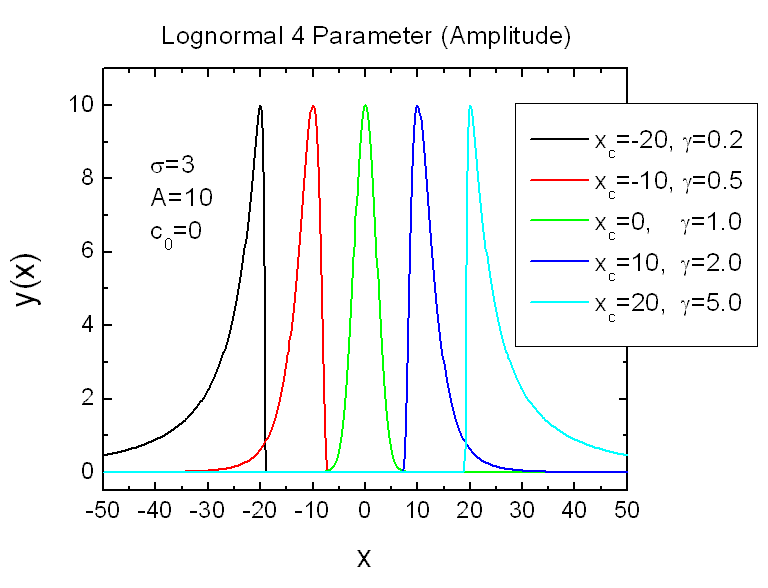
\includegraphics[width=0.6824\textwidth]{LogNormal4ParameterAmplitude.png}
\end{center}
\caption{Plot of \texttt{Lognormal 4-Parameter (Amplitude)} distribution.}
\label{fig:LogNormal4ParameterAmplitude}
\end{figure}
%%%%%%%%%%%%%%%%%%%%%%%%%%%%%%%%%%%%%%%%%%%%%%%%%%%%%%%%%%%%%%%%%%%%%%%%%%%%%%%%
\clearpage
\subsection{Lognormal 4-Parameter (Area)} ~\\
\label{sec:LogNormal4ParameterArea}

\begin{align}
y(x) & =
\begin{cases}
c_0+A \frac{\sqrt{\ln 2}(\gamma^2-1)}{\sigma\gamma\ln(\gamma)\sqrt{\pi}\exp\left(\frac{\ln(\gamma^2)}{4\ln 2}\right)}
\exp\left[ - \frac{\ln(2)\ln\left(\frac{(x-x_0)(\gamma^2-1)}{\sigma\gamma}+1\right)^2}{\ln(\gamma)}\right] & \mbox{for } \gamma \neq 1, \gamma > 0 \\
c_0+A \frac{\sqrt{\ln 2}}{\sigma\sqrt{\pi}} 2^{-4\left(\frac{x-x_0}{\sigma}\right)^2} & \mbox{for } \gamma = 1
\end{cases}
\end{align}
For $\left(x \geq x_0-\frac{\sigma\gamma}{\gamma^2-1} \wedge \gamma < 1\right)
\vee \left(x \leq x_0-\frac{\sigma\gamma}{\gamma^2-1} \wedge \gamma > 1\right)$ the function returns $c_0$.
\vspace{2mm}

\underline{Required parameters:}
\begin{description}
    \item[area] area $A$ of the LogLogistic distribution
    \item[x0] location parameter $x_0$
    \item[sigma] width parameter $\sigma > 0$
    \item[gamma] shape parameters $\gamma > 0$
    \item[backgr] offset $c_0$
\end{description}

\underline{Note}
\begin{itemize}
  \item the width parameter needs to be larger than zero $\sigma > 0$
  \item the shape parameter needs to be larger than zero $\gamma > 0$
  \item Default (size) distribution: Monodisperse
\end{itemize}


\begin{figure}[htb]
\begin{center}
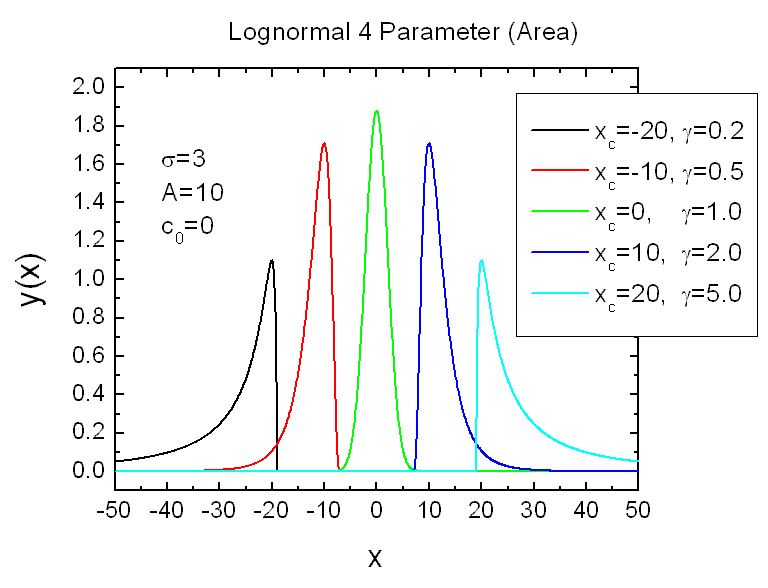
\includegraphics[width=0.6824\textwidth]{LogNormal4ParameterArea.png}
\end{center}
\caption{Plot of \texttt{Lognormal 4-Parameter (Area)} distribution.}
\label{fig:LogNormal4ParameterArea}
\end{figure}

%%%%%%%%%%%%%%%%%%%%%%%%%%%%%%%%%%%%%%%%%%%%%%%%%%%%%%%%%%%%%%%%%%%%%%%%%%%%%%%%
\clearpage
\section{LogNormal}
\label{sec:LogNormal}
The LogNormal distribution is defined with reference to the normal
distribution. A random variable is Lognormally distributed if the
logarithm of the random variable is normally distributed.

The LogNormal distribution is commonly used for general reliability
analysis, cycles-to-failure in fatigue, material strengths and
loading variables in probabilistic design. Another advantage of the
LogNormal distribution is that it is positive-definite, so it is
often useful for representing quantities that cannot have negative
values. LogNormal distributions have proven useful as distributions
for rainfall amounts, for the size distributions of aerosol
particles or droplets, and for many other cases. The log-normal
distribution has the probability density function
\begin{equation}
f(x') = \frac{1}{\sigma\sqrt{2\pi}} \exp\left(-\frac{1}{2}\left(\frac{x'-\mu'}{\sigma}\right)^2\right)
\end{equation}
where $\mu'= \ln(\mu)$ and  $x'= \ln(x)$.
The lognormal pdf can be obtained, realizing that for equal probabilities
under the normal and lognormal pdfs, incremental areas should also be equal, or:
\begin{equation}%\label{}
    f(x;\mu,\sigma)dx =f(x';\mu,\sigma)dx'
\end{equation}
Taking the derivative yields:
\begin{equation}%\label{}
    dx' =\frac{dx}{x}
\end{equation}
Substitution yields:
\begin{equation}%\label{}
    f(x;\mu,\sigma) =\frac{f(x';\mu,\sigma)}{x}
\end{equation}
where:
\begin{equation}
    f(x;\mu,\sigma) =
        \frac{1}{x\sigma \sqrt{2 \pi}}\exp\left(-\frac{1}{2}\left(\frac{\ln (x) -
        \ln(\mu)}{\sigma}\right)^2\right)
\end{equation}
for $x\in (0,\infty]$, where  $\mu>0$ and $\sigma\neq 0$ are the location and scale
parameter. The mode of the distribution is
\begin{equation}
\mathrm{mode} =   \mu\exp\left(-\sigma^2\right)
\end{equation}

\clearpage

\subsection{LogNormal (Amplitude)} ~\\
\label{sec:LogNormalAmplitude}
\begin{align}
y(x) &=
\begin{cases}
        \frac{A \exp\left(-\frac12\sigma^2\right) \mu}{x-x_0}\exp\left(-\frac{1}{2}\left(\frac{\ln (x-x_0) -
        \ln(\mu)}{\sigma}\right)^2\right) + c_0 & \mbox{for } x>x_0 \\
        c_0 & \mbox{for } x \leq x_0
\end{cases}
\end{align}

\underline{Required parameters:}
\begin{description}
    \item[amplitude] amplitude $A$ of the LogNormal distribution
    \item[mu] location parameter $\mu$
    \item[sigma] width parameter $\sigma > 0$
    \item[x0] shift parameters $x_0$
    \item[backgr] offset $c_0$
\end{description}

\underline{Note}
\begin{itemize}
  \item the width parameter needs to be larger than zero $\sigma > 0$
  \item the location parameter needs to be larger than the shift parameter $\mu > x_0$
  \item Default (size) distribution: Monodisperse
\end{itemize}

\begin{figure}[htb]
\begin{center}
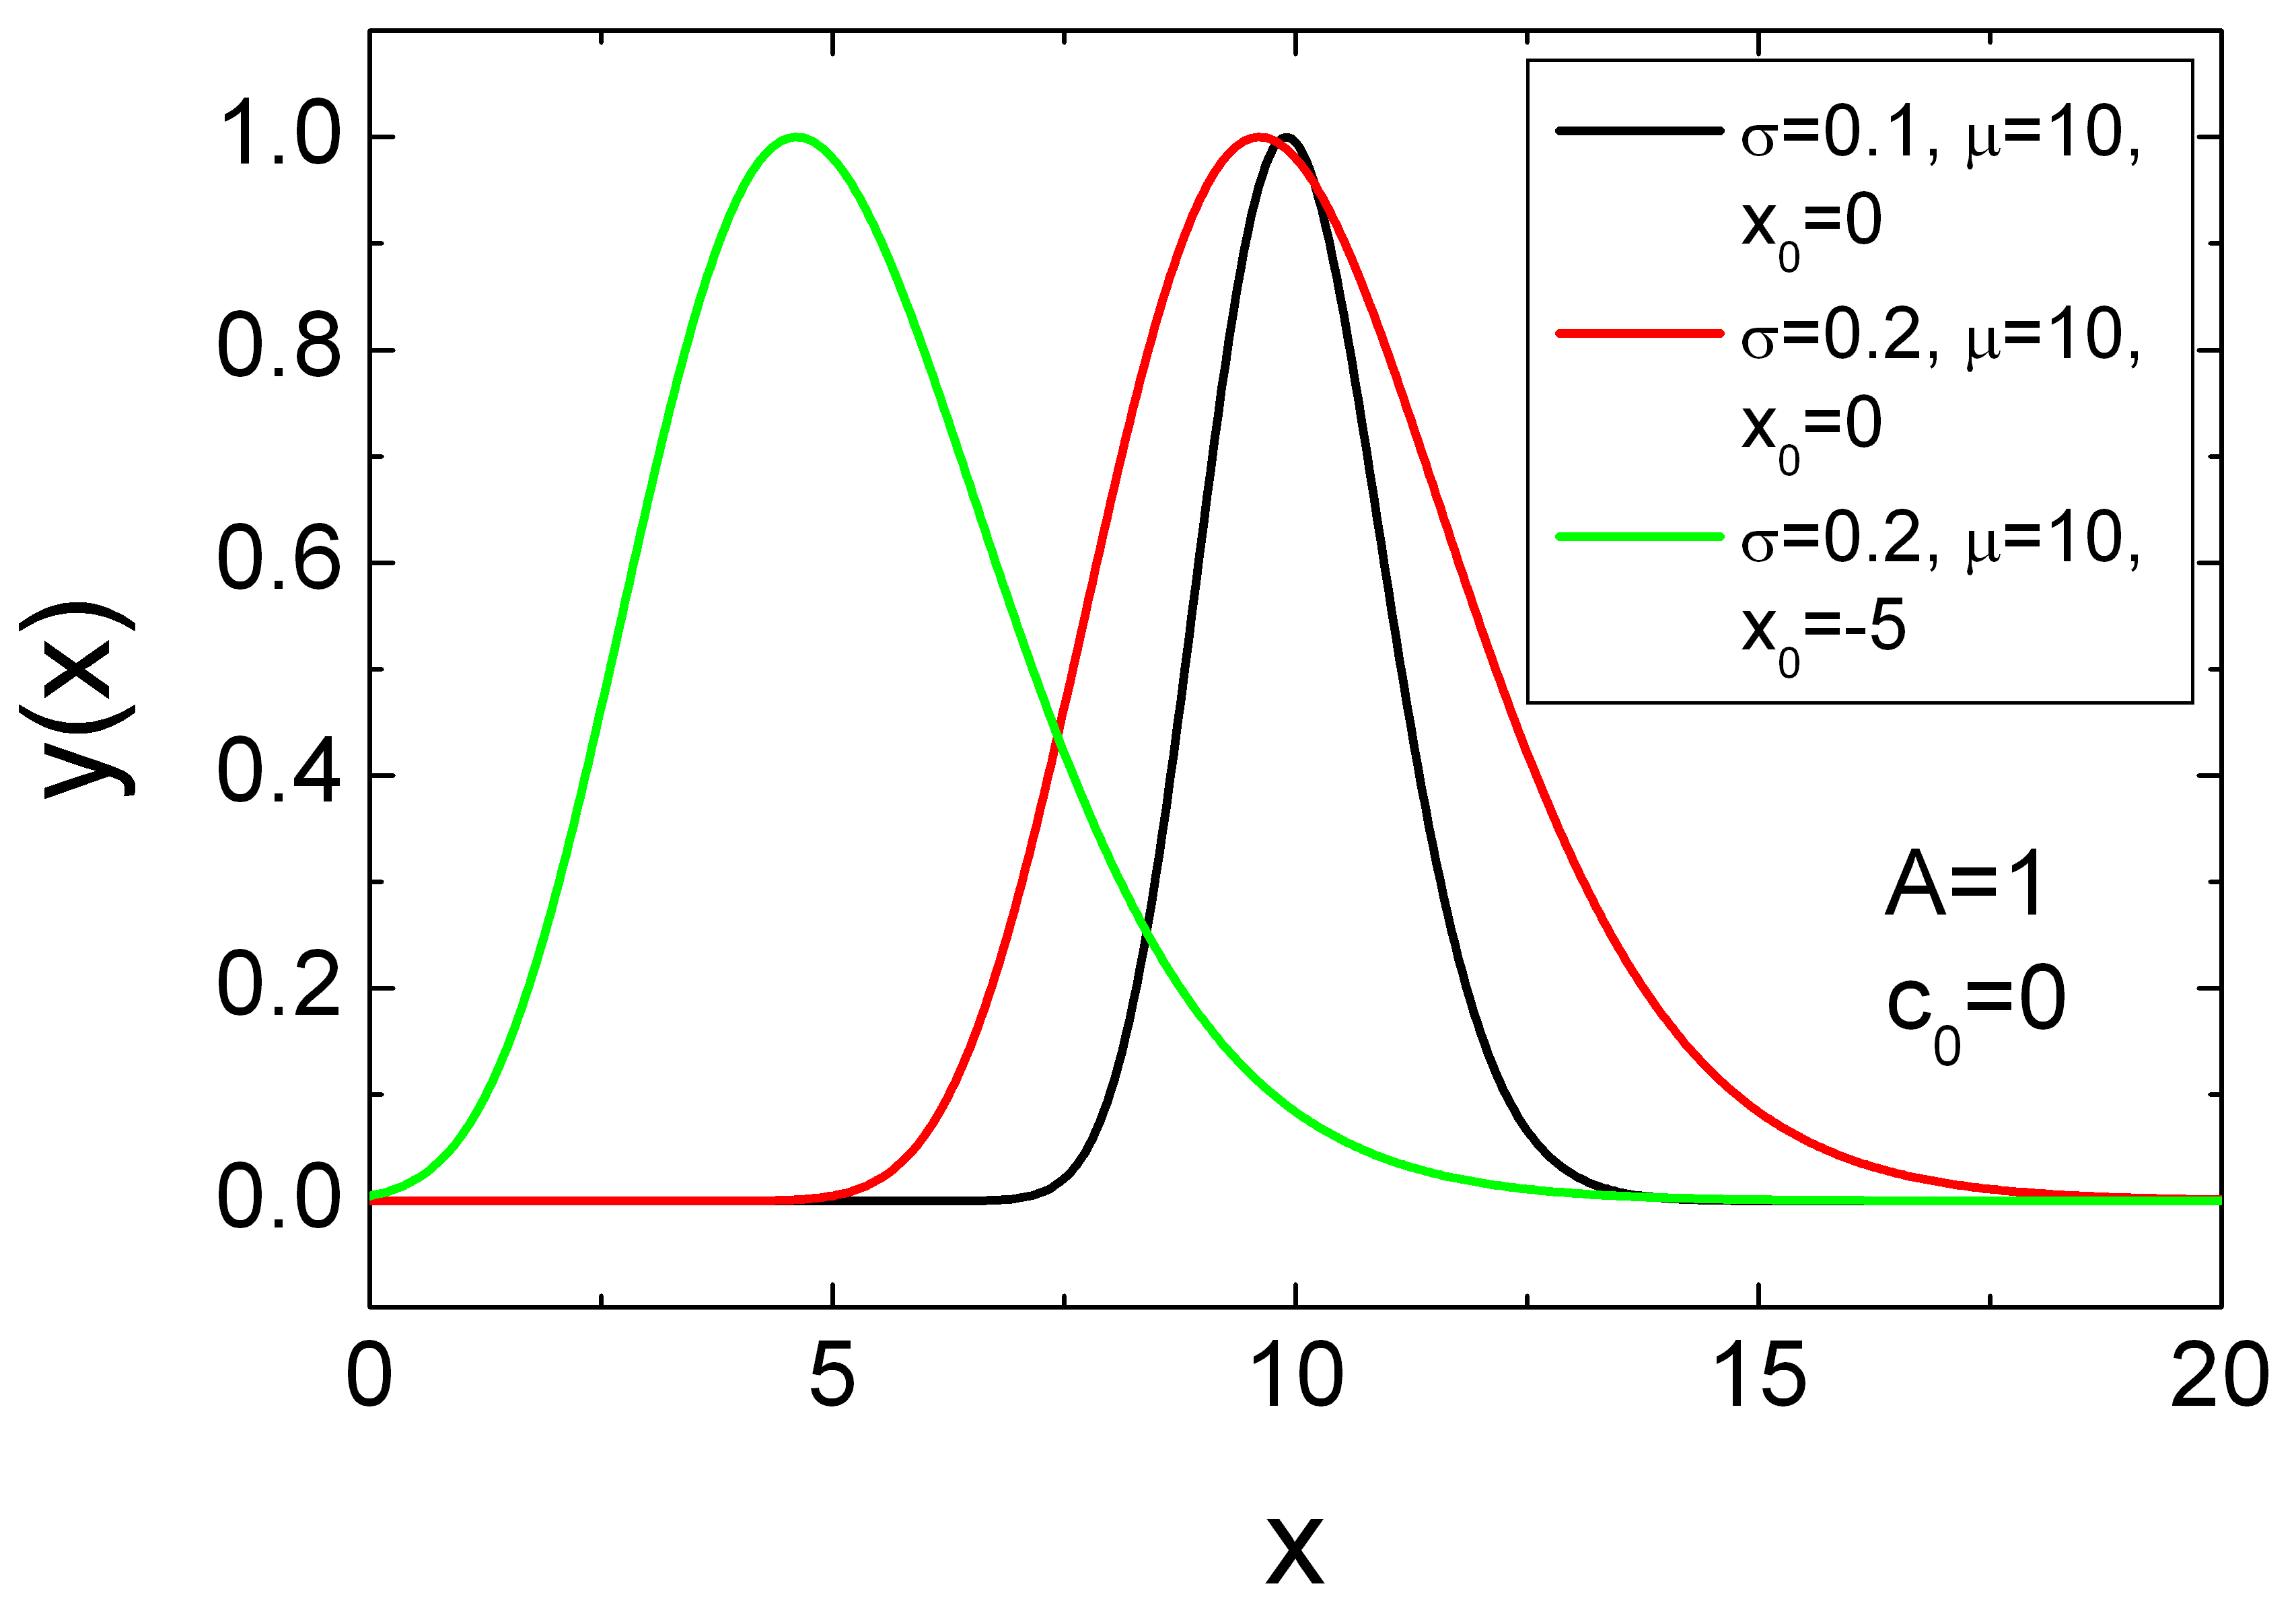
\includegraphics[width=0.6824\textwidth]{LogNormalAmplitude.png}
\end{center}
\caption{Plot of \texttt{LogNormal (Amplitude)} distribution.}
\label{fig:LogNormalAmplitude}
\end{figure}

\clearpage
\subsection{LogNormal (Area)} ~\\
\label{sec:LogNormalArea}
\begin{align}
y(x) &=
\begin{cases}
        \frac{A}{(x-x_0)\sigma \sqrt{2 \pi}}
        \exp\left(-\frac{1}{2}\left(\frac{\ln (x-x_0) -
        \ln(\mu)}{\sigma}\right)^2\right) + c0 & \mbox{for } x>x0 \\
        c_0 & \mbox{for } x \leq x0
\end{cases}
\end{align}

\underline{Required parameters:}
\begin{description}
    \item[area] area $A$ of the LogNormal distribution
    \item[mu] location parameter $\mu$
    \item[sigma] width parameter $\sigma > 0$
    \item[x0] shift parameters $x_0$
    \item[backgr] offset $c_0$
\end{description}

\underline{Note}
\begin{itemize}
  \item the width parameter needs to be larger than zero $\sigma > 0$
  \item the location parameter needs to be larger than the shift parameter $\mu > x_0$
  \item Default (size) distribution: Monodisperse
\end{itemize}

\begin{figure}[htb]
\begin{center}
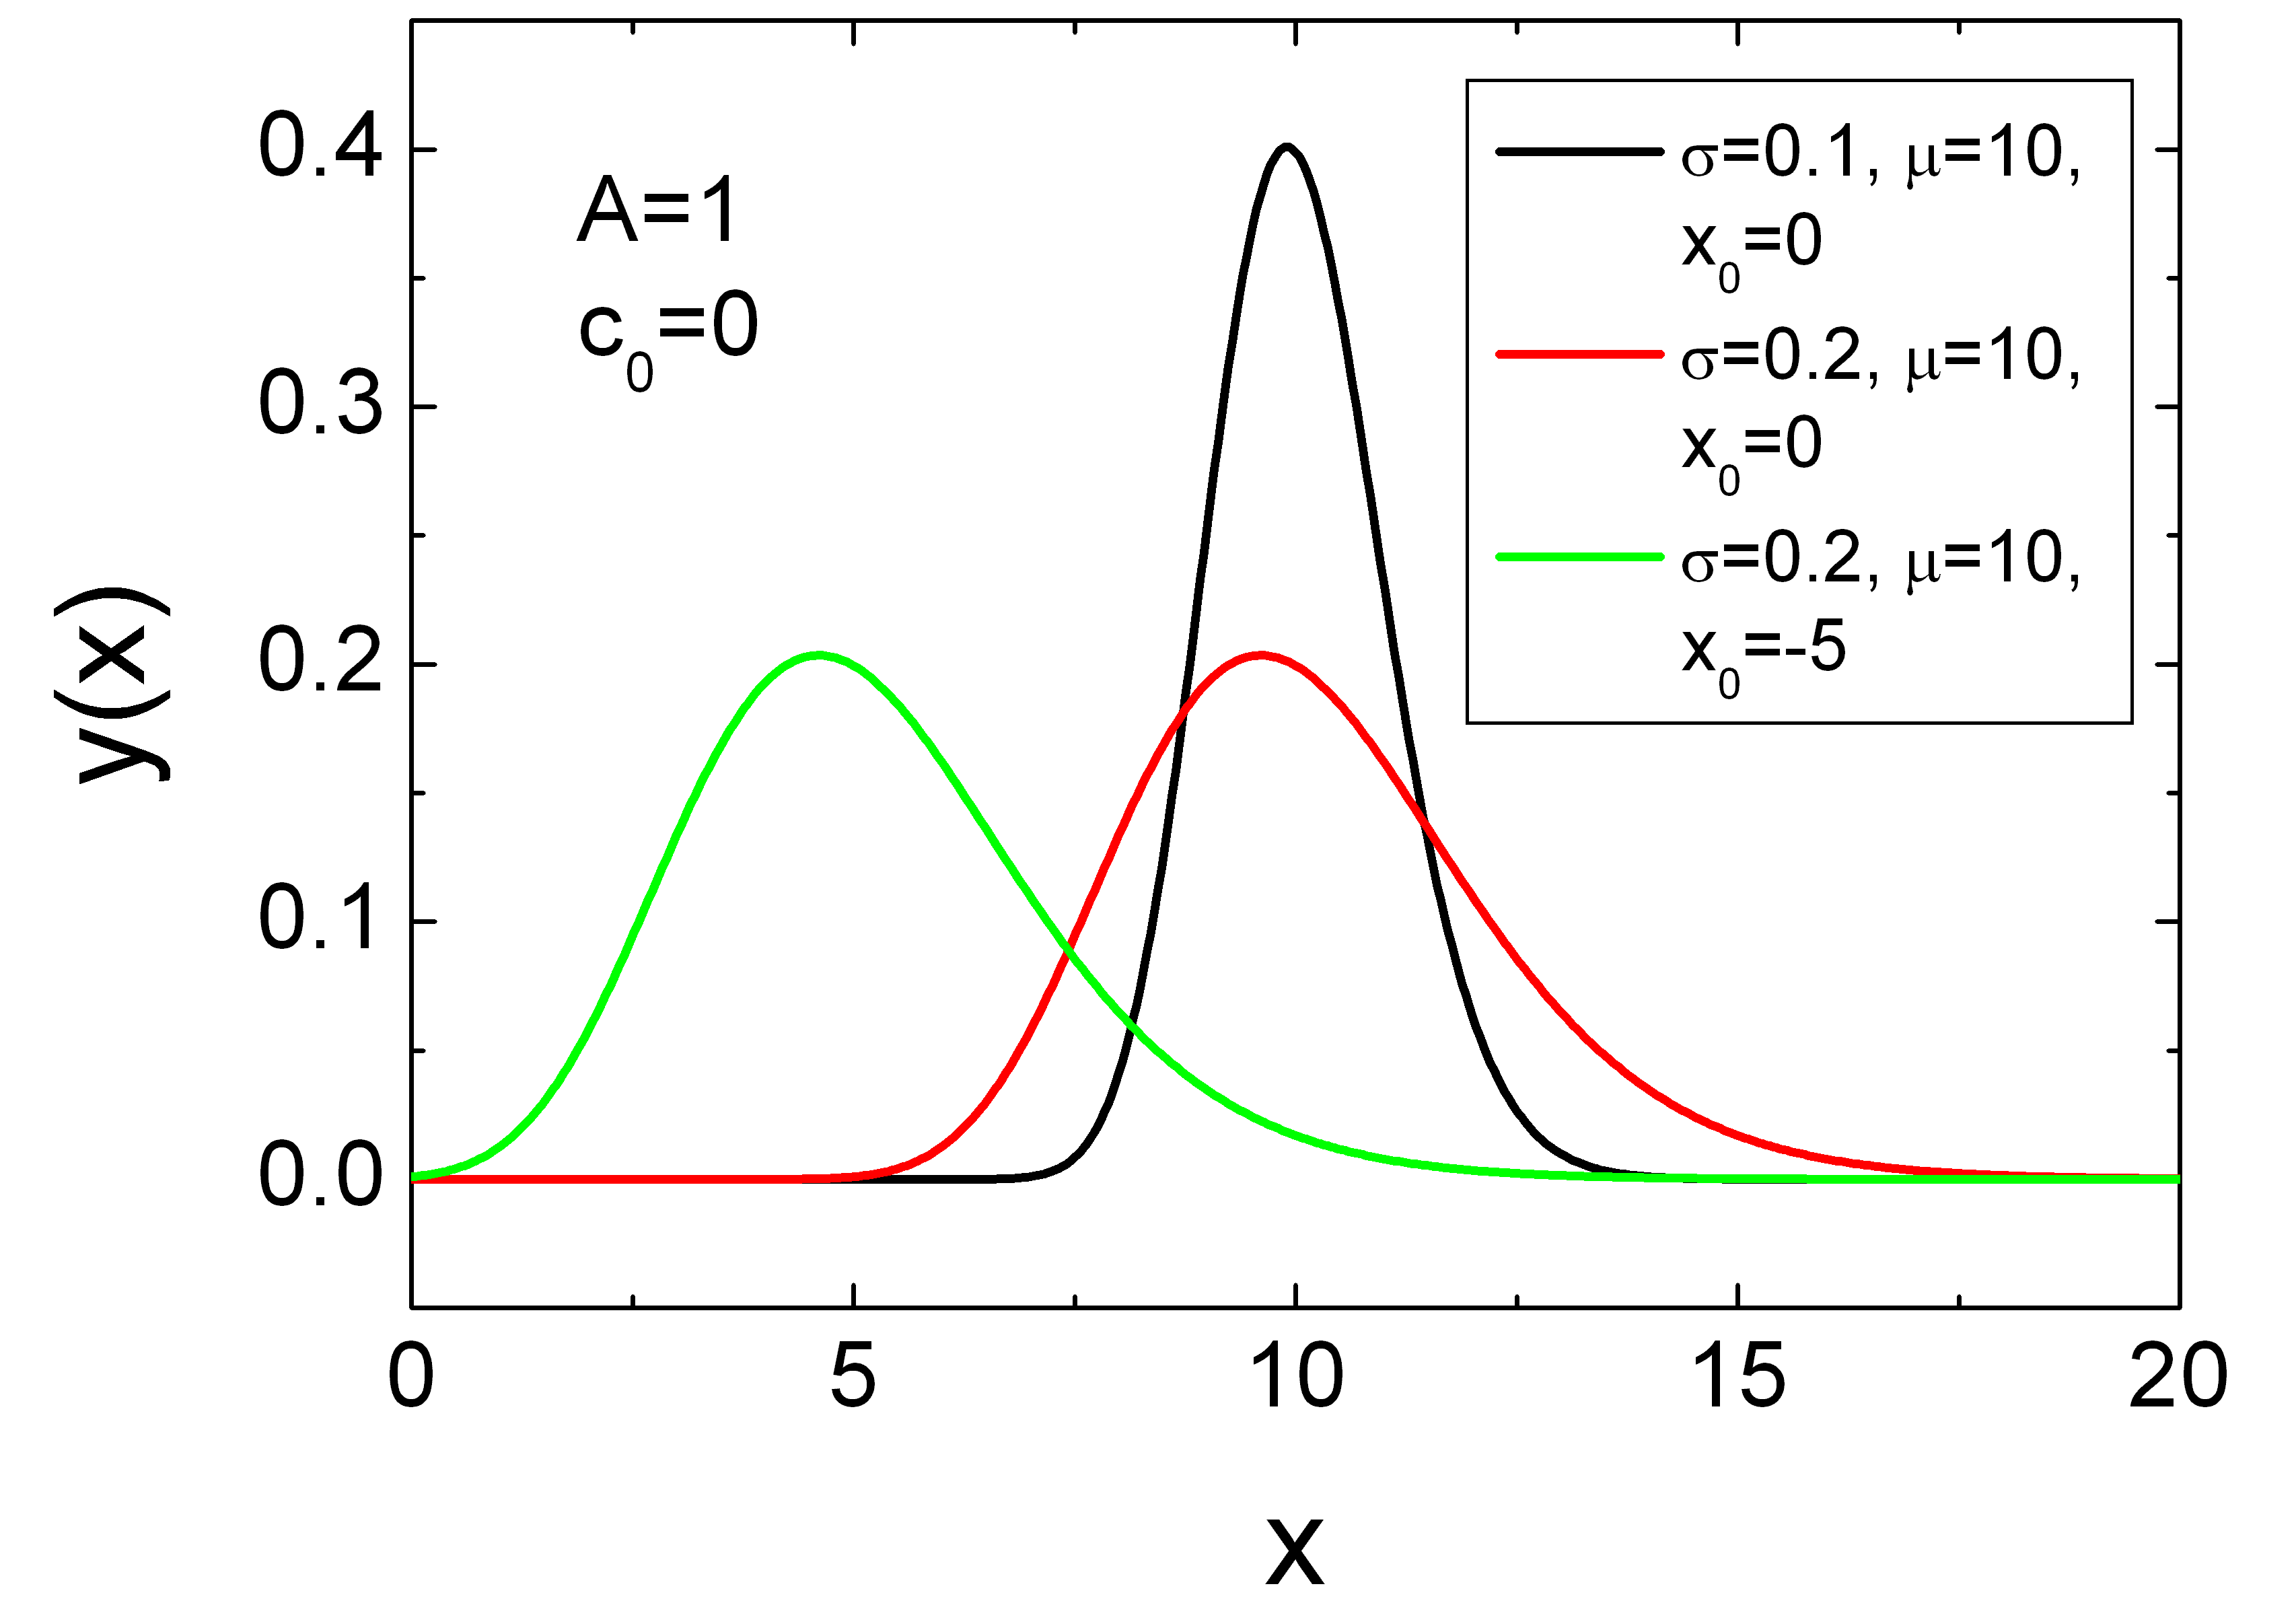
\includegraphics[width=0.6824\textwidth]{LogNormalArea.png}
\end{center}
\caption{Plot of \texttt{LogNormal (Area)} distribution.}
\label{fig:LogNormalArea}
\end{figure}

%%%%%%%%%%%%%%%%%%%%%%%%%%%%%%%%%%%%%%%%%%%%%%%%%%%%%%%%%%%%%%%%%%%%%%%%%%%%%%%%
\clearpage
\section{Lorentzian or Cauchy distribution}
\label{sec:Lorentzian}

The Cauchy�Lorentz Distribution, named after
Augustin Cauchy and Hendrik Lorentz, is a continuous probability
distribution. As a probability distribution, it is known as the
Cauchy distribution, while among physicists, it is known as a
Lorentz distribution, or a Lorentz(ian) function or the Breit�Wigner
distribution. Its importance in physics is due to it being the solution to the
differential equation describing forced resonance. The Lorntzian
distribution has the probability density function
\begin{align}
 f(x; x_0,\sigma)&= \frac{1}{\pi\sigma \left[1 + \left(\frac{x-x_0}{\sigma}\right)^2\right]} \nonumber \\
                 &= { 1 \over \pi } \left[ { \sigma \over (x - x_0)^2 + \sigma^2 } \right]
\end{align}
where $x_0$ is the location parameter, specifying the location of the
peak of the distribution, and $\sigma$ is the scale parameter which
specifies the half-width at half-maximum (HWHM).

\vspace{5mm}

\subsection{Lorentzian (Amplitude)} ~\\
\label{sec:LorentzianAmplitude}
\begin{figure}[htb]
\begin{center}
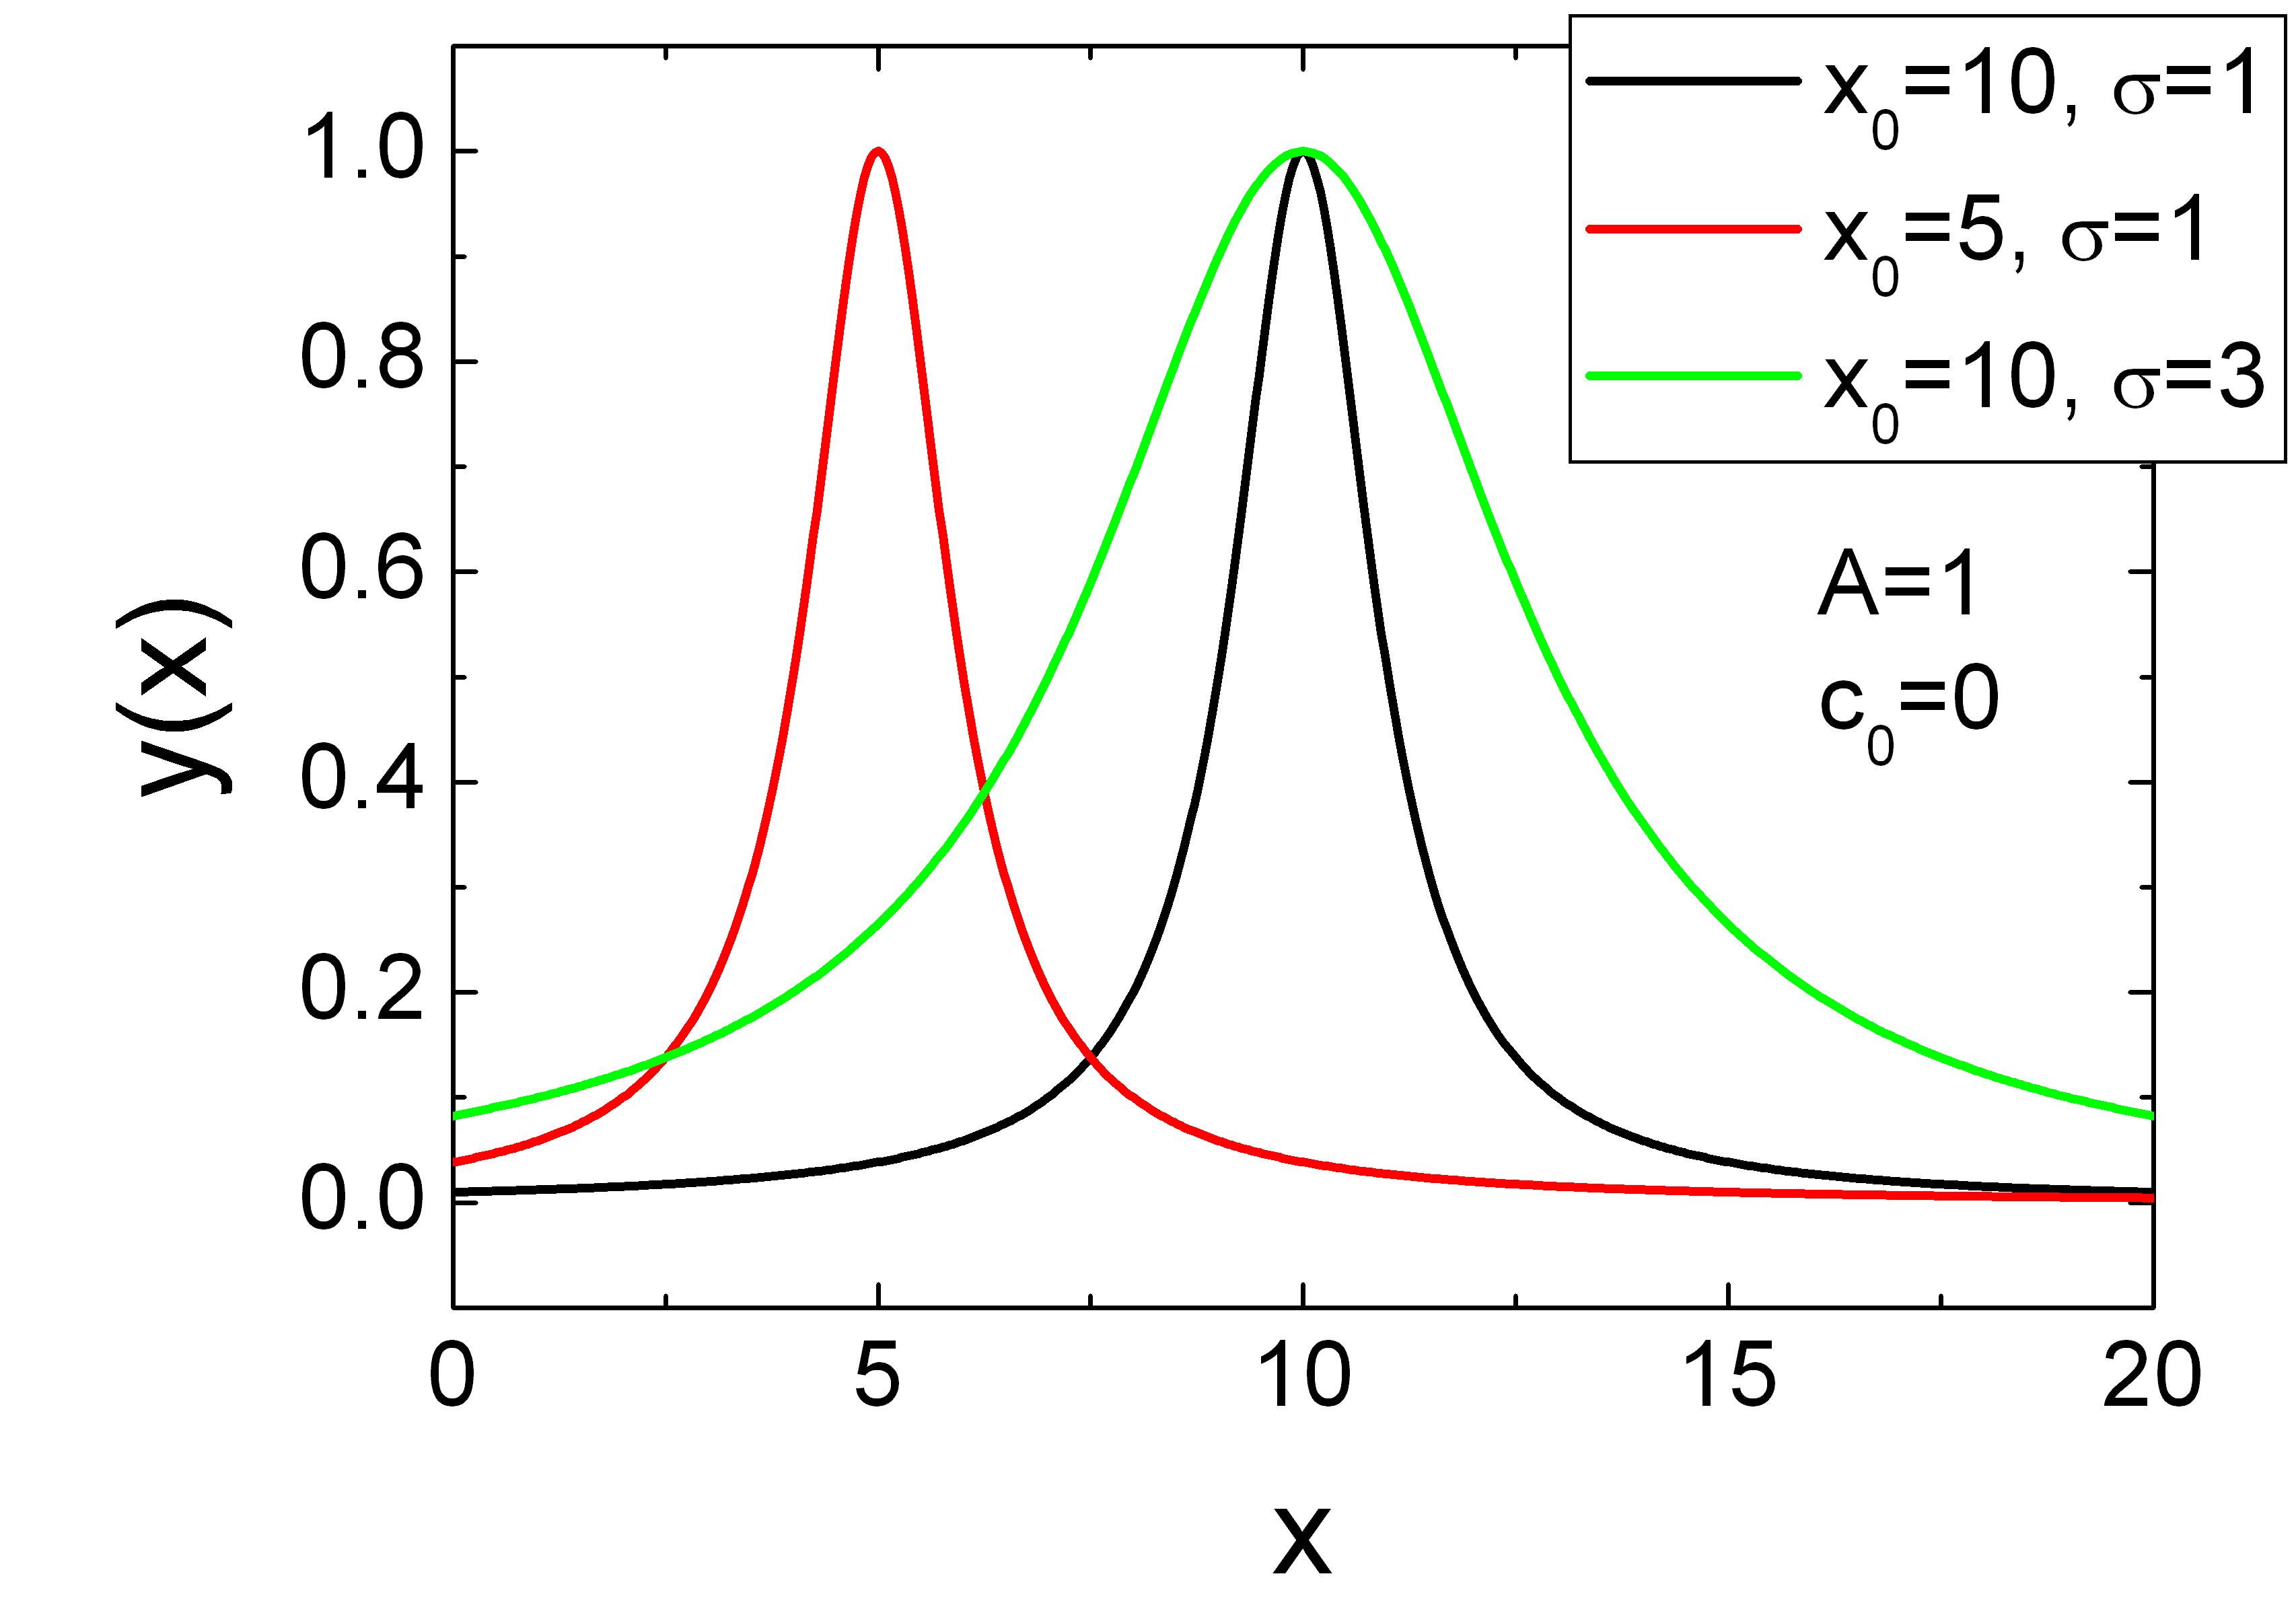
\includegraphics[width=0.6824\textwidth]{LorentzianAmplitude.png}
\end{center}
\caption{Plot of \texttt{Lorentzian (Amplitude)} distribution.}
\label{fig:LorentzianAmplitude}
\end{figure}
%%%%%%%%%%%%%%%%%%%%%%%%%%%%%%%%%%%%%%%%%%%%%%%%%%%%%%%%%%%%%%%%%%%%%%%%%%%%%%%%
\clearpage
\subsection{Lorentzian (Area)} ~\\
\label{sec:LorentzianArea}

\begin{figure}[htb]
\begin{center}
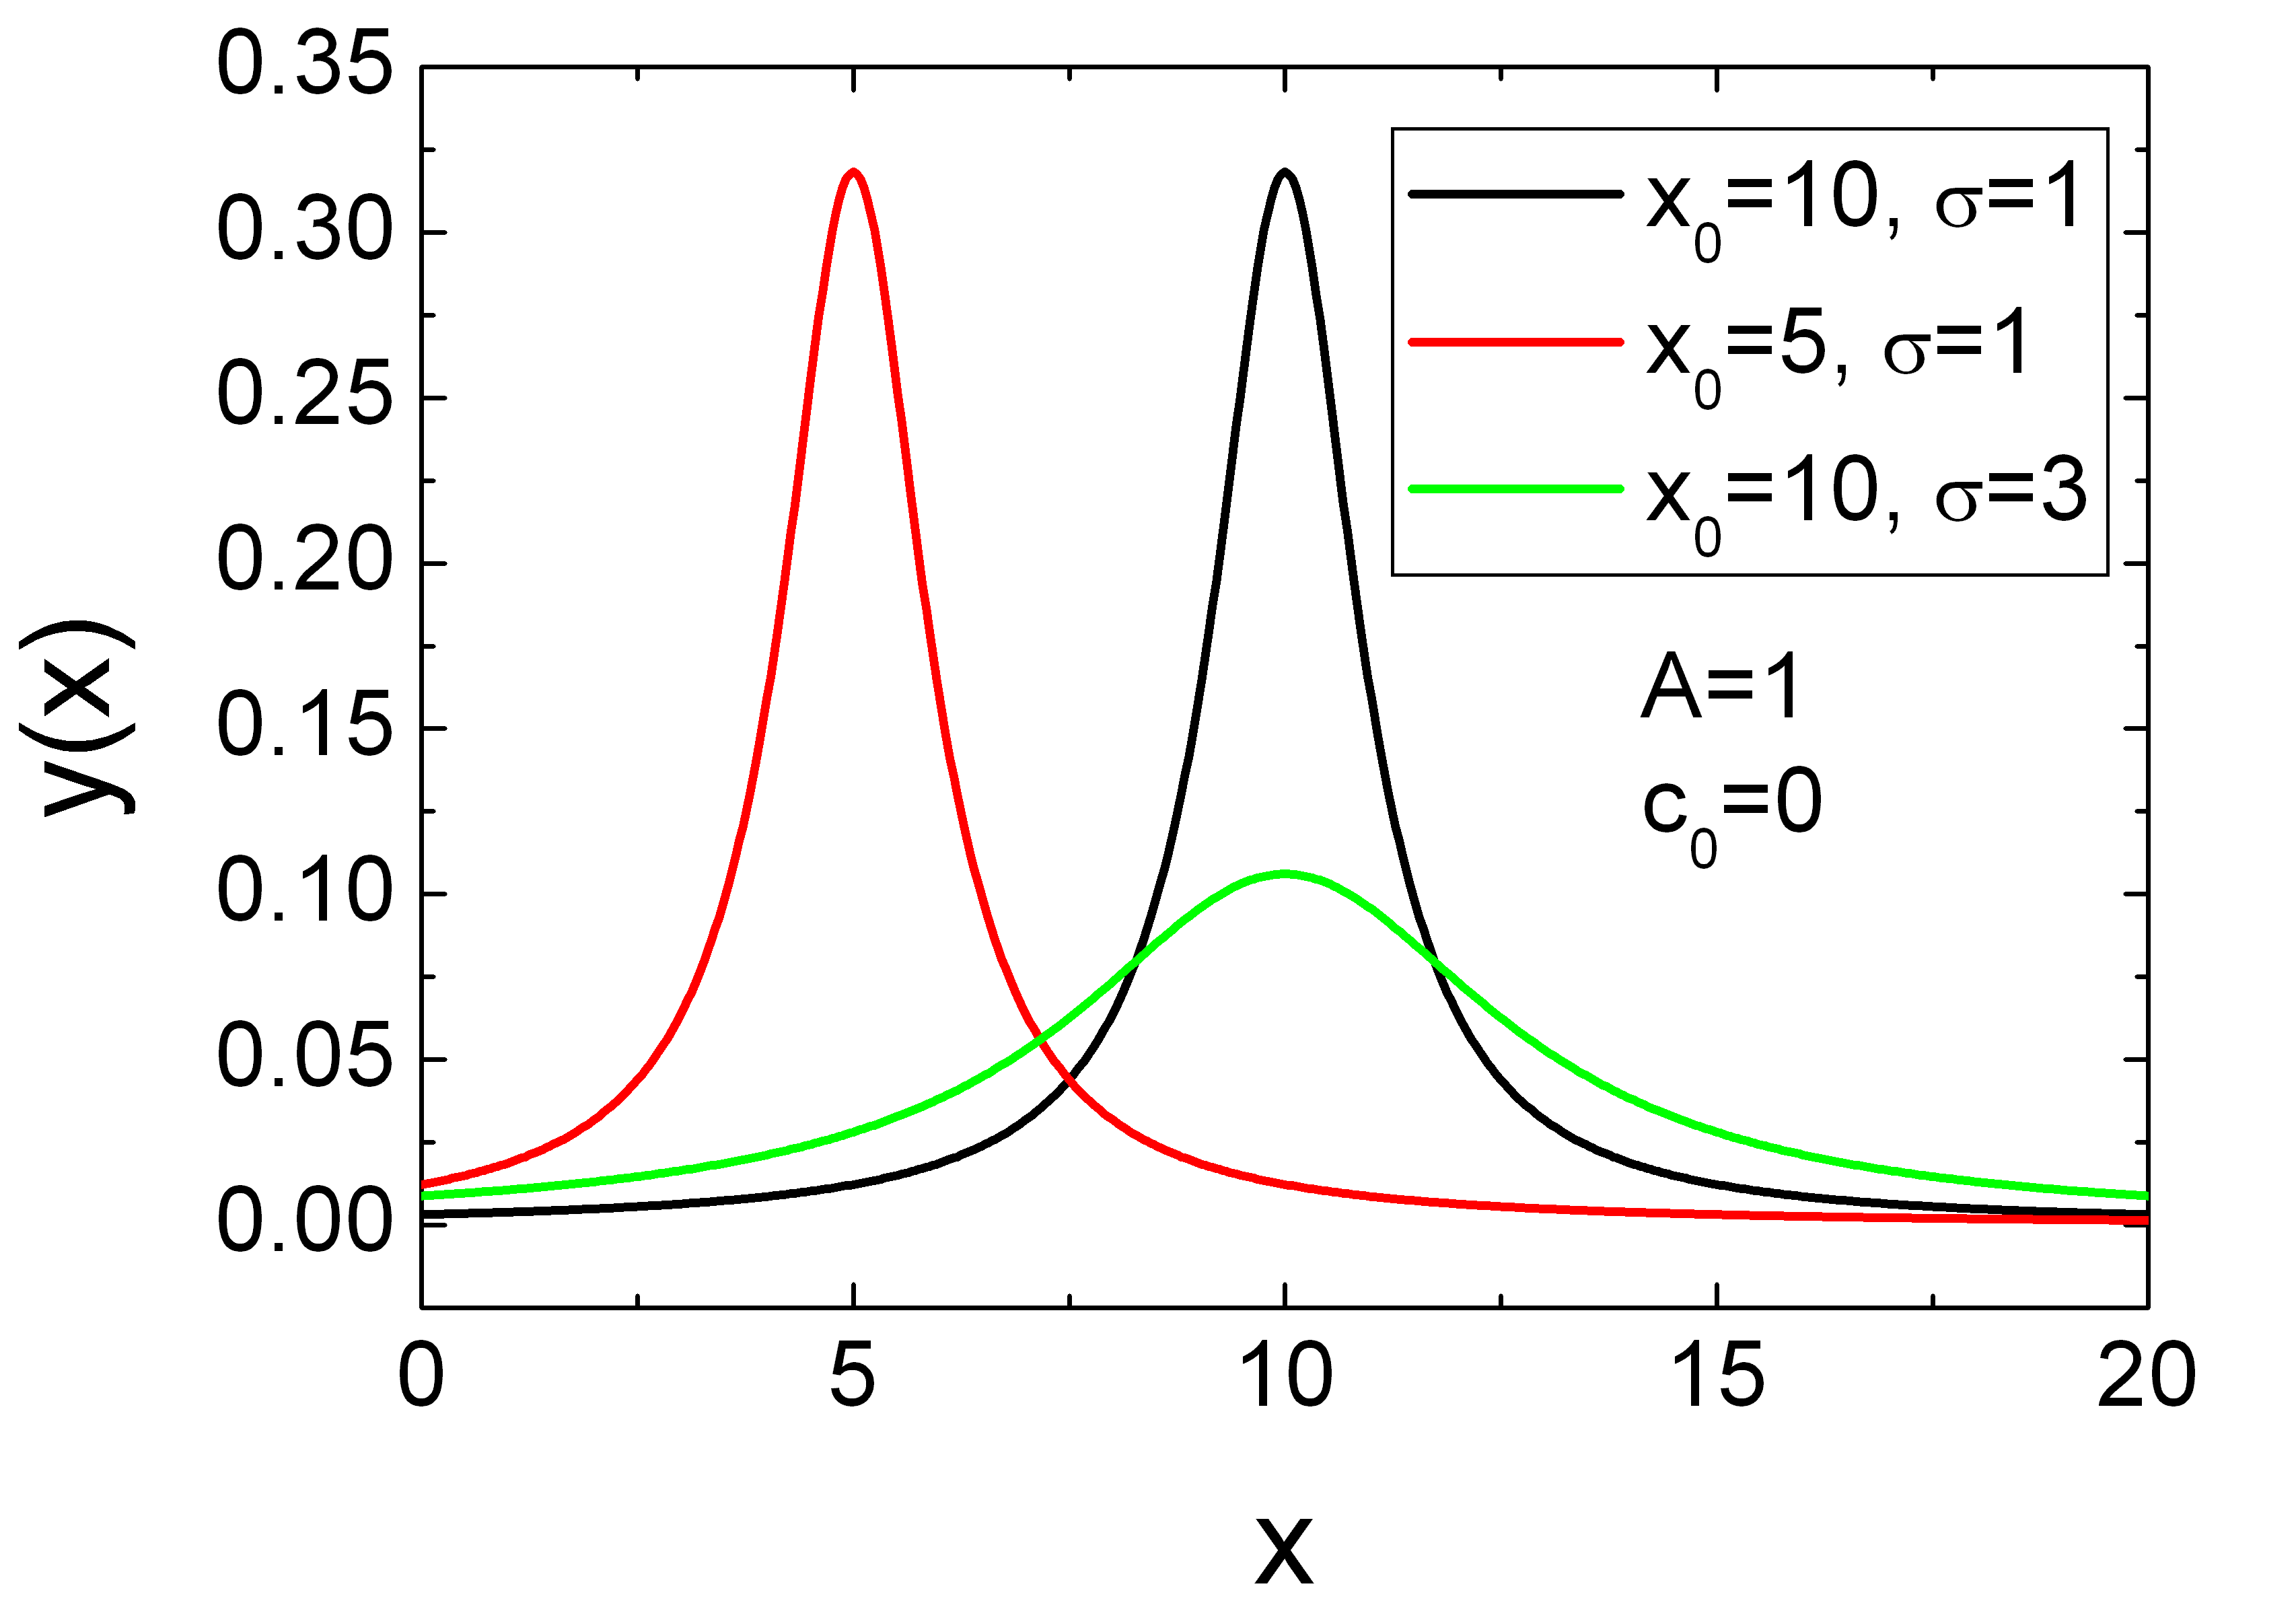
\includegraphics[width=0.6824\textwidth]{LorentzianArea.png}
\end{center}
\caption{Plot of \texttt{Lorentzian (Area)} distribution.}
\label{fig:LorentzianArea}
\end{figure}





%%%%%%%%%%%%%%%%%%%%%%%%%%%%%%%%%%%%%%%%%%%%%%%%%%%%%%%%%%%%%%%%%%%%%%%%%%%%%%%%
\clearpage
\section{Maxwell-Boltzmann distribution}
\label{sec:MaxwellBoltzmann}

The Maxwell-Boltzmann distribution describes particle speeds in
gases, where the particles do not constantly interact with each
other but move freely between short collisions. It describes the
probability of a particle's speed (the magnitude of its velocity
vector) being near a given value as a function of the temperature
of the system, the mass of the particle, and that speed value.
This probability distribution is named after James Clerk Maxwell
and Ludwig Boltzmann.

The Maxwell-Boltzmann distribution is usually thought of as the
distribution for molecular speeds, but it can also refer to the
distribution for velocities, momenta, and magnitude of the momenta
of the molecules, each of which will have a different probability
distribution function, all of which are related. Two Maxwell
distributions have been implemented, one distribution for speed
and a generalized Maxwell distribution, which includes also the
energy distribution.

The generalized Maxwell distribution is here defined as
\begin{align}
p(x; x_0, \sigma, n, m) &=
\begin{cases}
0 & \mbox{for~} x<x_0 \\
   \frac{\left(x-x_0\right)^m \exp\left(-\frac{1}{2}\left(\frac{x-x_0}{\abs{\sigma}}\right)^n\right)}{
   2^{(1+m)/n}\abs{\sigma}^{1+m} \frac{1}{\abs{n}}\Gamma\left(\frac{1+m}{n}\right)}
   & \mbox{for~} x \geq x_0 .\\
\end{cases}
\end{align}
where $x_0$ is the location parameter, specifying the location of
the peak of the distribution, and $\sigma$ is the scale parameter
which specifies the width. The mode of the distribution is given
by
\begin{align}
x_\text{mode} &= \left(\frac{2m}{n}\right)^{1/n} \abs{\sigma}+x_0
.
\end{align}
For the case $m=n=2$ one gets the "Maxwell-Boltzmann distribution"
to refers to the distribution of speed. To get the distribution
for the energy one has to set $m=1/2$ and $n=1$. In case of the
width parameter $\sigma$ always the modulus is used in the
calculation of the distribution function to avoid negative values
for which the function is not always well defined. For $\sigma=0$
the distribution function is not defined.

\clearpage
\subsection{Maxwell (Amplitude)} ~\\
\label{sec:MaxwellAmplitude}
\begin{align}
y(x;A,\sigma,x_0,y_0) &=
\begin{cases}
y_0 & \mbox{for~} x < x_0 \\
y_0 +  A \;
\frac{\left(x-x_0\right)^2}{\left(x_\text{mode}-x_0\right)^2}
        \frac{\exp\left(-\frac{1}{2}\left(\frac{x-x_0}{\sigma}\right)^2\right)}{
        \exp\left(-\frac{1}{2}\left(\frac{x_\text{mode}-x_0}{\sigma}\right)^2\right)}
& \mbox{for~} x \geq x_0
\end{cases}
\end{align}
with $x_\text{mode}=\sqrt{2}\abs{\sigma}+x_0$.

\begin{figure}[htb]
\begin{center}
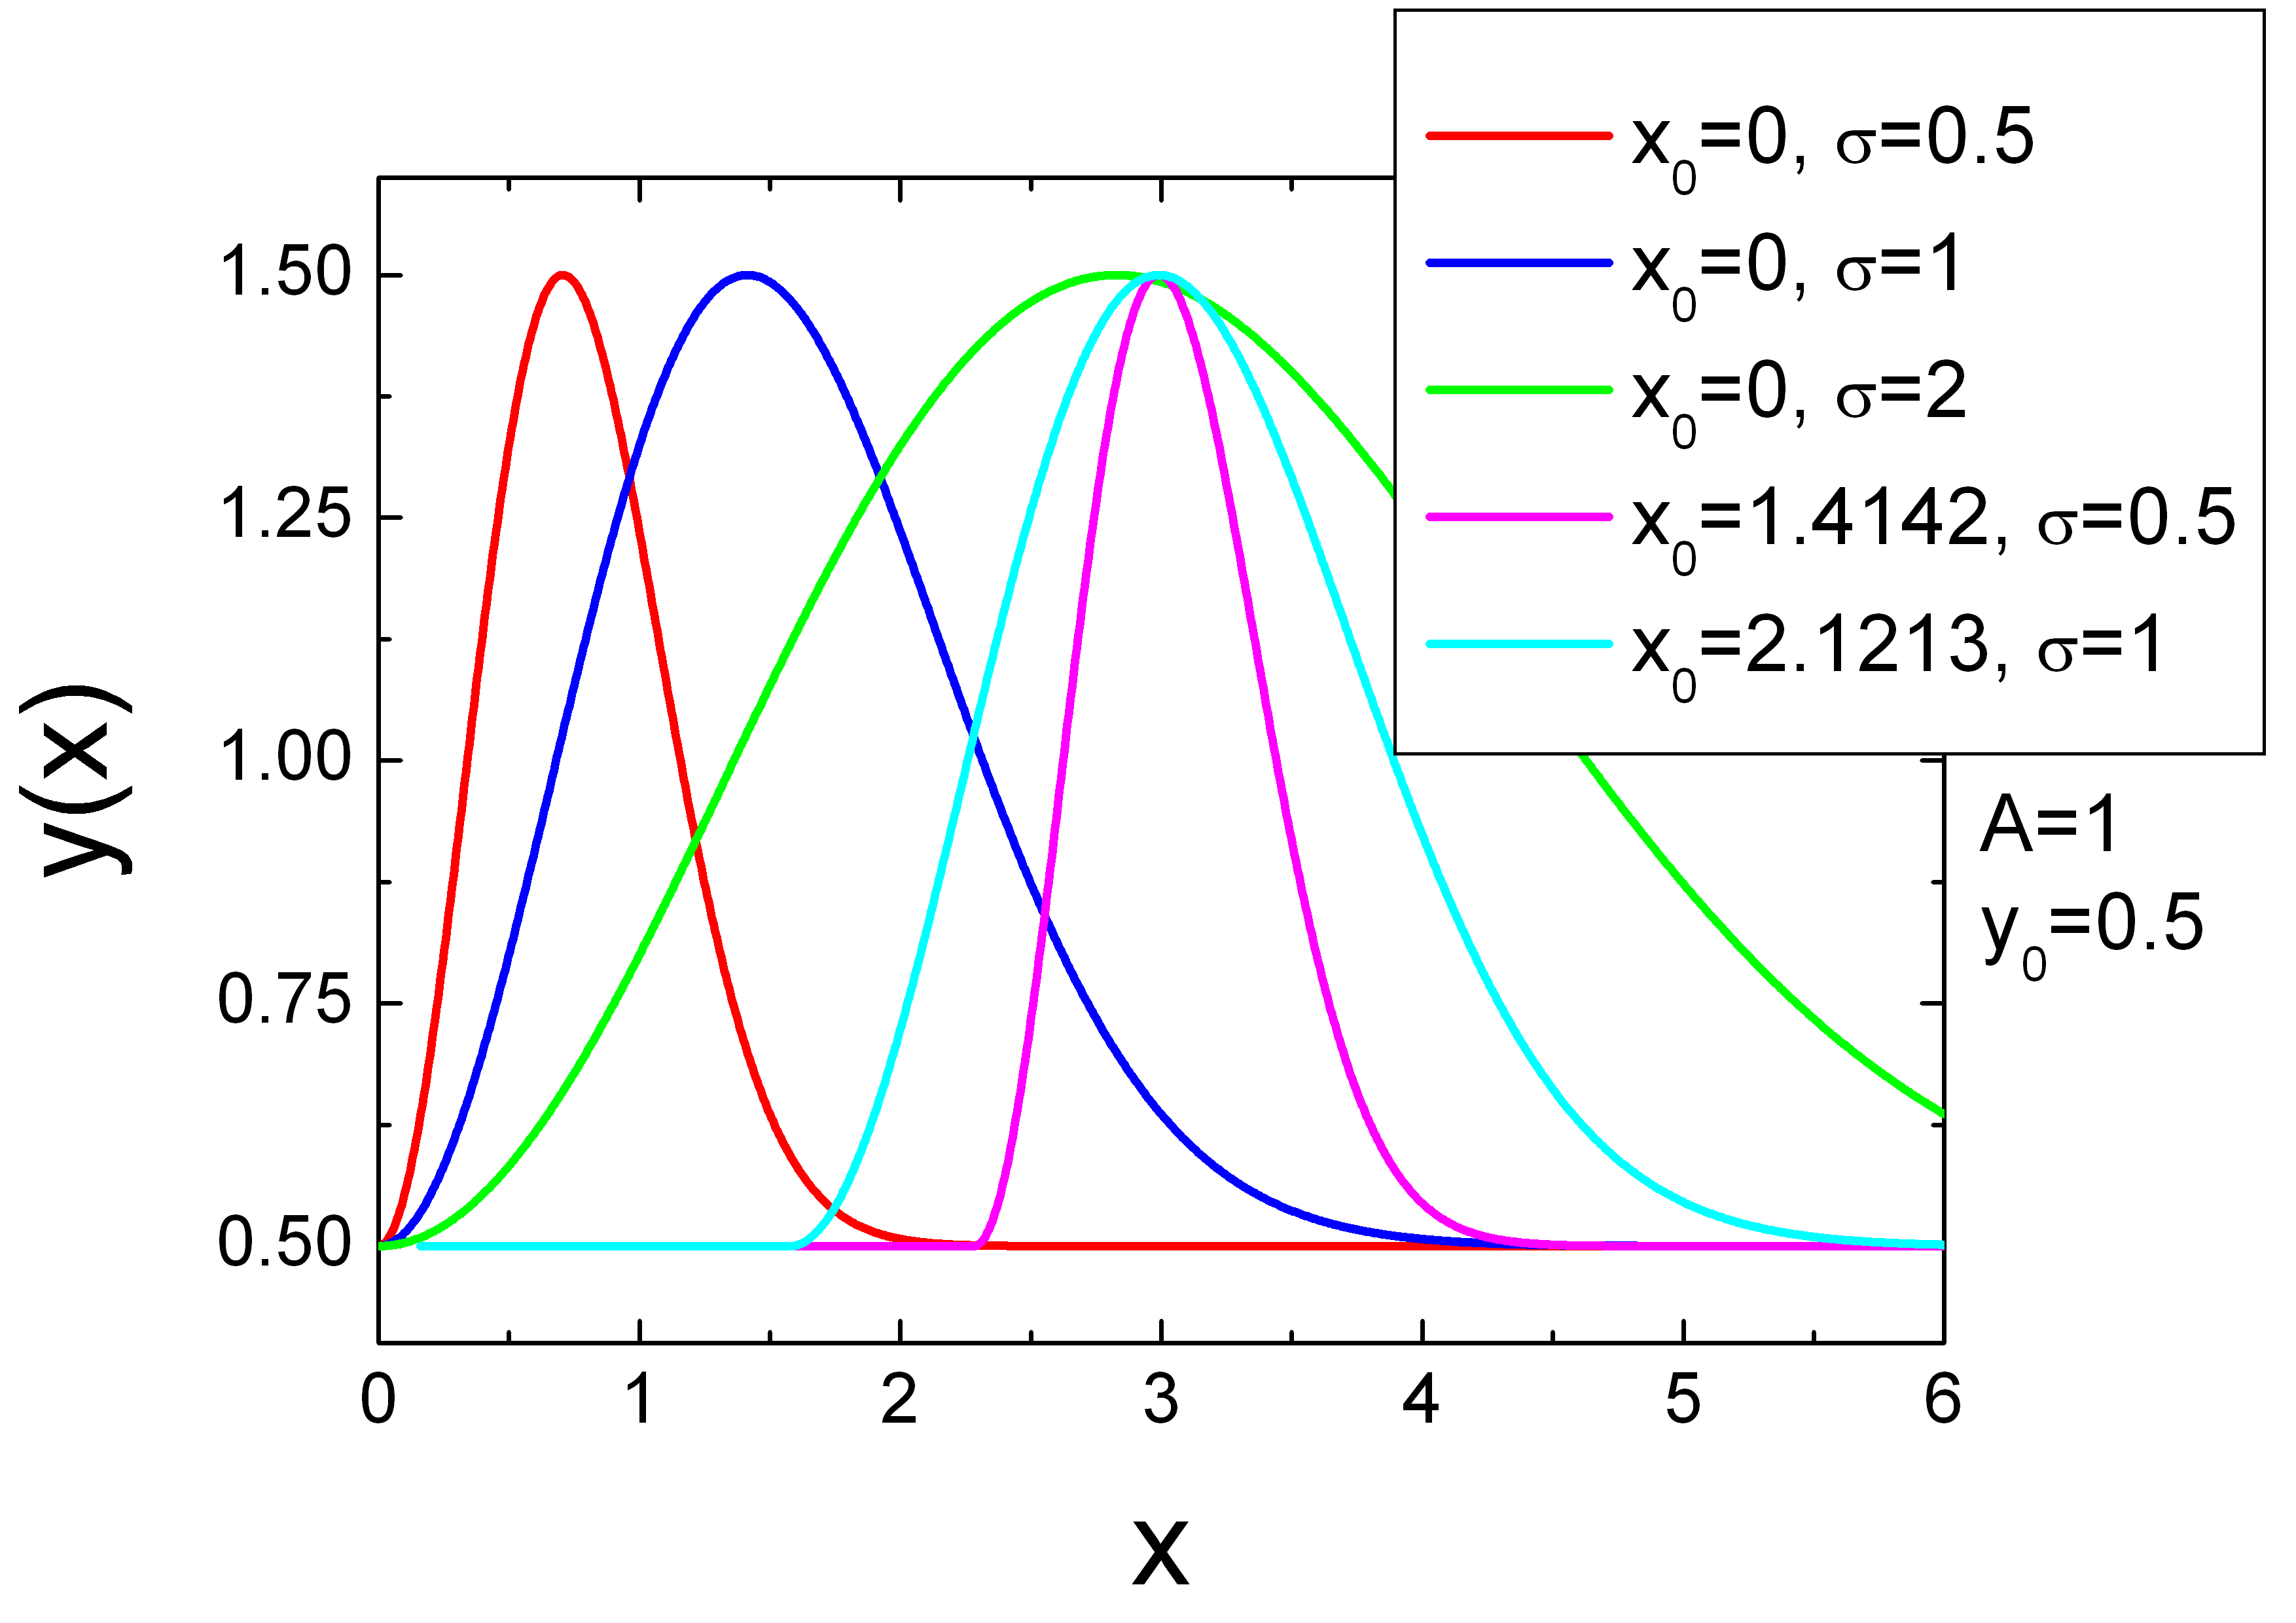
\includegraphics[width=0.6824\textwidth]{MaxwellAmplitude.png}
\end{center}
\caption{Plot of \texttt{Maxwell (Amplitude)} distribution.}
\label{fig:MaxwellAmplitude}
\end{figure}

%%%%%%%%%%%%%%%%%%%%%%%%%%%%%%%%%%%%%%%%%%%%%%%%%%%%%%%%%%%%%%%%%%%%%%%%%%%%%%%%
\clearpage
\subsection{Maxwell (Area)} ~\\
\label{sec:MaxwellArea}

\begin{align}
y(x;A,\sigma,x_0,y_0) &=
\begin{cases}
y_0 & \mbox{for~} x < x_0 \\
y_0 +  \sqrt{\frac{2}{\pi}} \frac{A\left(x-x_0\right)^2}{\sigma^3}
        \exp\left(-\frac{1}{2}\left(\frac{x-x_0}{\sigma}\right)^2\right)
& \mbox{for~} x \geq x_0
\end{cases}
\end{align}

\begin{figure}[htb]
\begin{center}
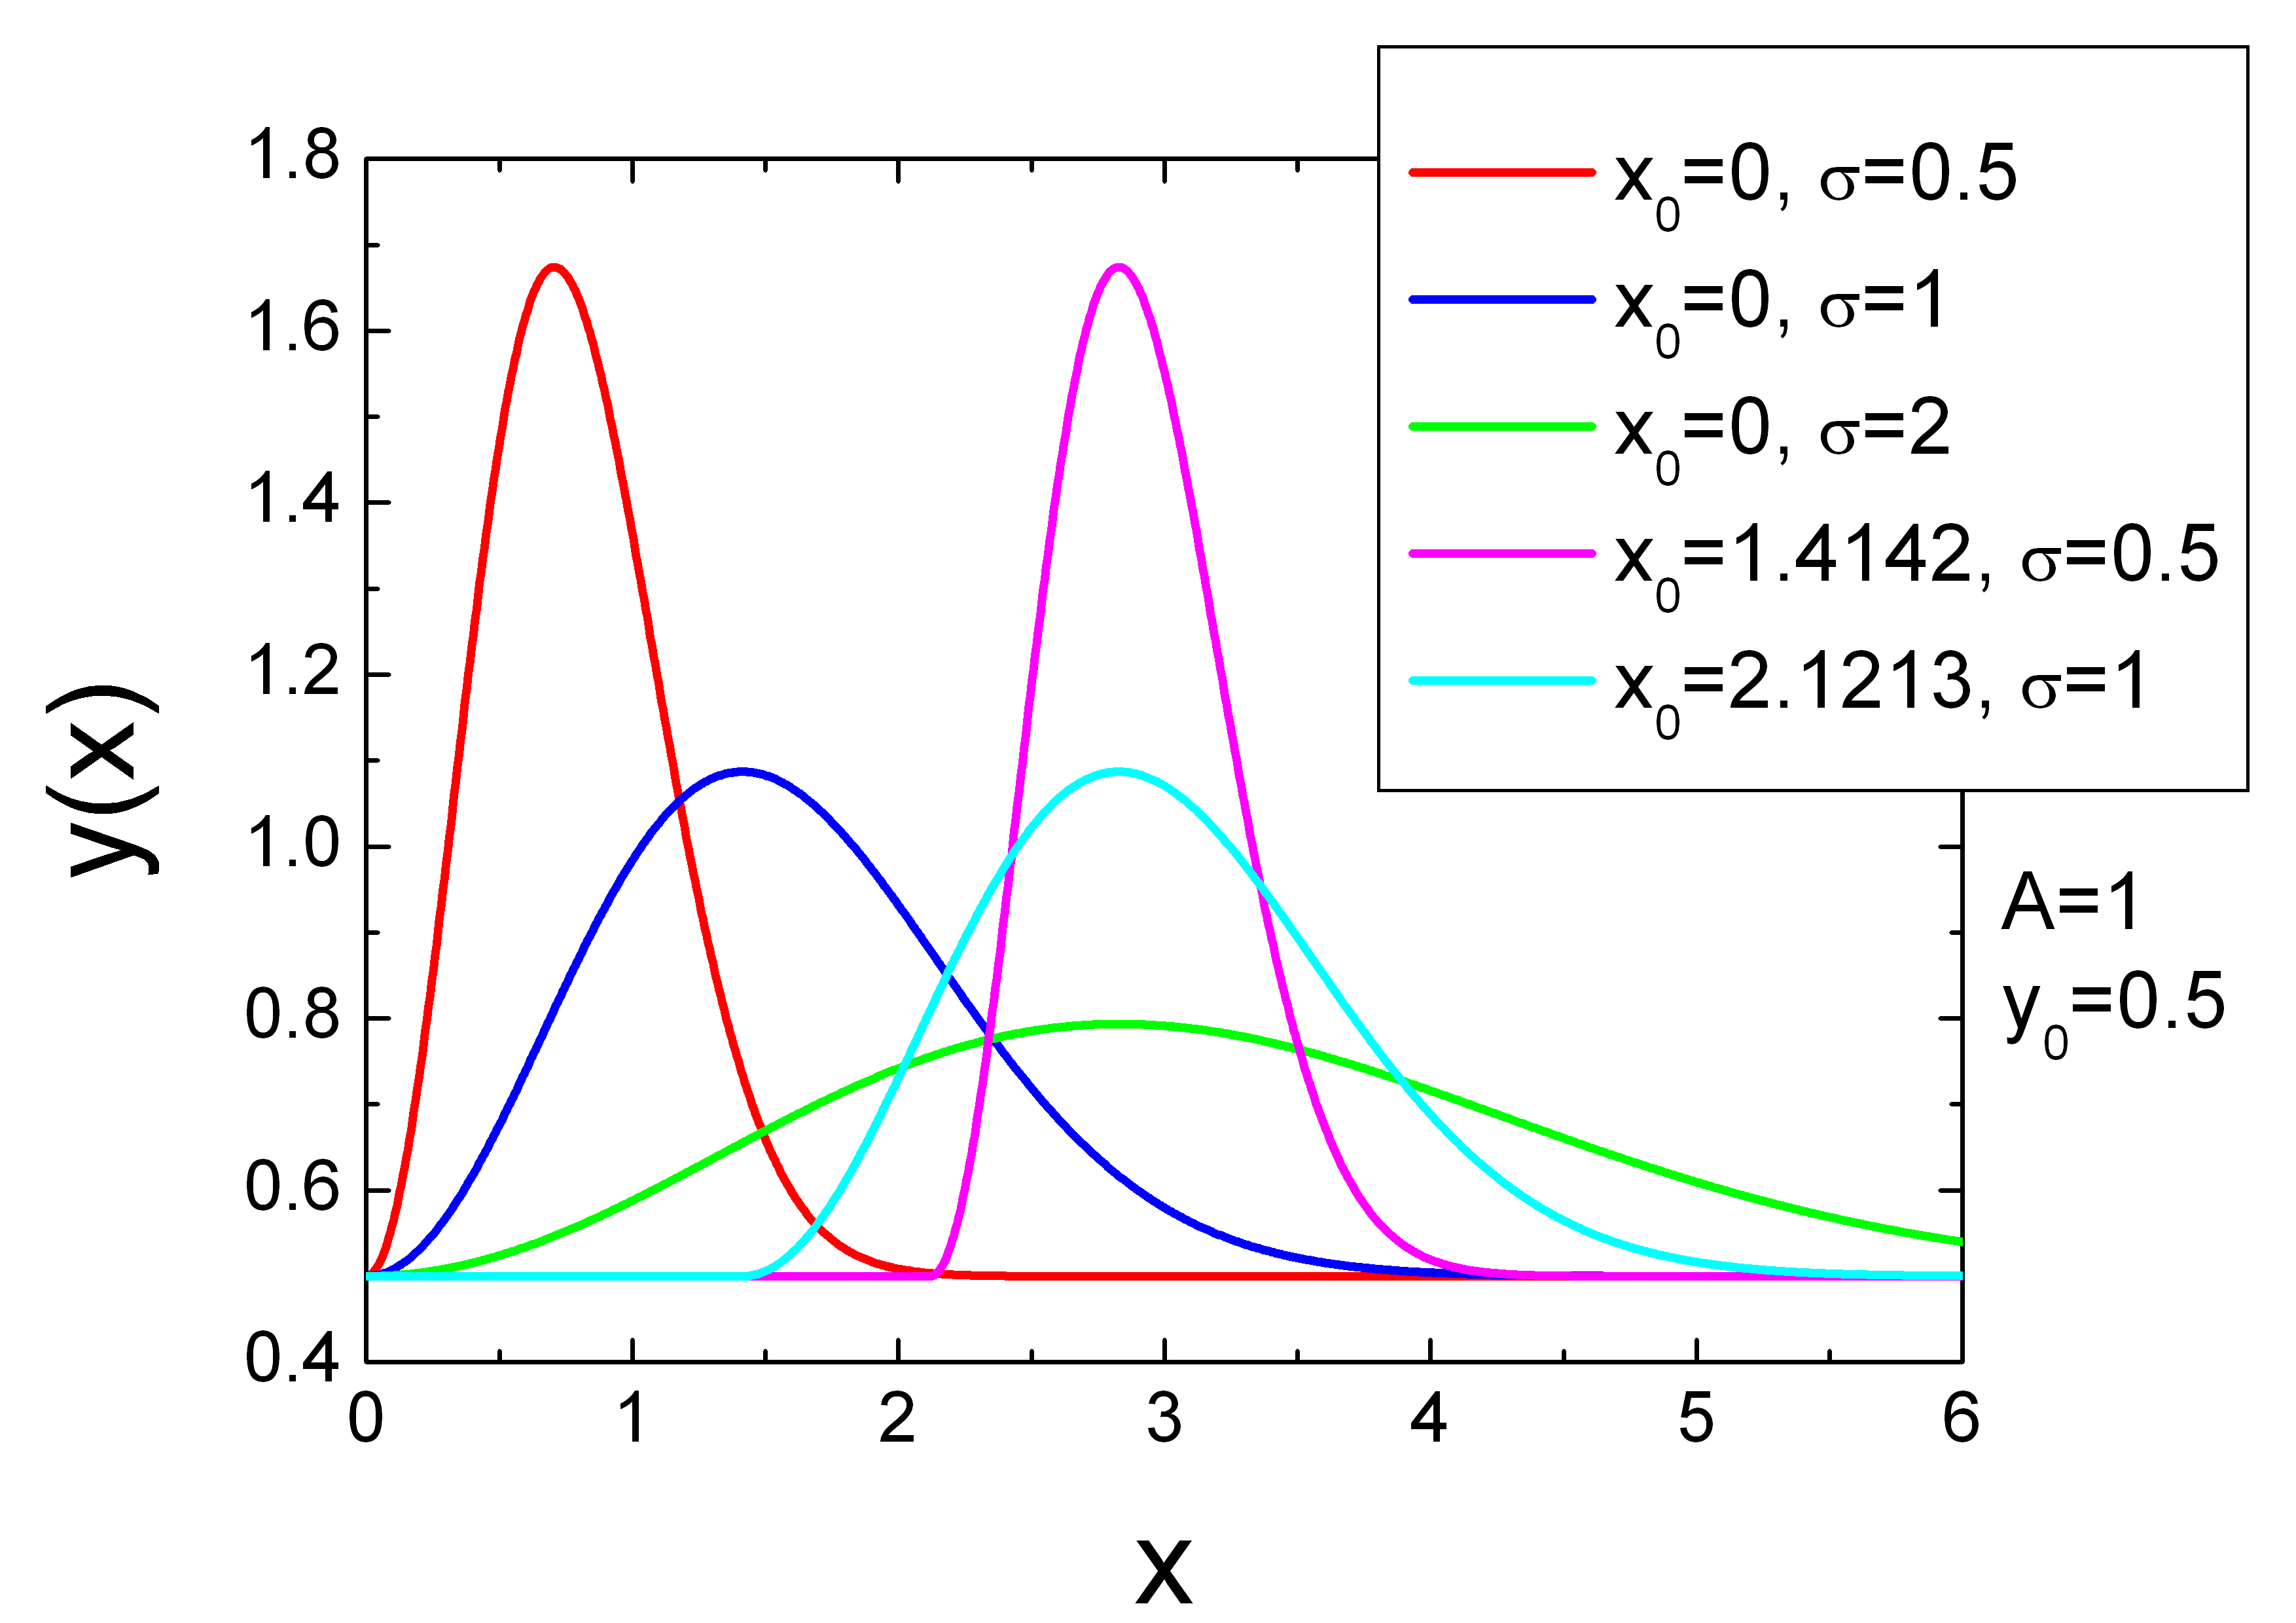
\includegraphics[width=0.6824\textwidth]{MaxwellArea.png}
\end{center}
\caption{Plot of \texttt{Maxwell (Area)} distribution.}
\label{fig:MaxwellArea}
\end{figure}

\clearpage
\subsection{generalized Maxwell (Amplitude)} ~\\
\label{sec:generalizedMaxwellAmplitude}

\begin{align}
y(x; x_0, \sigma, n, m) &=
\begin{cases}
y_0 & \mbox{for~} x<x_0 \\
y_0+ A\; \frac{\left(x-x_0\right)^m
\exp\left(-\frac{1}{2}\left(\frac{x-x_0}{\abs{\sigma}}\right)^n\right)}{
    \left(x_\text{mode}-x_0\right)^m
\exp\left(-\frac{1}{2}\left(\frac{x_\text{mode}-x_0}{\abs{\sigma}}\right)^n\right)}
   & \mbox{for~} x \geq x_0 \\
\end{cases}
\end{align}
with $x_\text{mode} = \left(\frac{2m}{n}\right)^{1/n}\abs{\sigma}+x_0$.

\begin{figure}[htb]
\begin{center}
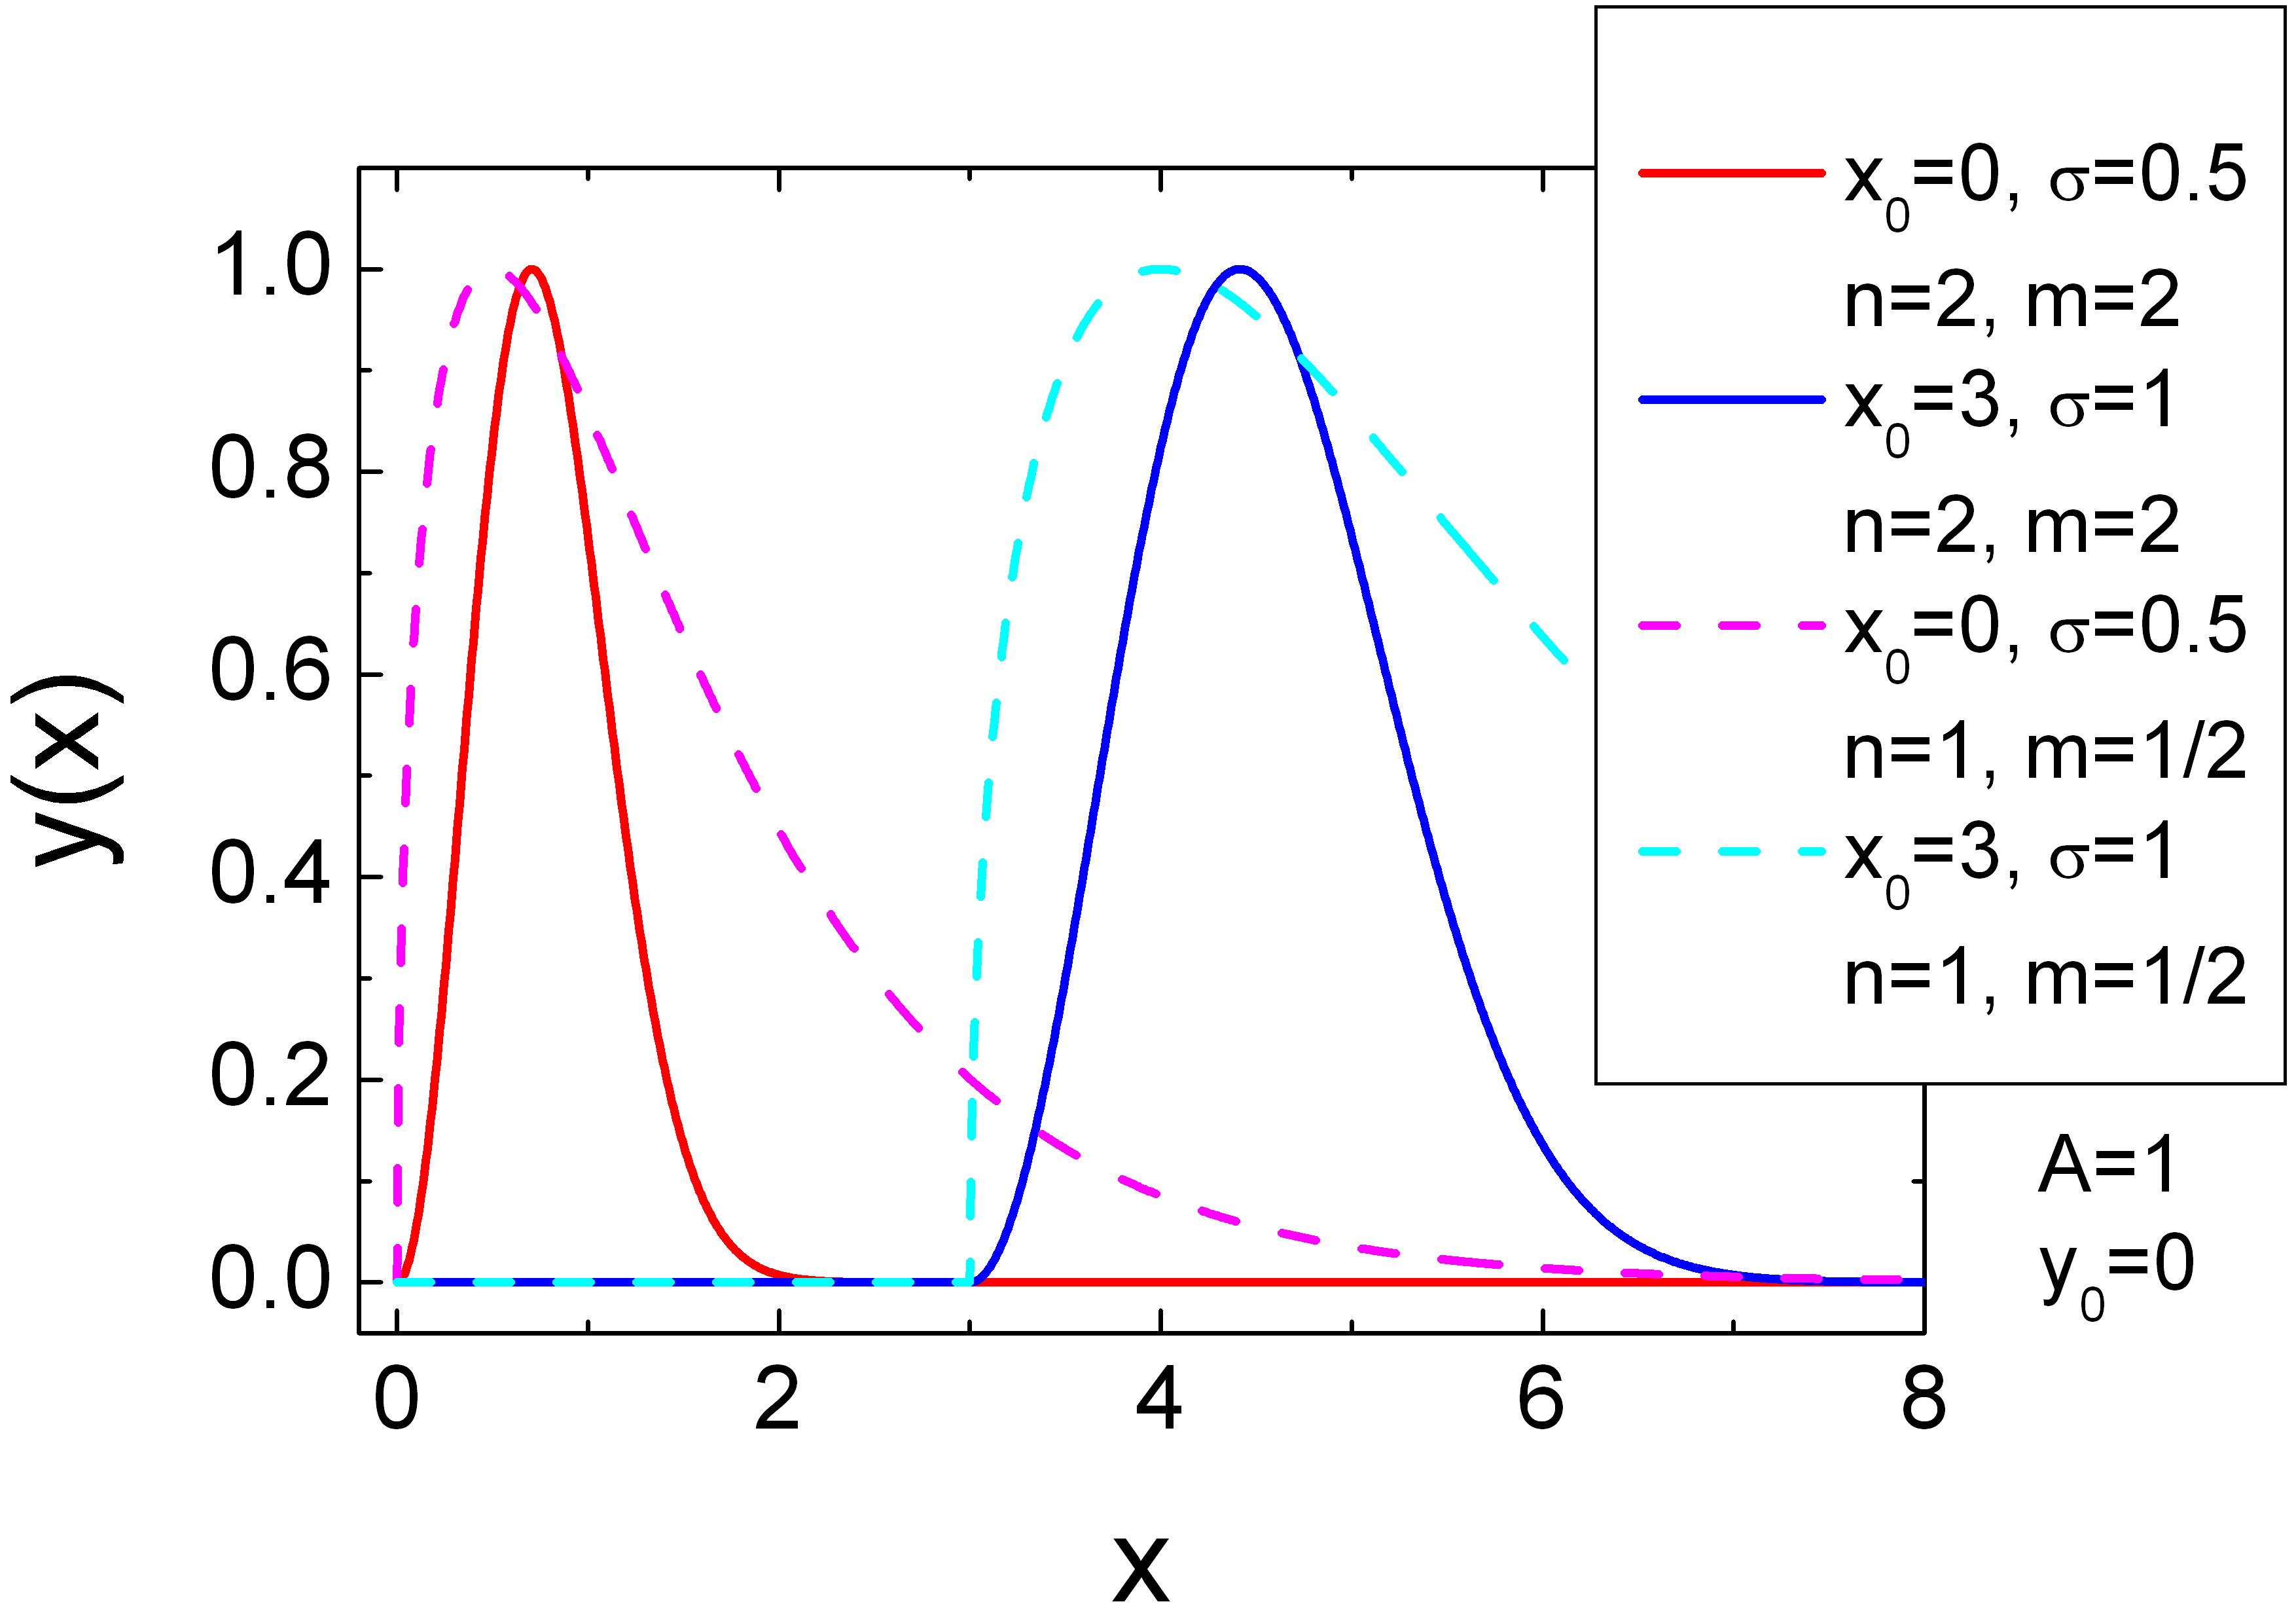
\includegraphics[width=0.6824\textwidth]{generalizedMaxwellAmplitude.png}
\end{center}
\caption{Plot of \texttt{generalized Maxwell (Amplitude)}
distribution.} \label{fig:generalizedMaxwellAmplitude}
\end{figure}

%%%%%%%%%%%%%%%%%%%%%%%%%%%%%%%%%%%%%%%%%%%%%%%%%%%%%%%%%%%%%%%%%%%%%%%%%%%%%%%%
\clearpage
\subsection{generalized Maxwell (Area)} ~\\
\label{sec:generalizedMaxwellArea}

\begin{align}
y(x; x_0, \sigma, n, m) &=
\begin{cases}
0 & \mbox{for~} x<x_0 \\
   A\; \frac{\left(x-x_0\right)^m \exp\left(-\frac{1}{2}\left(\frac{x-x_0}{\abs{\sigma}}\right)^n\right)}{
   2^{(1+m)/n}\abs{\sigma}^{1+m} \frac{1}{\abs{n}}\Gamma\left(\frac{1+m}{n}\right)}
   & \mbox{for~} x \geq x_0 .\\
\end{cases}
\end{align}

\begin{figure}[htb]
\begin{center}
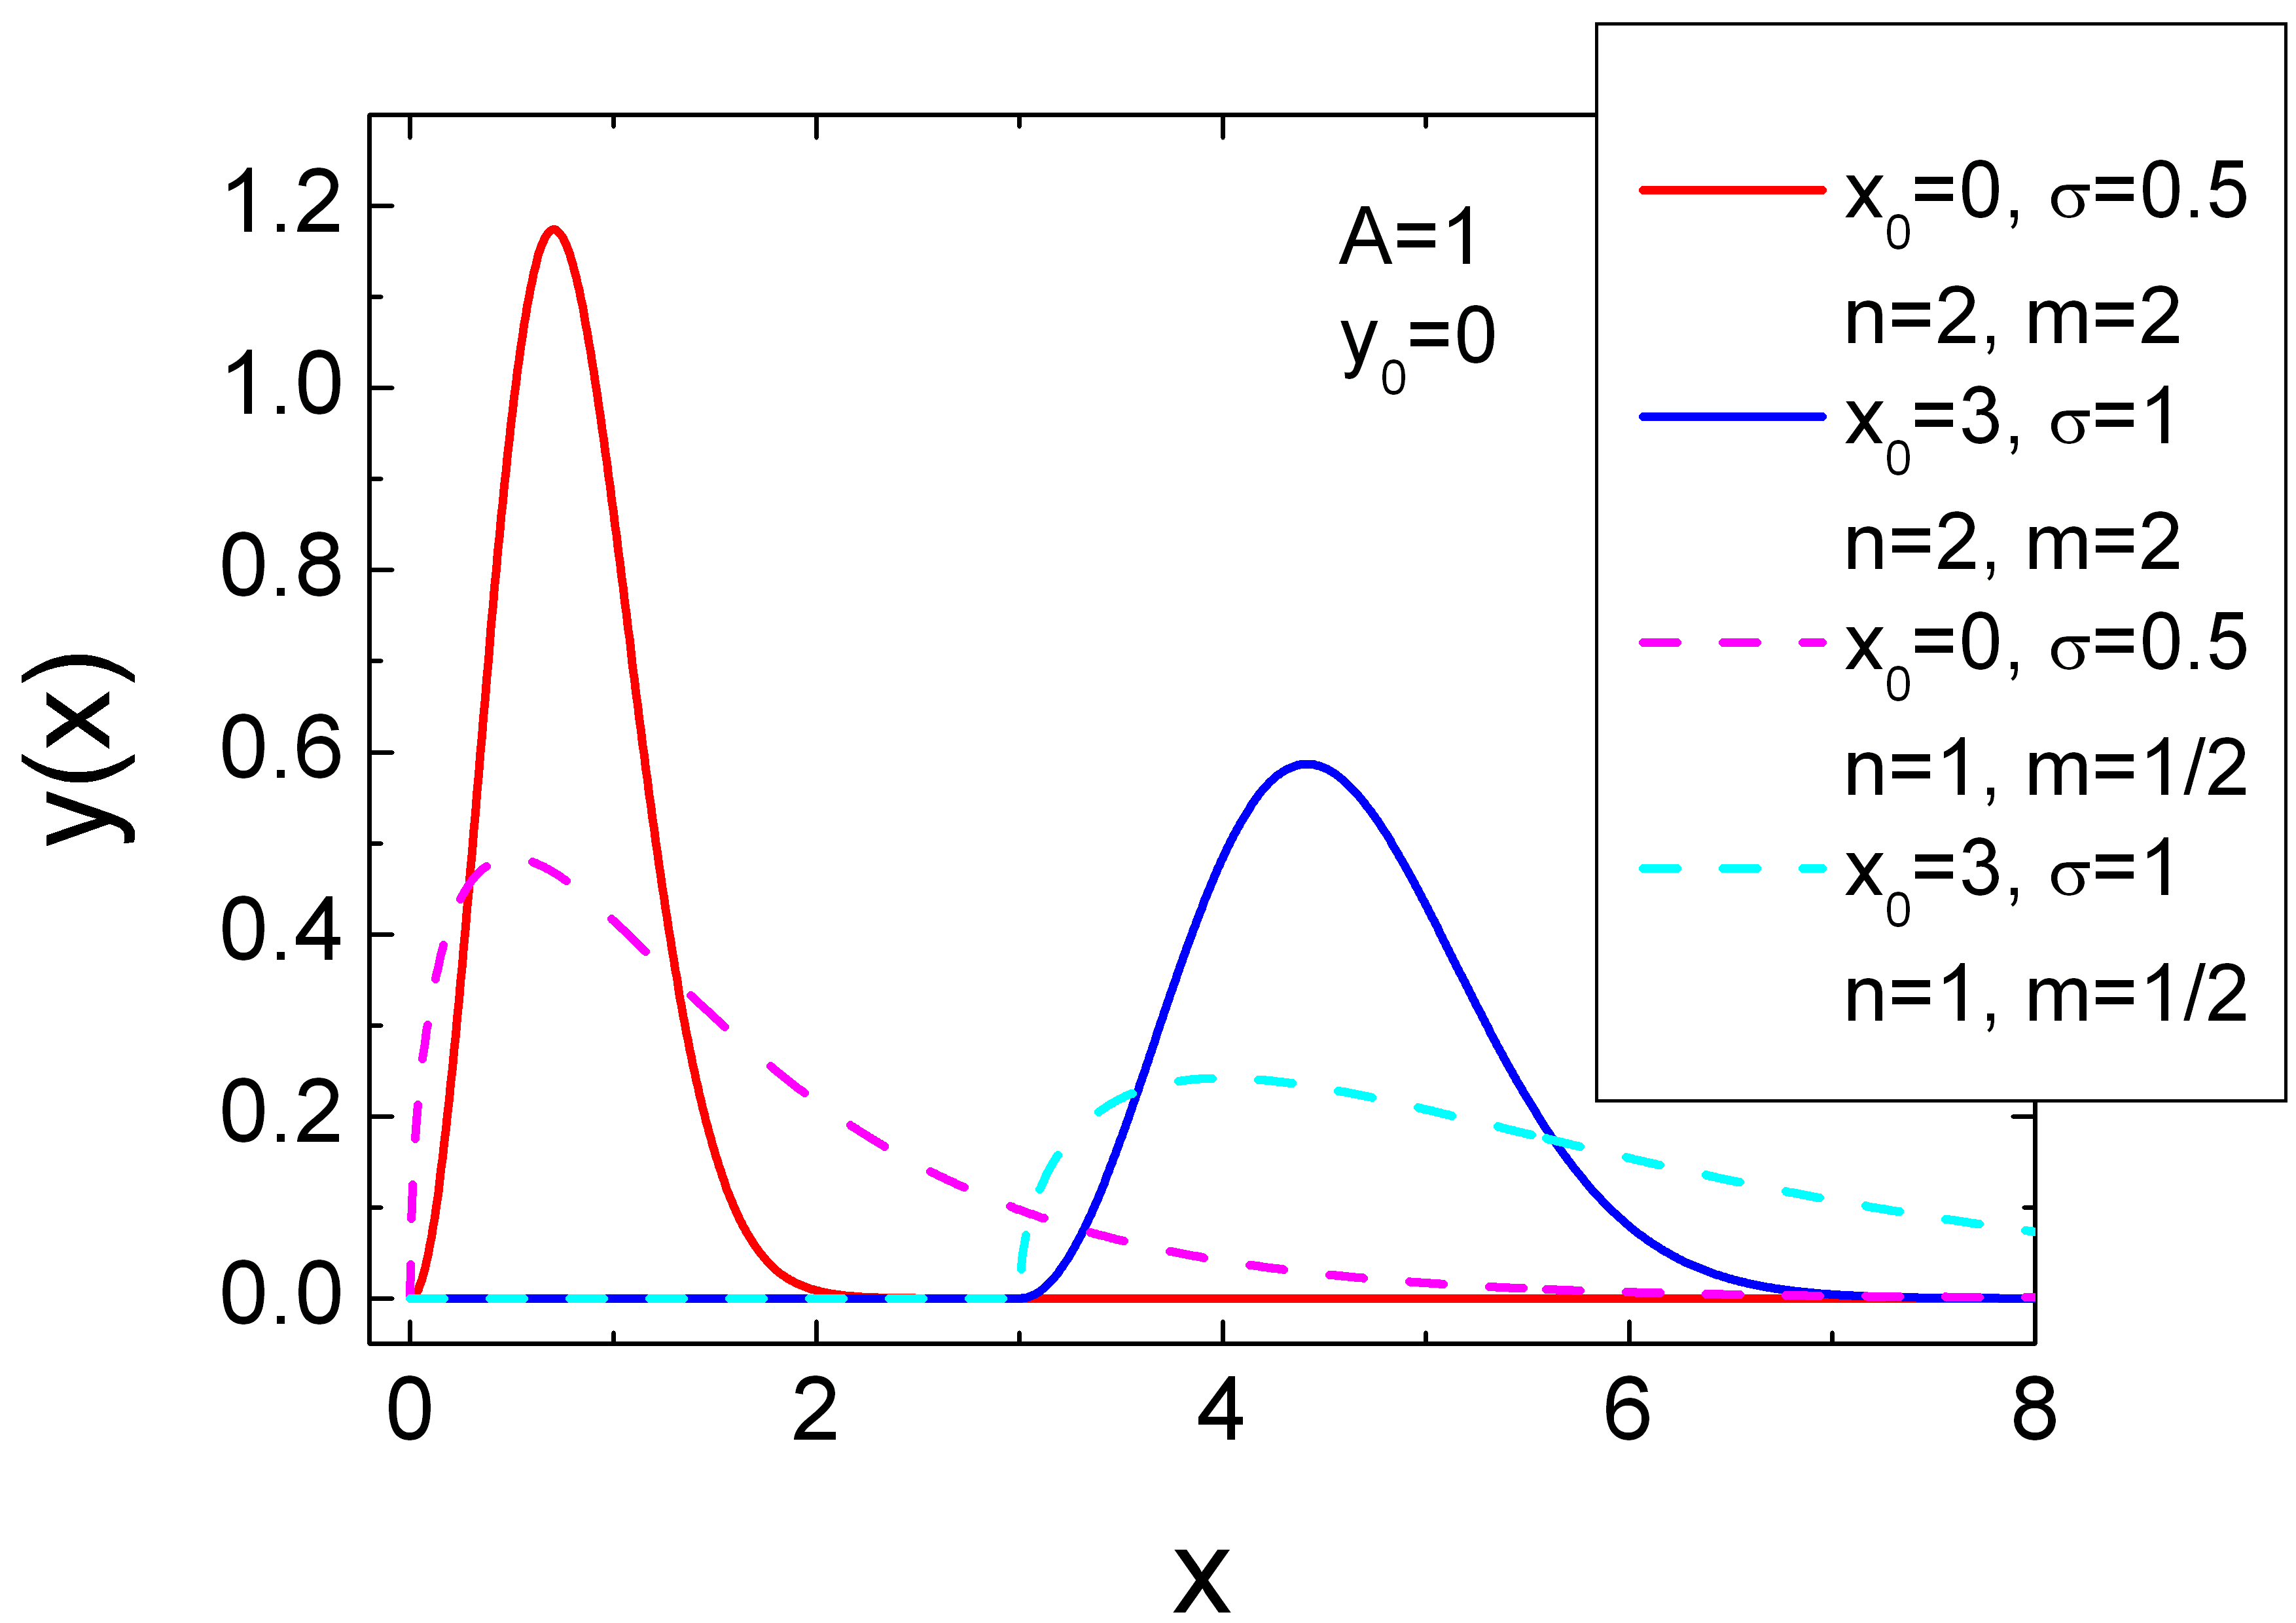
\includegraphics[width=0.6824\textwidth]{generalizedMaxwellArea.png}
\end{center}
\caption{Plot of \texttt{generalized Maxwell (Area)}
distribution.} \label{fig:generalizedMaxwellArea}
\end{figure}



%%%%%%%%%%%%%%%%%%%%%%%%%%%%%%%%%%%%%%%%%%%%%%%%%%%%%%%%%%%%%%%%%%%%%%%%%%%%%%%%
\clearpage
\section{Pearson-IV} ~\\
\label{sec:PearsonIV}
 Pearson type IV distribution:
\begin{align}
    p(x) &= \frac{\left|\frac{\Gamma\!\left(m+\frac{\nu}{2}i\right)}{\Gamma(m)}\right|^2} {\alpha\,\mathrm{B}\!\left(m-\frac12, \frac12\right)} \left[1 + \left(\frac{x-\lambda}{\alpha}\right)^{\!2\,} \right]^{-m} \exp\left[-\nu \arctan\left(\frac{x-\lambda}{\alpha}\right)\right]. \!
\end{align}
The normalizing constant involves the complex Gamma function ($\Gamma$) and the Beta function ($\mathrm{B}$).
For the distribution the mode, mean and variance are given by
\begin{align}
\mathrm{mode} &= \mathcal{M} = \lambda-\frac{\alpha\nu}{2m} \\
\mathrm{mean} &= \langle x \rangle = \lambda-\frac{\alpha\nu}{2(m-1)} \qquad ((m>1)) \\
\mathrm{variance} &= \langle (x-\langle x \rangle)^2 \rangle = \frac{\alpha^2}{r^2(r-1)} \left(r^2+\nu^2 \right)\mbox{ for } m>\frac{3}{2} \\
& \mbox{ with } r=2(m-1) \nonumber
\end{align}
The shape parameter $\nu$ of the Pearson type IV distribution controls its skewness. If we fix its value at zero, we obtain a symmetric three-parameter family. This special case is known as the Pearson type VII distribution \ref{sec:PearsonVII}.
\subsection{Pearson-IV (Amplitude)} ~\\
\label{sec:PearsonIVAmplitude}
\begin{figure}[htb]
\begin{center}
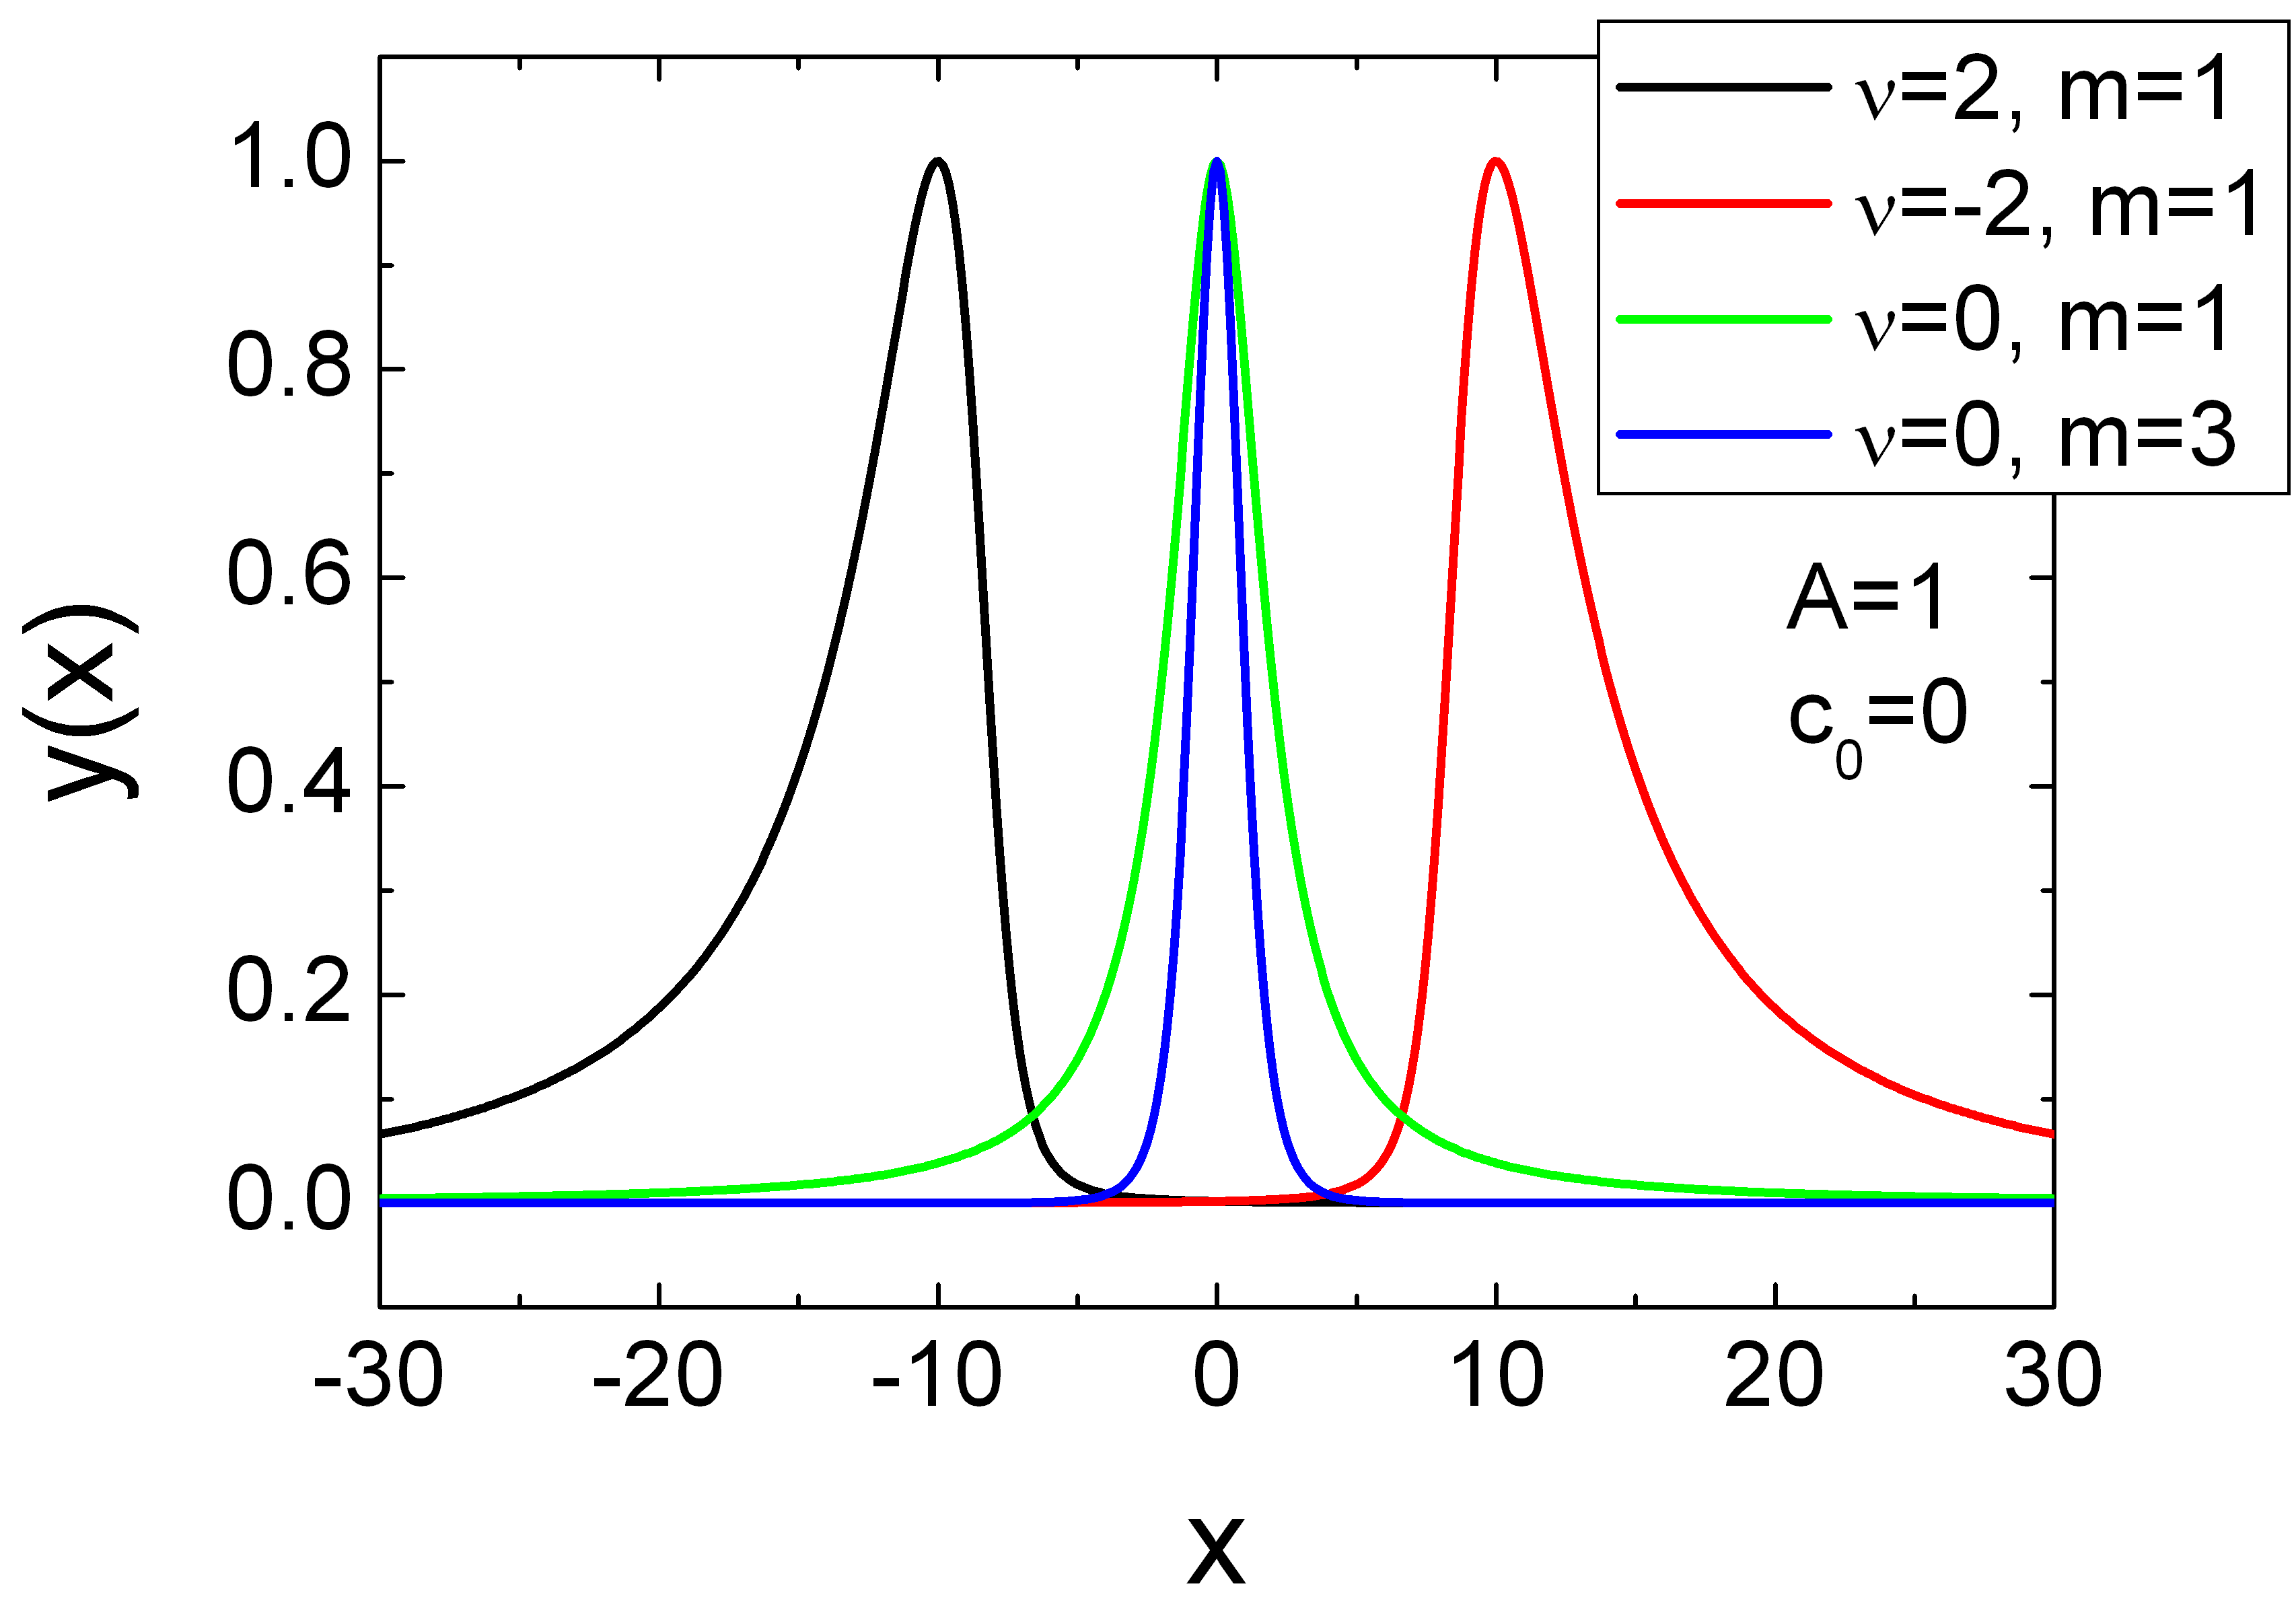
\includegraphics[width=0.6824\textwidth]{PearsonIVAmplitude.png}
\end{center}
\caption{Plot of \texttt{Pearson-IV (Amplitude)} distribution.}
\label{fig:PearsonIVAmplitude}
\end{figure}
%%%%%%%%%%%%%%%%%%%%%%%%%%%%%%%%%%%%%%%%%%%%%%%%%%%%%%%%%%%%%%%%%%%%%%%%%%%%%%%%
\clearpage
\subsection{Pearson-IV (Area)} ~\\
\label{sec:PearsonIVArea}
\begin{figure}[htb]
\begin{center}
\includegraphics[width=0.6824\textwidth]{PearsonIVArea.png}
\end{center}
\caption{Plot of \texttt{Pearson-IV (Area)} distribution.}
\label{fig:PearsonIVArea}
\end{figure}
%%%%%%%%%%%%%%%%%%%%%%%%%%%%%%%%%%%%%%%%%%%%%%%%%%%%%%%%%%%%%%%%%%%%%%%%%%%%%%%%
\clearpage
\section{Pearson-VII} ~\\
\label{sec:PearsonVII}
The \texttt{Pearson-VII} model has been used as
an approximation for the \texttt{Voigt} function.
The parameter $\sigma$ is the FWHM (full-width at half-maxima). When
$m$ is 1.0, the function is an exact Lorentzian. As the $m$-power term
increases, the function tends toward the Gaussian. For $m\sim 50$, the
function is essentially Gaussian. The \texttt{Pearson VII} function is a different
parametrization of the Student-t distribution function and reads as
\begin{align}
    p(x) &= \frac{1}{\alpha\,\mathrm{B}\!\left(m-\frac12, \frac12\right)}
        \left[1 + \left(\frac{x-\lambda}{\alpha}\right)^{\!2\,} \right]^{-m}
\end{align}
where B is the Beta function $\mathrm{B}(a,b)=\Gamma(a)\Gamma(b)/\Gamma(a+b)$, with $a$ and $b$ not being negative integers. The mode $\mathcal{M}$ of the distribution is equals $\mathcal{M} = \lambda$.

Sometimes distribution function are described by the mode $\mathcal{M}$ and integral peak width or peak breadth $\beta$. The peak breadth is given by $\beta=p(\mathcal{M})/\int_{\infty}^\infty p(x)\, \mathrm{d}x = \alpha\,\mathrm{B}\left(m-\frac12, \frac12\right)$, so that
\begin{align}
    p(x) &= \frac{1}{\beta}
        \left[1 + \mathrm{B}^2\left(m-\frac12, \frac12\right)\left(\frac{x-\mathcal{M}}{\beta}\right)^{\!2\,} \right]^{-m}
\end{align}

An alternative parameterization (and slight specialization) of the type VII distribution is obtained by letting
$\alpha=\sigma\sqrt{2m-3}$, which requires $m > 3/2$. By this constrain the variance of the distribution exists and is equal to $\sigma^2$.
\begin{align}
    p(x) &=  \frac{1}{\sigma\,\sqrt{2\,m-3}\,\mathrm{B}\!\left(m-\frac12, \frac12\right)} \left[1 + \left(\frac{x-\lambda}{\sigma\,\sqrt{2\,m-3}}\right)^{\!2\,} \right]^{-m}
\end{align}
Now the parameter $m$ only controls the kurtosis of the distribution. If $m$ approaches infinity as $\lambda$
and $\sigma$ are held constant, the normal distribution arises as a special case:
\begin{align}
& \lim_{m\to\infty}\frac{1}{\sigma\,\sqrt{2\,m-3}\,\mathrm{B}\!\left(m-\frac12, \frac12\right)} \left[1 + \left(\frac{x-\lambda}{\sigma\,\sqrt{2\,m-3}}\right)^{\!2\,} \right]^{-m} \nonumber\\
& = \frac{1}{\sigma\,\sqrt{2}\,\Gamma\!\left(\frac12\right)} \times \lim_{m\to\infty} \frac{\Gamma(m)}{\Gamma\!\left(m-\frac12\right) \sqrt{m-\frac32}} \times \lim_{m\to\infty} \left[1 + \frac{\left(\frac{x-\lambda}{\sigma}\right)^2}{2\,m-3} \right]^{-m} \nonumber\\
& = \frac{1}{\sigma\sqrt{2\,\pi}} \times 1 \times \exp\!\left[-\frac12 \left(\frac{x-\lambda}{\sigma}\right)^{\!2\,} \right] \nonumber
\end{align}
For $m>\frac52$ the distribution could also be expressed in terms of excess kurtosis $\gamma_2$ or kurtosis $\kappa$ by letting
\begin{align}
m =& \frac52+\frac{3}{\gamma_2} \\
\mbox{or } m =& \frac52+\frac{3}{\kappa-3}
\end{align}

It is also possible to express the Pearson distribution in terms of the full width of half maximum $\omega_\mathrm{FWHM}$ by substituting $\alpha=\omega_\mathrm{FWHM}/\left(2\sqrt{2^{1/m}-1}\right)$. This leads to
\begin{align}
    p(x) &= \frac{2\sqrt{2^{1/m}-1}}{\omega_\mathrm{FWHM}\,\mathrm{B}\!\left(m-\frac12, \frac12\right)}
        \left[1 + 4\left(\sqrt{2^{1/m}-1}\right)\left(\frac{x-\lambda}{\omega_\mathrm{FWHM}}\right)^{\!2\,} \right]^{-m}
\end{align}

\clearpage
\subsection{Pearson-VII (Amplitude)} ~\\
\label{sec:PearsonVIIAmplitude}
\begin{figure}[htb]
\begin{center}
\includegraphics[width=0.6824\textwidth]{PearsonVIIAmplitude.png}
\end{center}
\caption{Plot of \texttt{Pearson-VII (Amplitude)} distribution.}
\label{fig:PearsonVIIAmplitude}
\end{figure}

%%%%%%%%%%%%%%%%%%%%%%%%%%%%%%%%%%%%%%%%%%%%%%%%%%%%%%%%%%%%%%%%%%%%%%%%%%%%%%%%
\clearpage
\subsection{Pearson-VII (Area)} ~\\
\label{sec:PearsonVIIArea}
\begin{figure}[htb]
\begin{center}
\includegraphics[width=0.6824\textwidth]{PearsonVIIArea.png}
\end{center}
\caption{Plot of \texttt{Pearson-VII (Area)} distribution.}
\label{fig:PearsonVIIArea}
\end{figure}

%%%%%%%%%%%%%%%%%%%%%%%%%%%%%%%%%%%%%%%%%%%%%%%%%%%%%%%%%%%%%%%%%%%%%%%%%%%%%%%%
\clearpage
\section{Pulse Peak} ~\\
\label{sec:Pulse}
\begin{align}
p(x) &= \frac{2}{\sigma}\exp\left(\frac{x-x_0}{\sigma}\right) \left(1-\exp\left(\frac{x-x_0}{\sigma}\right)\right)
\end{align}
\begin{align}
\mbox{mode} &= x_0 - \sigma \ln\left(\frac12\right)
\end{align}
\subsection{Pulse Peak (Amplitude)} ~\\
\label{sec:PulseAmplitude}

\begin{figure}[htb]
\begin{center}
\includegraphics[width=0.6824\textwidth]{PulseAmplitude.png}
\end{center}
\caption{Plot of \texttt{Pulse Peak (Amplitude)} distribution.}
\label{fig:PulseAmplitude}
\end{figure}

%%%%%%%%%%%%%%%%%%%%%%%%%%%%%%%%%%%%%%%%%%%%%%%%%%%%%%%%%%%%%%%%%%%%%%%%%%%%%%%%
\clearpage
\subsection{Pulse Peak (Area)} ~\\
\label{sec:PulseArea}

\begin{figure}[htb]
\begin{center}
\includegraphics[width=0.6824\textwidth]{PulseArea.png}
\end{center}
\caption{Plot of \texttt{Pulse Peak (Area)} distribution.}
\label{fig:PulseArea}
\end{figure}

%%%%%%%%%%%%%%%%%%%%%%%%%%%%%%%%%%%%%%%%%%%%%%%%%%%%%%%%%%%%%%%%%%%%%%%%%%%%%%%%
\clearpage
\section{Pulse Peak with 2nd Width Term} ~\\
\label{sec:pulsewith2ndwidth}
\begin{align}
p(x) &= \frac{\sigma_1+\sigma_2}{\sigma_2^2} \left(1-\exp\left(\frac{x-x_0}{\sigma_1}\right)\right) \exp\left(\frac{x-x_0}{\sigma_2}\right)
\end{align}
\begin{align}
\mbox{mode} &= x_0 - \sigma_1 \ln\left(\frac{\sigma_1}{\sigma_2+\sigma_1}\right)
\end{align}

\subsection{Pulse Peak with 2nd Width Term (Amplitude)} ~\\
\label{sec:pulsewith2ndwidthAmplitude}

\begin{figure}[htb]
\begin{center}
\includegraphics[width=0.6824\textwidth]{Pulse2ndWidthAmplitude.png}
\end{center}
\caption{Plot of \texttt{pulse with 2nd width (Amplitude)} distribution.}
\label{fig:Pulse2ndWidthAmplitude}
\end{figure}

%%%%%%%%%%%%%%%%%%%%%%%%%%%%%%%%%%%%%%%%%%%%%%%%%%%%%%%%%%%%%%%%%%%%%%%%%%%%%%%%
\clearpage
\subsection{Pulse Peak with 2nd Width Term (Area)} ~\\
\label{sec:pulsewith2ndwidthArea}

\begin{figure}[htb]
\begin{center}
\includegraphics[width=0.6824\textwidth]{Pulse2ndWidthArea.png}
\end{center}
\caption{Plot of \texttt{pulse with 2nd width (Area)} distribution.}
\label{fig:Pulse2ndWidthArea}
\end{figure}

%%%%%%%%%%%%%%%%%%%%%%%%%%%%%%%%%%%%%%%%%%%%%%%%%%%%%%%%%%%%%%%%%%%%%%%%%%%%%%%%
\clearpage
\section{Pulse Peak with Power Term} ~\\
\label{sec:pulsewithpowerterm}
\begin{align}
p(x) &= \frac{\gamma+1}{\sigma} \left(1-\exp\left(\frac{x-x_0}{\sigma}\right)\right)^\gamma \exp\left(\frac{x-x_0}{\sigma}\right)
\end{align}
\begin{align}
\mbox{mode} &= x_0 - \sigma \ln\left(\frac{1}{\gamma+1}\right)
\end{align}

\subsection{Pulse Peak with Power Term (Amplitude)} ~\\
\label{sec:pulsewithpowertermAmplitude}

\begin{figure}[htb]
\begin{center}
\includegraphics[width=0.6824\textwidth]{PulsePowerAmplitude.png}
\end{center}
\caption{Plot of \texttt{pulse with power term (Amplitude)} distribution.}
\label{fig:PulsePowerAmplitude}
\end{figure}

%%%%%%%%%%%%%%%%%%%%%%%%%%%%%%%%%%%%%%%%%%%%%%%%%%%%%%%%%%%%%%%%%%%%%%%%%%%%%%%%
\clearpage
\subsection{Pulse Peak with Power Term (Area)} ~\\
\label{sec:pulsewithpowertermArea}

\begin{figure}[htb]
\begin{center}
\includegraphics[width=0.6824\textwidth]{PulsePowerArea.png}
\end{center}
\caption{Plot of \texttt{pulse with power term (Area)} distribution.}
\label{fig:PulsePowerArea}
\end{figure}

%%%%%%%%%%%%%%%%%%%%%%%%%%%%%%%%%%%%%%%%%%%%%%%%%%%%%%%%%%%%%%%%%%%%%%%%%%%%%%%%
\clearpage
\section{Student-t}
\label{sec:Student-t}
\begin{align}
p(x) &= \frac{\Gamma(\frac{\nu+1}{2})} {\sqrt{\nu\pi}\,\Gamma(\frac{\nu}{2})} \left(1+\frac{x^2}{\nu} \right)^{-(\frac{\nu+1}{2})}
\end{align}

\subsection{Student-t (Amplitude)} ~\\
\label{sec:Student-tAmplitude}
\begin{figure}[htb]
\begin{center}
\includegraphics[width=0.6824\textwidth]{StudenttAmplitude.png}
\end{center}
\caption{Plot of \texttt{Student-t (Amplitude)} distribution.}
\label{fig:Student-tAmplitude}
\end{figure}

%%%%%%%%%%%%%%%%%%%%%%%%%%%%%%%%%%%%%%%%%%%%%%%%%%%%%%%%%%%%%%%%%%%%%%%%%%%%%%%%
\clearpage

\subsection{Student-t (Area)} ~\\
\label{sec:Student-tArea}
\begin{figure}[htb]
\begin{center}
\includegraphics[width=0.6824\textwidth]{StudenttArea.png}
\end{center}
\caption{Plot of \texttt{Student-t (Area)} distribution.}
\label{fig:Student-tArea}
\end{figure}

%%%%%%%%%%%%%%%%%%%%%%%%%%%%%%%%%%%%%%%%%%%%%%%%%%%%%%%%%%%%%%%%%%%%%%%%%%%%%%%%
\clearpage
\section{Voigt} ~\\
\label{sec:Voigt}
The Voigt profile is a spectral line profile found in all branches
of spectroscopy in which a spectral line is broadened by two types
of mechanisms, one of which alone would produce a Gaussian profile
(usually, as a result of the Doppler broadening), and the other
would produce a Lorentzian profile. The Voigt profile is then a
convolution of a Lorentz profile and a Gaussian profile:
\begin{subequations}
\begin{align}
V(x,x_c\vert\sigma,\gamma)& = \int_\infty^\infty D(x'\vert\sigma) \,
                                            L(x-x_c-x'\vert\gamma)\, dx'
\end{align}
where $x-x_c$ is distance from line center $x_c$, $D(x\vert\sigma)$ is the
centered Doppler profile:
\begin{align}
D(x\vert\sigma) & = \frac{e^{-x^2/2\sigma^2}}{\sigma\sqrt{2\pi}}
\end{align}
and $L(x-x_c\vert\gamma)$ is the centered Lorentzian profile:
\begin{align}
L(x-x_c\vert\gamma) & = \frac{\gamma}{\pi((x-x_c)^2+\gamma^2)} .
\end{align}
The defining integral can be evaluated as \cite{David1986,Ida2000}:
\begin{align}
V(x,x_c) & = \frac{\Re[w(z)]}{\sigma\sqrt{2\pi}}
\end{align}
where $\Re[w(z)]$ is the real part of the complex error function
of $z$ and
\begin{align}
z = \frac{x-x_c+i\gamma}{\sigma\sqrt{2}}
\end{align}
\end{subequations}
The full width at half maximum (FWHM) of the Voigt profile can be found from
the widths of the associated Gaussian and Lorentzian widths. The FWHM of the
Gaussian profile is $f_G=2\sigma\sqrt{2\ln(2)}$.
The FWHM of the Lorentzian profile is just $f_L = 2\gamma$.
Define $\phi = f_\mathrm{L} / f_\mathrm{G}$. Then the FWHM of the Voigt profile ($f_\mathrm{V}$) can be estimated as:
\begin{equation}
    f_\mathrm{V}\approx f_\mathrm{G}\left(1-c_0c_1+\sqrt{\phi^2+2c_1\phi+c_0^2c_1^2}\right)
\end{equation}
where $c_0 = 2.0056$ and $c_1 = 1.0593$. This estimate will have a standard deviation of
error of about 2.4 percent for values of $\phi$ between 0 and 10. Note that the above
equation will have the proper behavior in the limit of $\phi=0$ and $\phi=\infty$.
A different approximation was given by \cite{Olivero1977,Liu2001}
\begin{equation}
    f_\mathrm{V}\approx 0.5346 f_\mathrm{L}+\sqrt{0.2166f_\mathrm{L}^2+f_\mathrm{G}^2}
\end{equation}
with an accuracy of 0.02%

%%%%%%%%%%%%%%%%%%%%%%%%%%%%%%%%%%%%%%%%%%%%%%%%%%%%%%%%%%%%%%%%%%%%%%%%%%%%%%%%
\clearpage
\subsection{Voigt (Amplitude)} ~\\[5mm]
\label{sec:VoigtAmplitude}
The amplitude version of the Voigt peak is parameterized as
\begin{equation}
V_\text{Amplitude}(x\vert A,\sigma,\gamma)
= A \, \frac{\DS \int_{-\infty}^\infty \frac{\exp(-u^2)}{\frac{\gamma^2}{2\sigma^2}+\left( \frac{x-x_c}{\sqrt{2}\sigma}-u\right)^2} \, du}{\DS \int_{-\infty}^\infty \frac{\exp(-u^2)}{\frac{\gamma^2}{2\sigma^2}+u^2}\, du}
= A \, \frac{V(x,x_c\vert\sigma,\gamma)}{V(x_c,x_c\vert\sigma,\gamma)}
\end{equation}
~\\

\underline{Required parameters:}
\begin{description}
    \item[ampl.] amplitude $A$ of the Voigt peak
    \item[center] location parameter (mode) $x_c$
    \item[sigma] width of Doppler (Gaussian) contribution $\sigma>0$
    \item[gamma] width of Lorentzian contribution $\gamma>0$
    \item[backgr] offset $c_0$
\end{description}

\underline{Note}
\begin{itemize}
  \item The Doppler (Gaussian) width parameter needs to be larger than 0 $\sigma>0$.
  \item The Lorentzian width parameter needs to be larger than 0 $\gamma>0$.
  \item Default (Size) distribution: Monodisperse
\end{itemize}


\begin{figure}[htb]
\begin{center}
\includegraphics[width=0.768\textwidth]{VoigtAmplitude.png}
\end{center}
\caption{Plot of \texttt{Voigt (Amplitude)} distribution.}
\label{fig:VoigtAmplitude}
\end{figure}


%%%%%%%%%%%%%%%%%%%%%%%%%%%%%%%%%%%%%%%%%%%%%%%%%%%%%%%%%%%%%%%%%%%%%%%%%%%%%%%%
\clearpage

\subsection{Voigt (Area)} ~\\[5mm]
\label{sec:VoigtArea}
The area version of the Voigt peak is parameterized as
\begin{equation}
V_\text{Area}(x\vert A,\sigma,\gamma)
= A \, \frac{\gamma}{2\pi\sqrt{\pi}\sigma^2} \int_{-\infty}^\infty \frac{\exp(-u^2)}{\frac{\gamma^2}{2\sigma^2}+\left( \frac{x-x_c}{\sqrt{2}\sigma}-u\right)^2} \, du
= A \, V(x,x_c\vert\sigma,\gamma)
\end{equation}
~\\

\underline{Required parameters:}
\begin{description}
    \item[area] area $A$ of the Voigt peak
    \item[center] location parameter (mode) $x_c$
    \item[sigma] width of Doppler (Gaussian) contribution $\sigma>0$
    \item[gamma] width of Lorentzian contribution $\gamma>0$
    \item[backgr] offset $c_0$
\end{description}

\underline{Note}
\begin{itemize}
  \item The Doppler (Gaussian) width parameter needs to be larger than 0 $\sigma>0$.
  \item The Lorentzian width parameter needs to be larger than 0 $\gamma>0$.
  \item Default (Size) distribution: Monodisperse
\end{itemize}


\begin{figure}[htb]
\begin{center}
\includegraphics[width=0.768\textwidth]{VoigtArea.png}
\end{center}
\caption{Plot of \texttt{Voigt (Area)} distribution.}
\label{fig:VoigtArea}
\end{figure}


%%%%%%%%%%%%%%%%%%%%%%%%%%%%%%%%%%%%%%%%%%%%%%%%%%%%%%%%%%%%%%%%%%%%%%%%%%%%%%%%
\clearpage
\subsection{Weibull} ~\\
\label{sec:Weibull}

The Weibull distribution is a continuous probability distribution.
It is named after Waloddi Weibull who described it in detail in
1951, although it was first identified by Fr\'{e}chet (1927) and first
applied by Rosin \& Rammler (1933) to describe the size distribution
of particles. The probability density function of a Weibull random
variable $x$ is:
\begin{align}
p(x;\lambda,k) &=
    \begin{cases}
         \frac{k}{\lambda}\left(\frac{x}{\lambda}\right)^{k-1}e^{-(x/\lambda)^{k}} & x\geq0\\
         0 & x<0
    \end{cases}
\end{align}
where $k > 0$ is the shape parameter and $\lambda > 0$ is the scale parameter of the distribution.
For $k>1$ the $\mathrm{mode}$ is given by
\begin{align}
\mathrm{mode} &= \lambda \left(\frac{k-1}{k} \right)^{\frac{1}{k}}\, \mbox{if } k > 1.
\end{align}
\subsection{Weibull (Amplitude)} ~\\
\label{sec:WeibullAmplitude}
The amplitude version represents a reparametrization of the standard statistical
form. The parameter $x_0$ has been added to enable variable $x$ positioning. An
additional adjustment term has been added so that $x_0$ represents the mode.
The function returns $c_0$ for those $x$ where it is undefined.
\begin{align}
u & = \frac{k-1}{k} \nonumber \\
z & = \frac{x-x_0}{\lambda}+u^{1/k}  \nonumber \\
y(x;x_0,k,\lambda,c_0,A) &=
    \begin{cases}
        c_0 + A u^{-u} z^{k-1} \exp\left(-z^k\right) & z >= 0 \\
        c_0 & z<0
    \end{cases}
\end{align}

\begin{figure}[htb]
\begin{center}
\includegraphics[width=0.6824\textwidth]{WeibullAmplitude.png}
\end{center}
\caption{Plot of \texttt{Weibull (Amplitude)} distribution.}
\label{fig:WeibullAmplitude}
\end{figure}
%%%%%%%%%%%%%%%%%%%%%%%%%%%%%%%%%%%%%%%%%%%%%%%%%%%%%%%%%%%%%%%%%%%%%%%%%%%%%%%%
\clearpage

\subsection{Weibull (Area)} ~\\
\label{sec:WeibullArea}
The area version represents a reparametrization of the standard statistical
form. The parameter $x_0$ has been added to enable variable $x$ positioning. An
additional adjustment term has been added so that $x_0$ represents the mode.
The function returns $c_0$ for those $x$ where it is undefined.
\begin{align}
z & = \frac{x-x_0}{\lambda}+\left(\frac{k-1}{k}\right)^{1/k}  \nonumber \\
y(x;x_0,k,\lambda,c_0,A) &=
    \begin{cases}
        c_0 + A\frac{k}{\lambda} z^{k-1} \exp\left(-z^k\right) & z >= 0 \\
        c_0 & z<0
    \end{cases}
\end{align}

\begin{figure}[htb]
\begin{center}
\includegraphics[width=0.6824\textwidth]{WeibullArea.png}
\end{center}
\caption{Plot of \texttt{Weibull (Area)} distribution.}
\label{fig:WeibullArea}
\end{figure}
